\documentclass[12pt]{article}
\usepackage{geometry}
\geometry{a4paper}

\usepackage{AliV0JetsPubPhysResults}
%%%%%%%%%%%%%%%%%%%%%%%%%%%%%%%%%%%%%%%%%%%%%%%%%%%%%%%%%%%%%%%%%%%%%%%%%%%%%%%

\title{Paper: $\Kshort$ and $\Lambda$ Production in Jets and the Underlying
  Event in p--Pb at $\sNN=5.02$~TeV with ALCE -- Physics Results}
\author{}
\date{}
%%%%%%%%%%%%%%%%%%%%%%%%%%%%%%%%%%%%%%%%%%%%%%%%%%%%%%%%%%%%%%%%%%%%%%%%%%%%%%%

\begin{document}

\maketitle
\tableofcontents

\newpage
\listoffigures

\newpage
\section{$\Lambda$-to-$\Kshort$ ratio in jets as a function of $\pT$}

\subsection{$\Lambda$-to-$\Kshort$ ratio in jets with various resolution parameters}

\subsubsection{V0A Event Activity Estimator}

\begin{figure}[htbp]
\centering
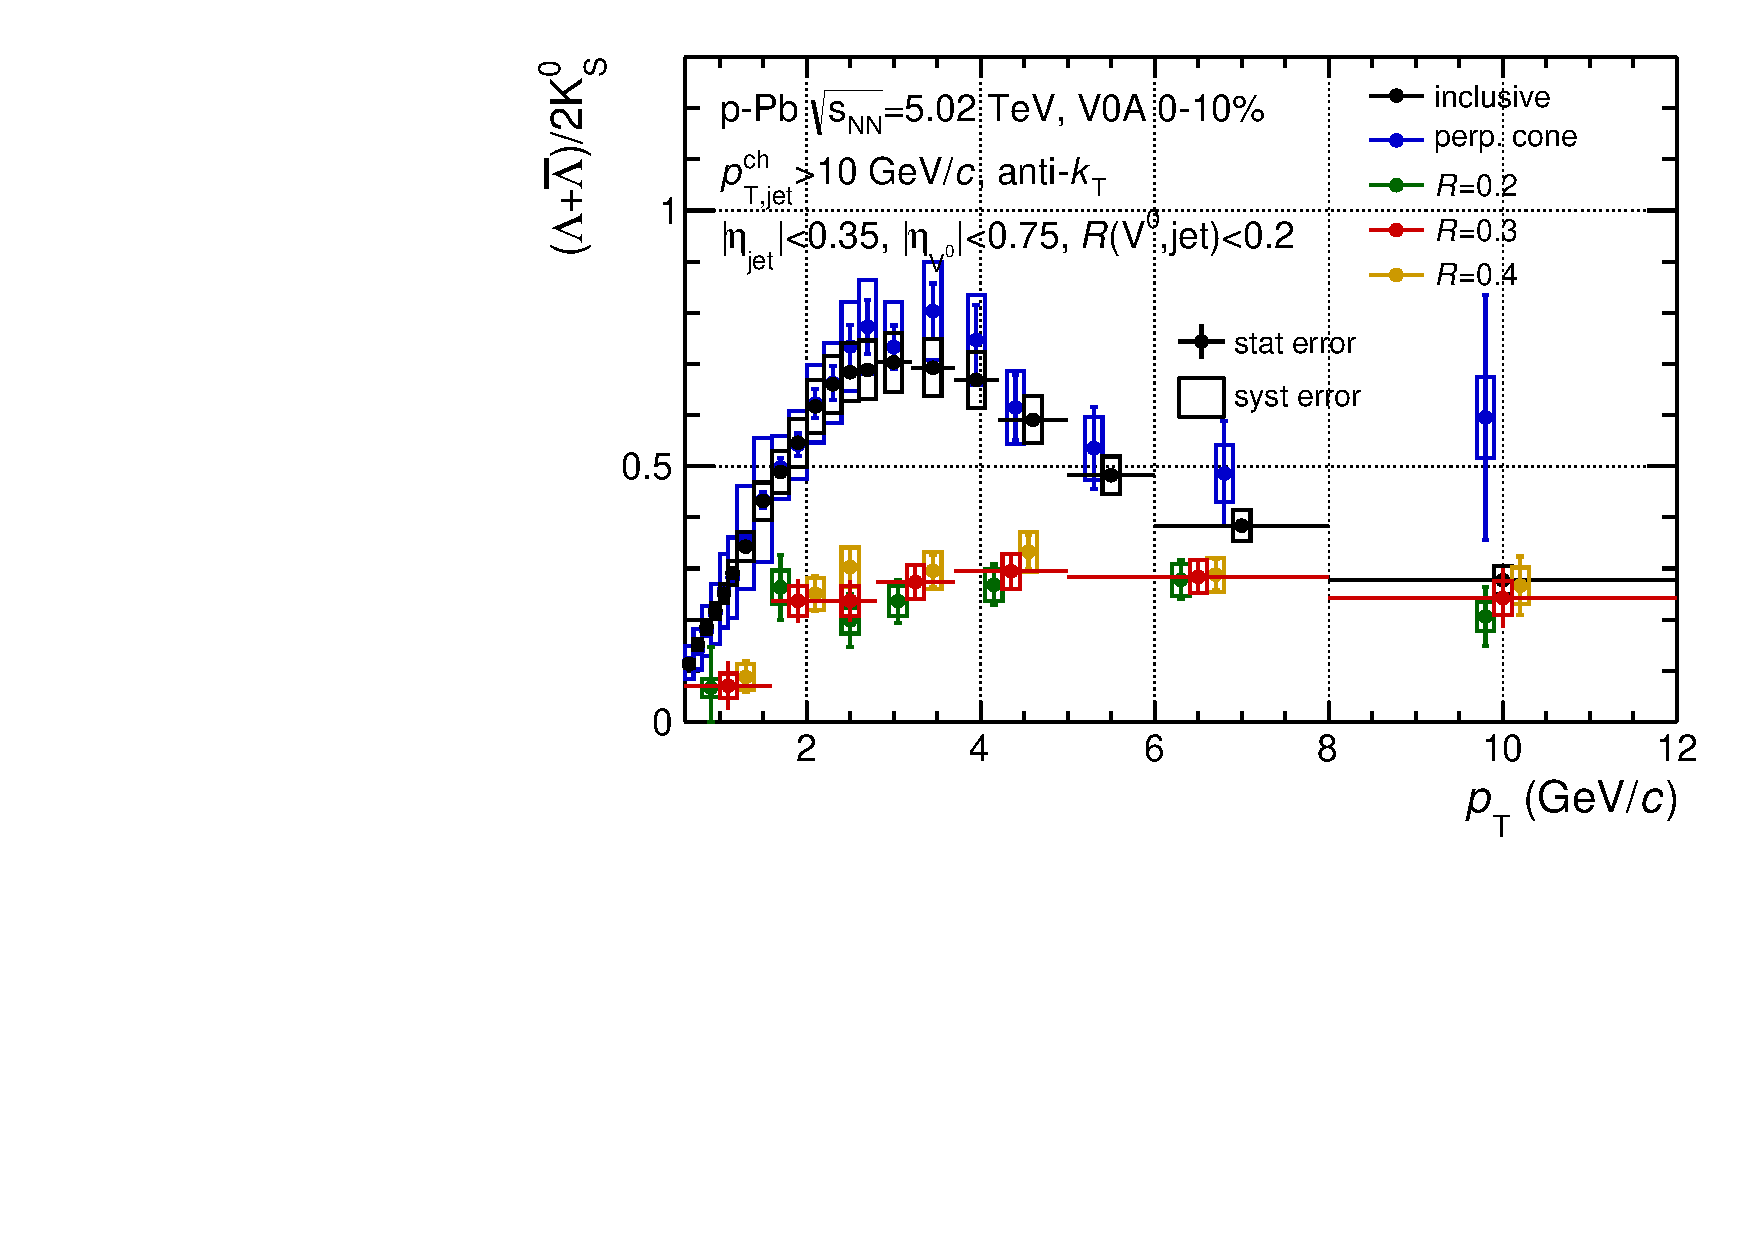
\includegraphics[width=.32\textwidth]{cL2K_Pt_Comp_JC02_V0A_000_010_PtJ10}
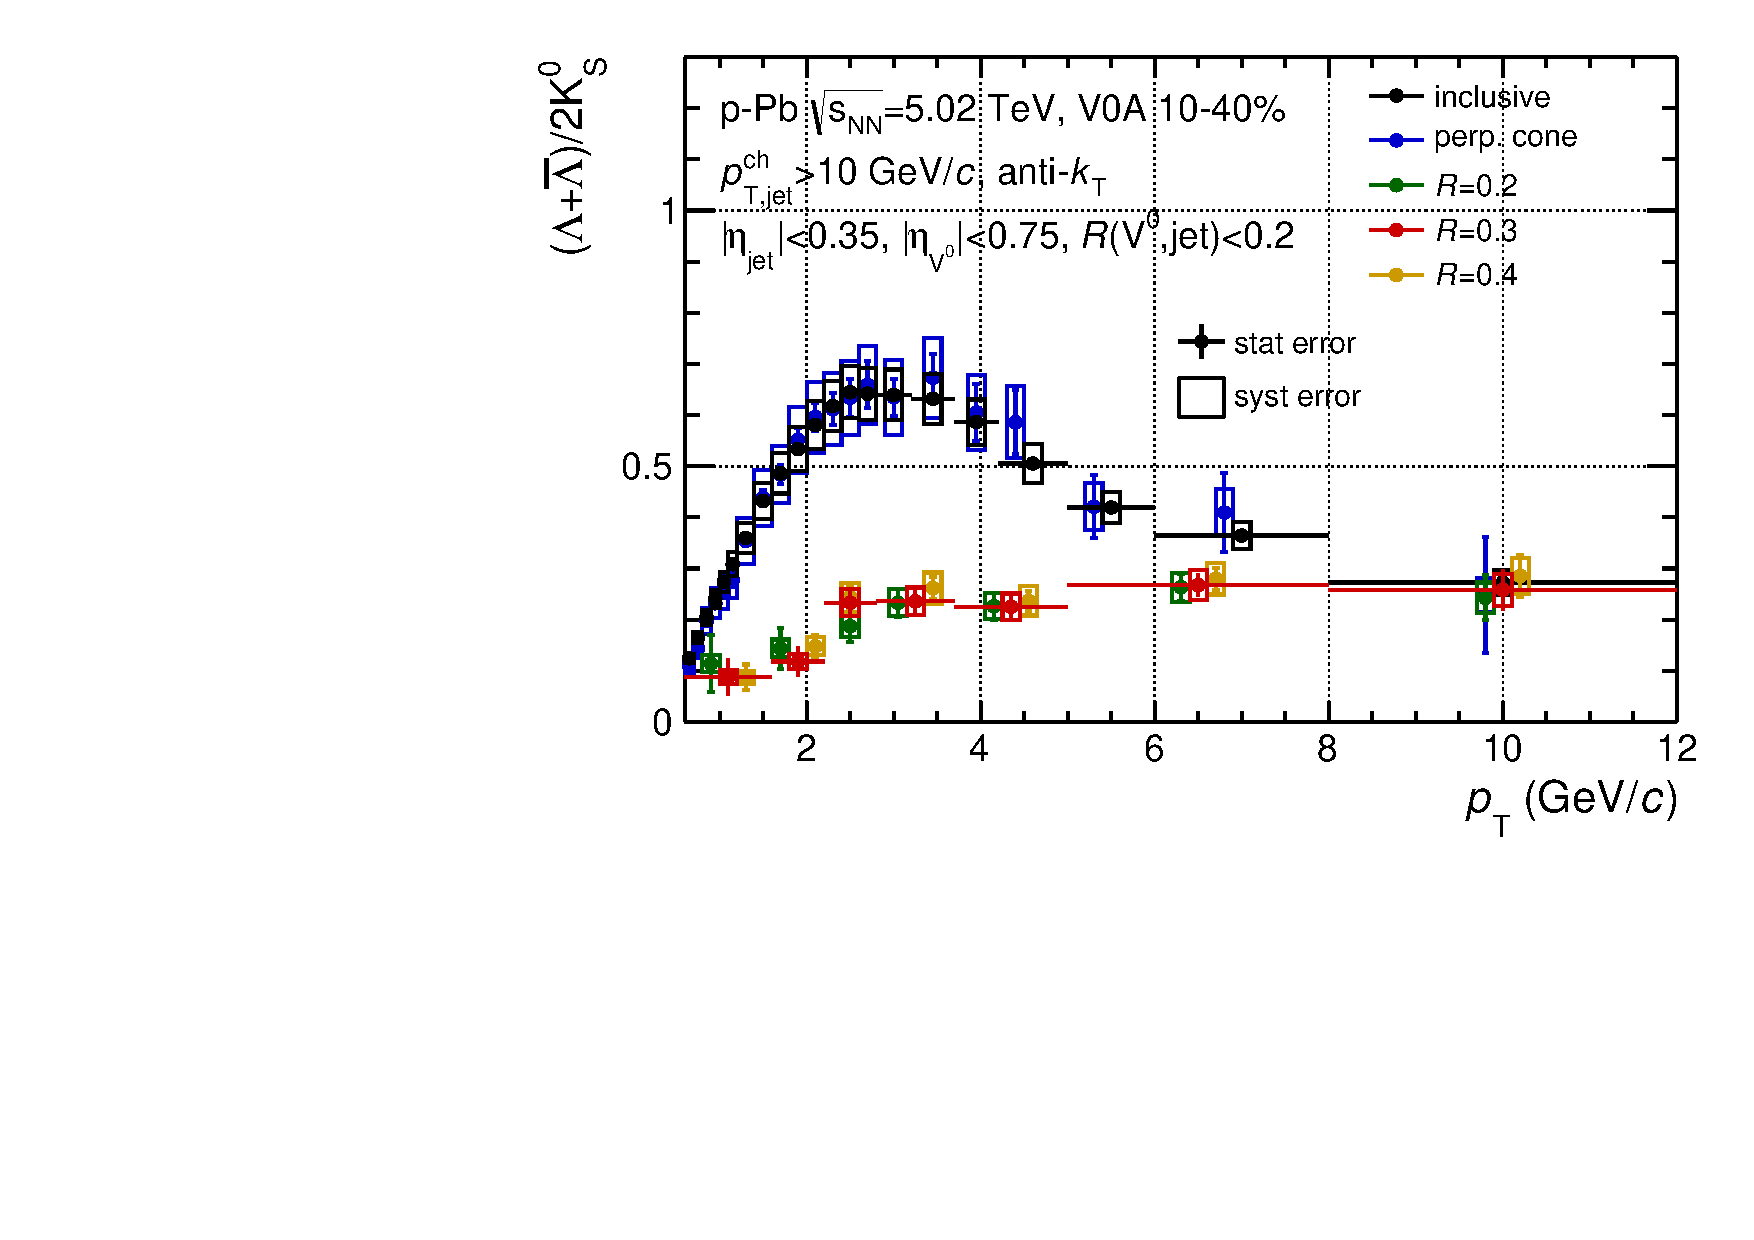
\includegraphics[width=.32\textwidth]{cL2K_Pt_Comp_JC02_V0A_010_040_PtJ10}
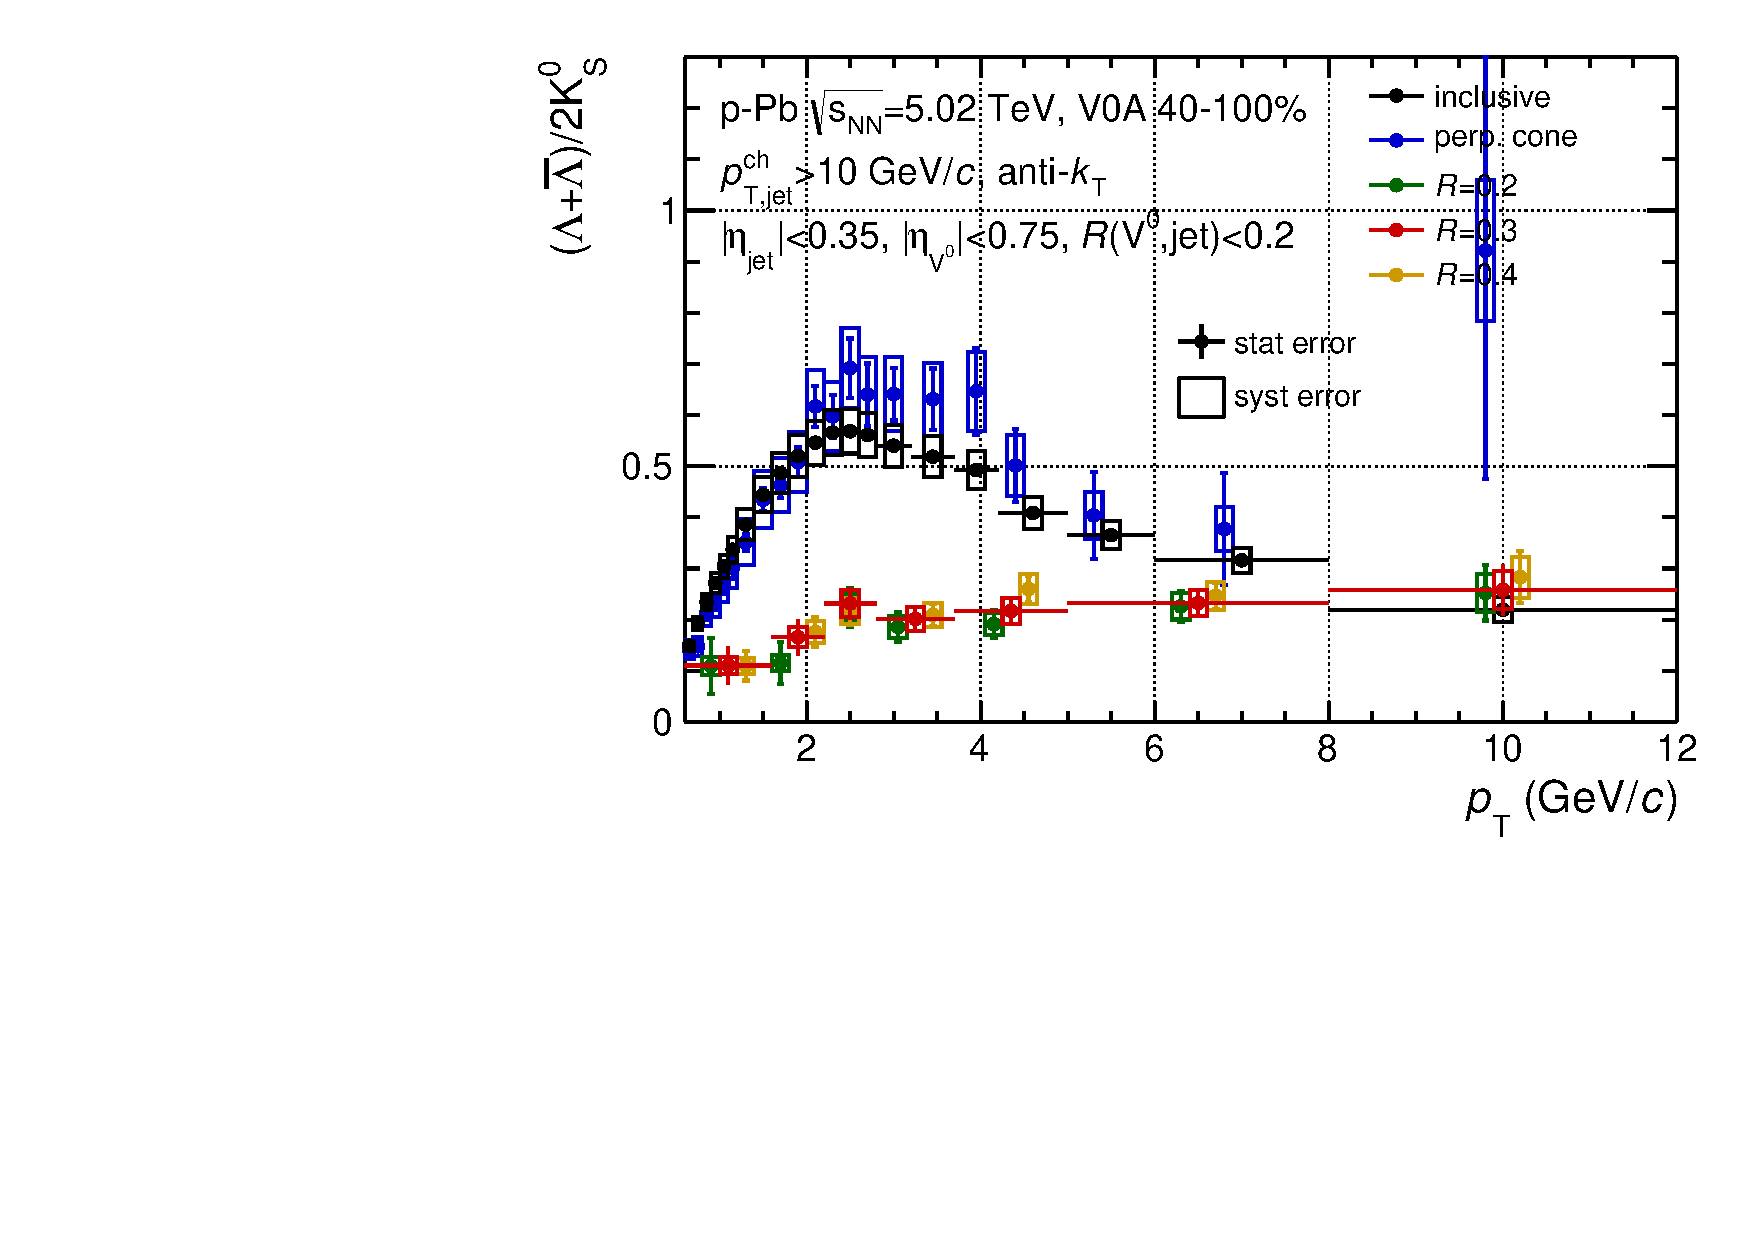
\includegraphics[width=.32\textwidth]{cL2K_Pt_Comp_JC02_V0A_040_100_PtJ10}
\caption{$\Lambda$-to-$\Kshort$ ratio as a function of $\pT$
  obtained in jets with three different jet resolution
  parameters $R=0.2,~0.3$ and $0.4$ and, $p_{\rm T,jet}>10~\GeVc$.
  The $\Vzero$--jet matching radius $R(\Vzero,{\rm jet})<0.2$.
  Results are shown in three V0A event activity classes and
  compared with the inclusive and the underlying $\Vzeros$.}
\label{fig:s01L2KJC02V0APtj10}
\end{figure}

\begin{figure}[htbp]
\centering
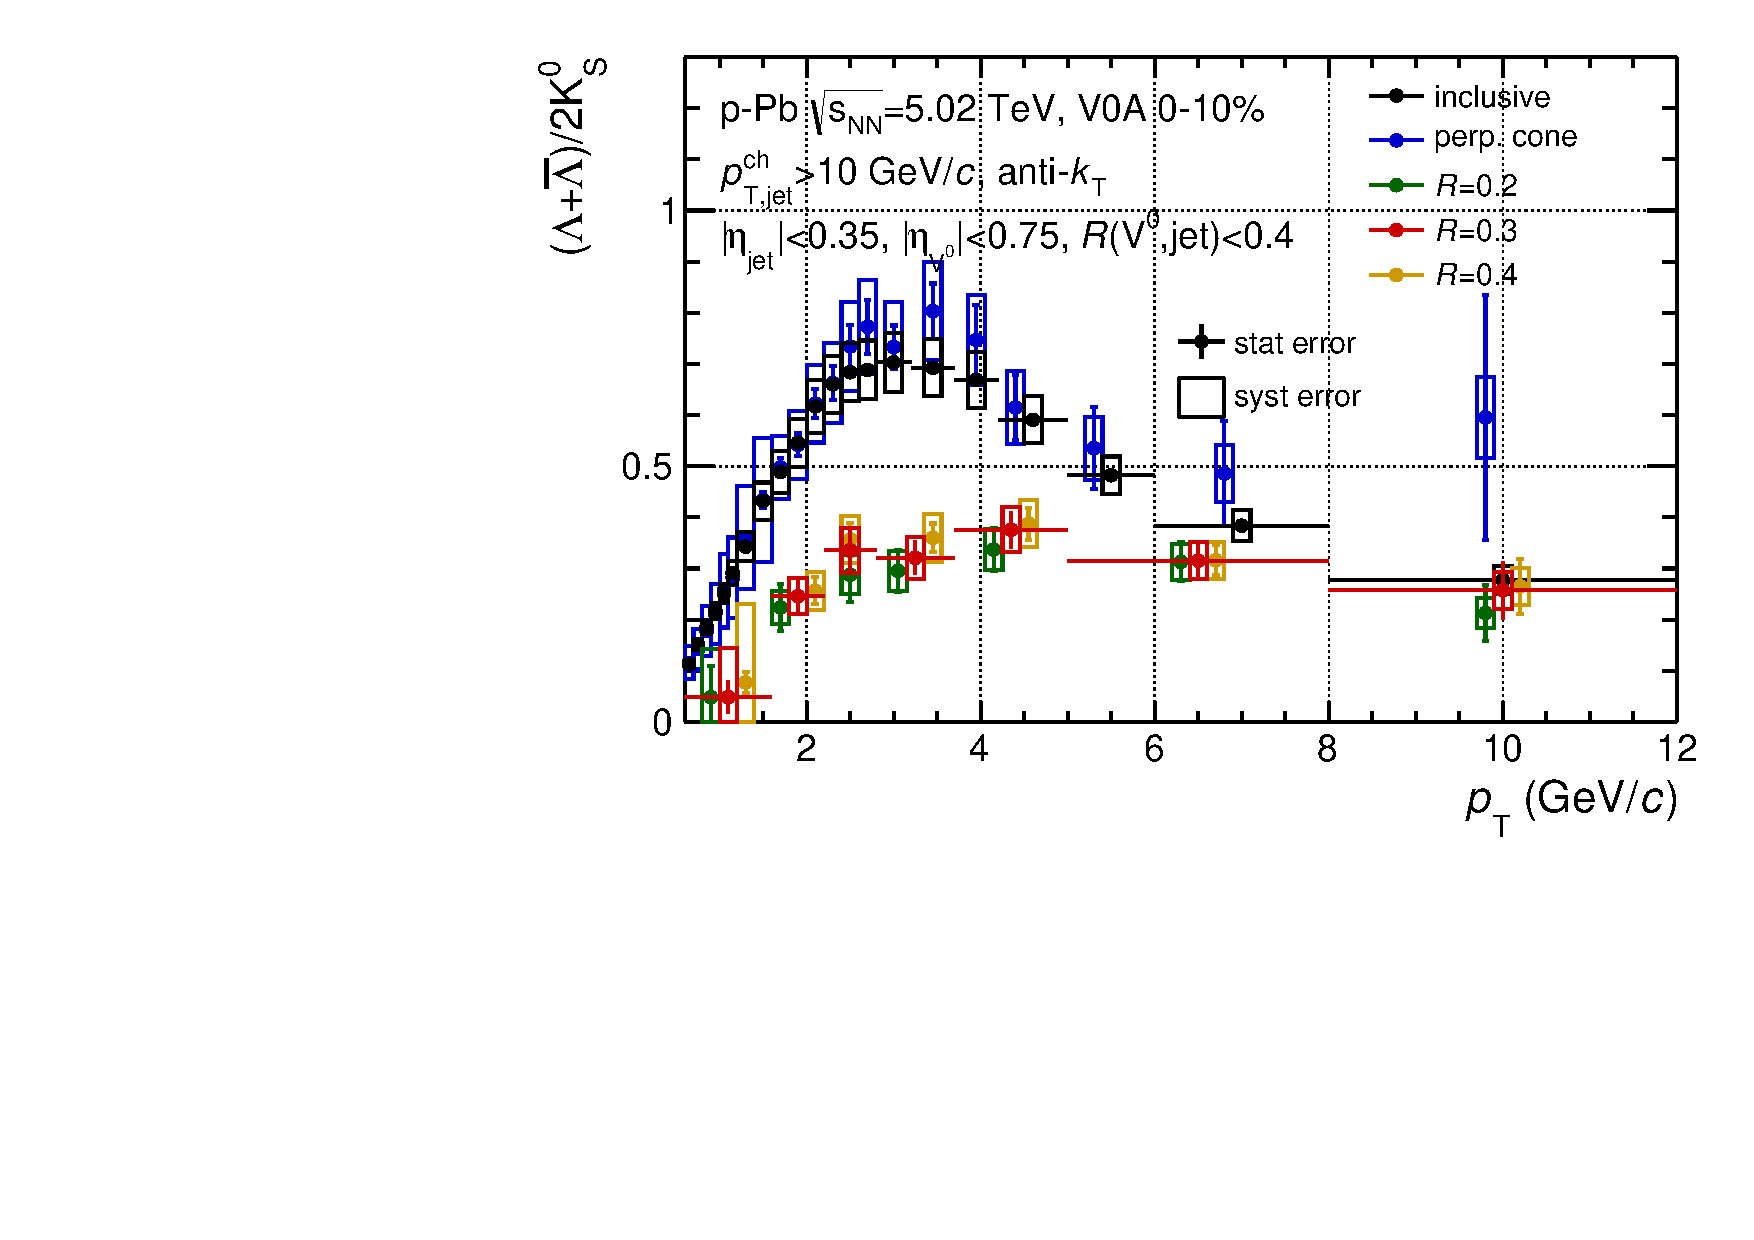
\includegraphics[width=.32\textwidth]{cL2K_Pt_Comp_JC04_V0A_000_010_PtJ10}
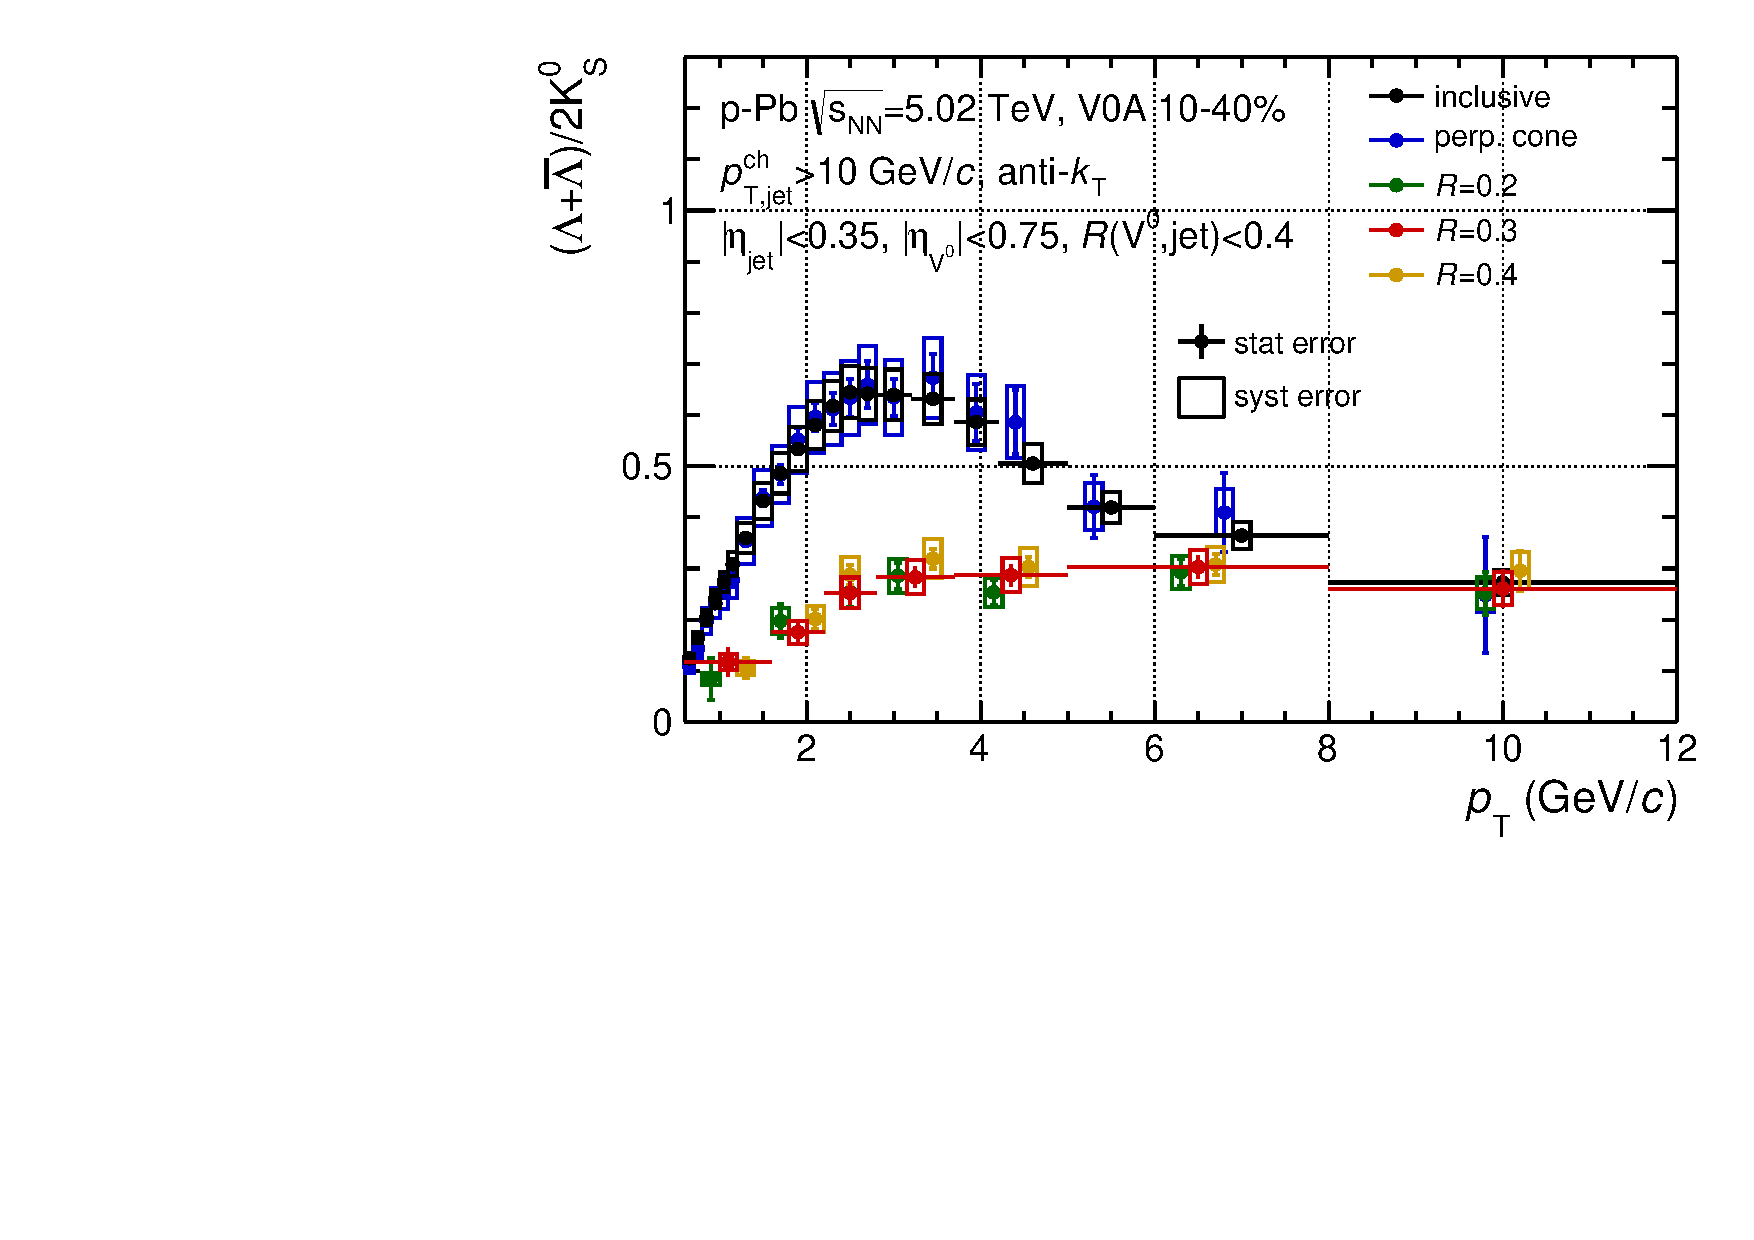
\includegraphics[width=.32\textwidth]{cL2K_Pt_Comp_JC04_V0A_010_040_PtJ10}
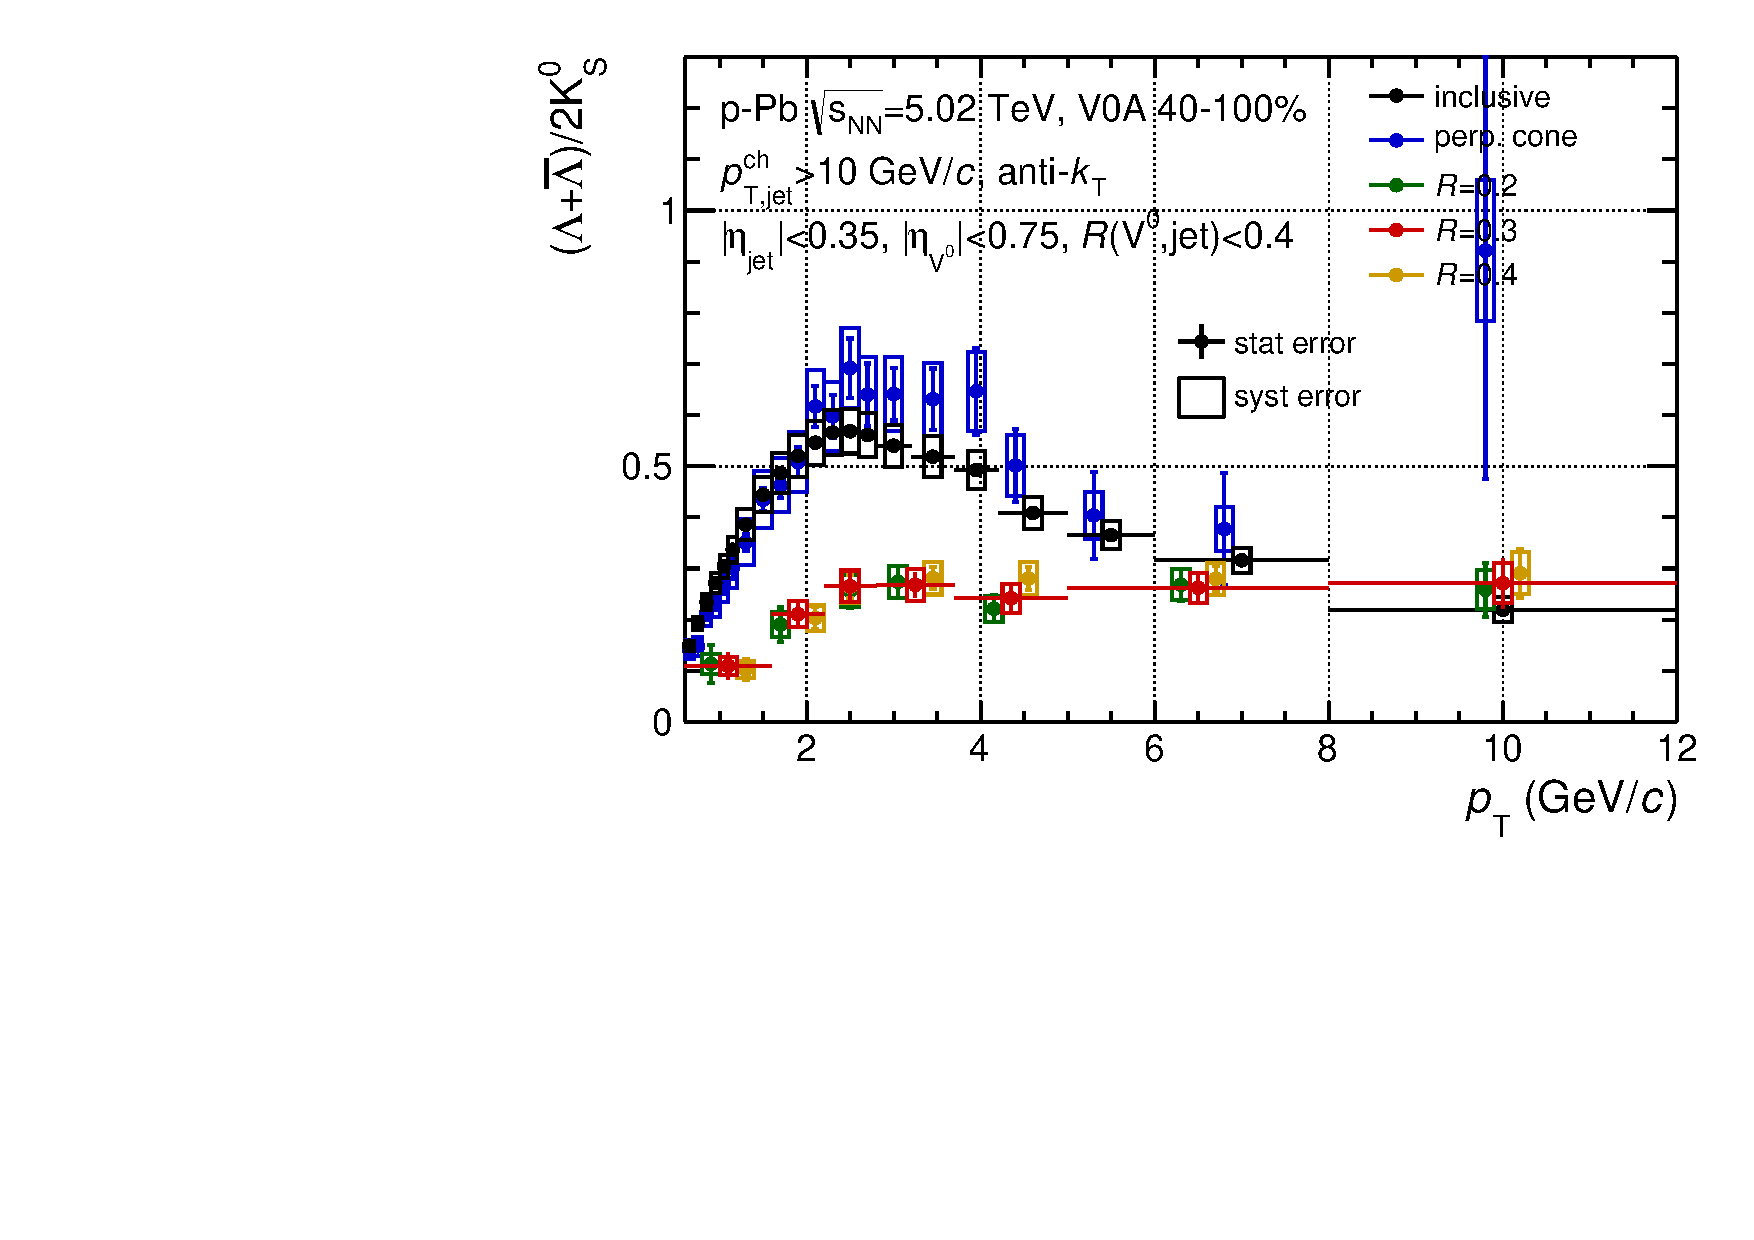
\includegraphics[width=.32\textwidth]{cL2K_Pt_Comp_JC04_V0A_040_100_PtJ10}
\caption{$\Lambda$-to-$\Kshort$ ratio as a function of $\pT$
  obtained in jets with three different jet resolution
  parameters $R=0.2,~0.3$ and $0.4$ and, $p_{\rm T,jet}>10~\GeVc$.
  The $\Vzero$--jet matching radius $R(\Vzero,{\rm jet})<0.4$.
  Results are shown in three V0A event activity classes and
  compared with the inclusive and the underlying $\Vzeros$.}
\label{fig:s01L2KJC04V0APtj10}
\end{figure}

\begin{figure}[htbp]
\centering
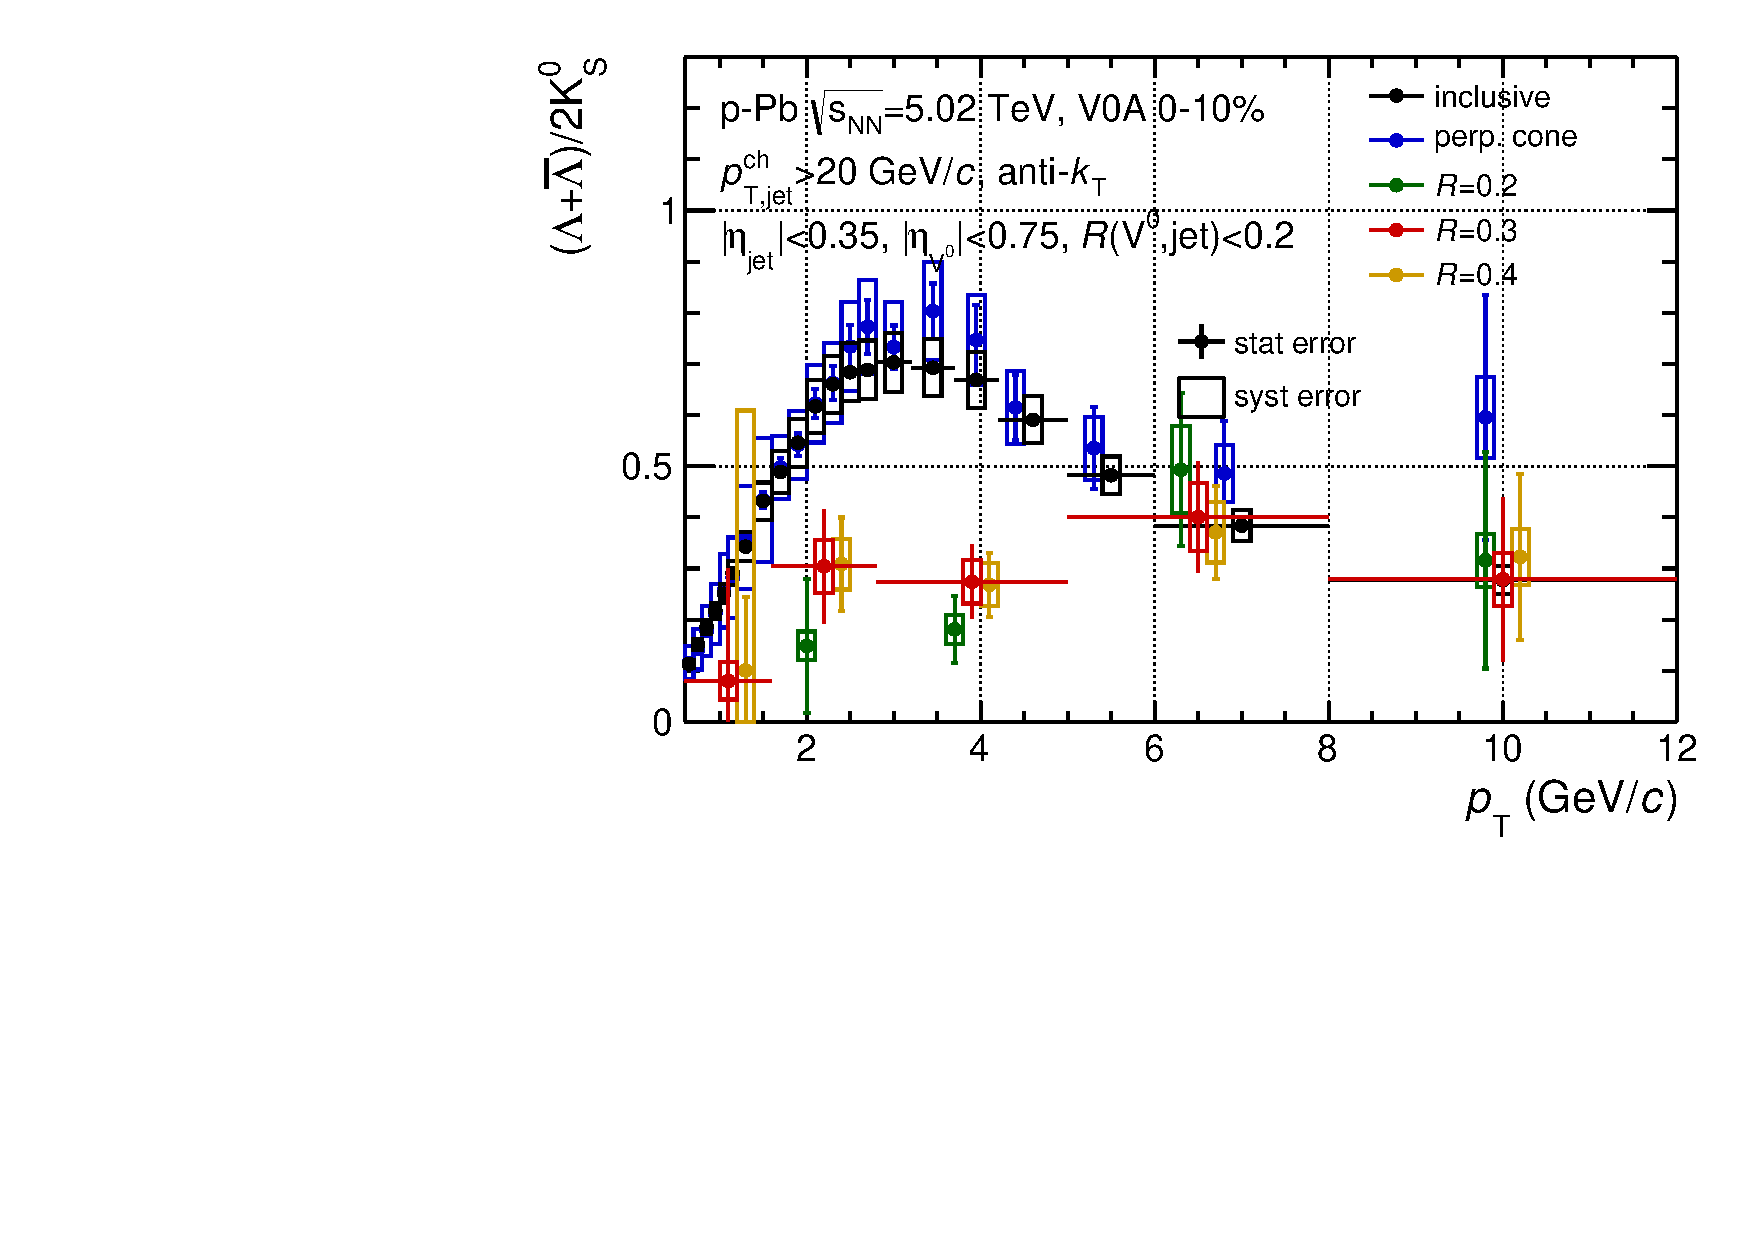
\includegraphics[width=.32\textwidth]{cL2K_Pt_Comp_JC02_V0A_000_010_PtJ20}
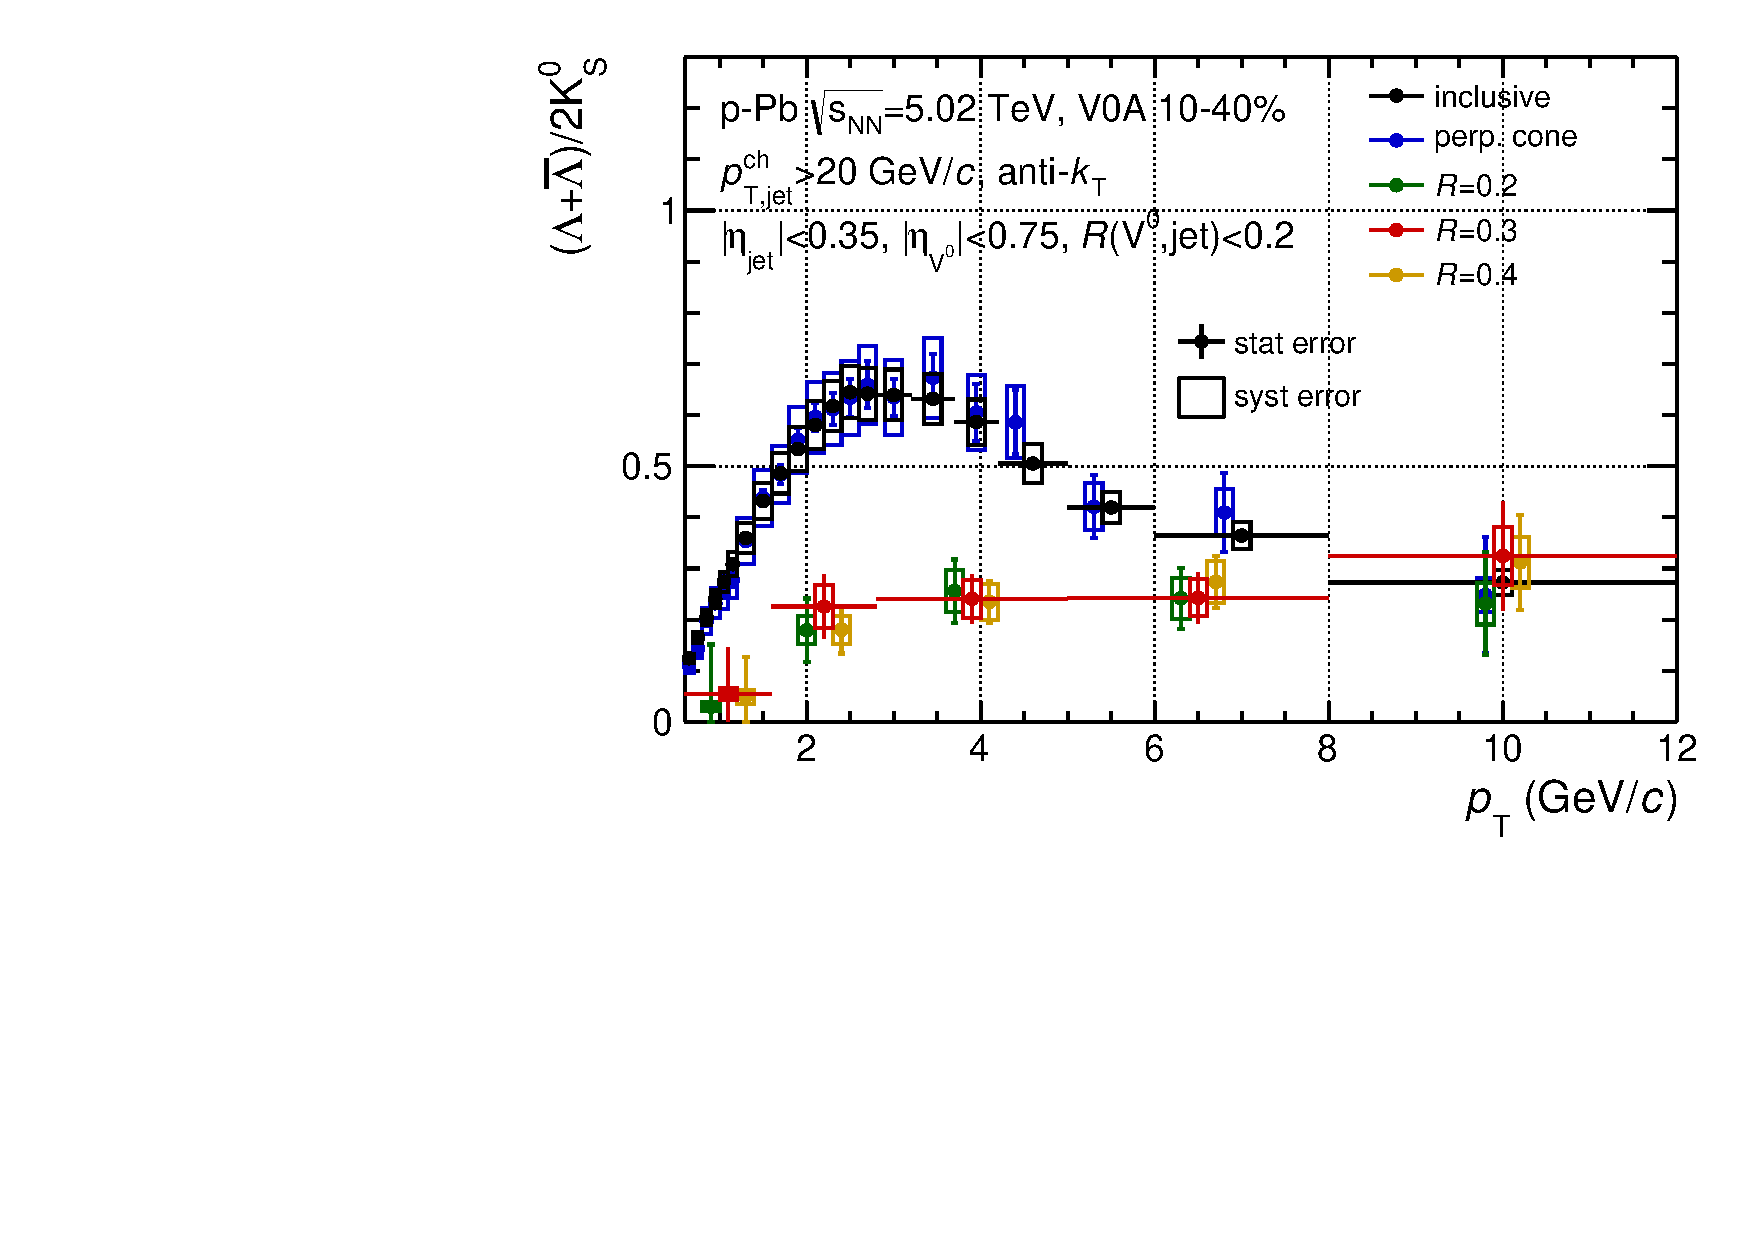
\includegraphics[width=.32\textwidth]{cL2K_Pt_Comp_JC02_V0A_010_040_PtJ20}
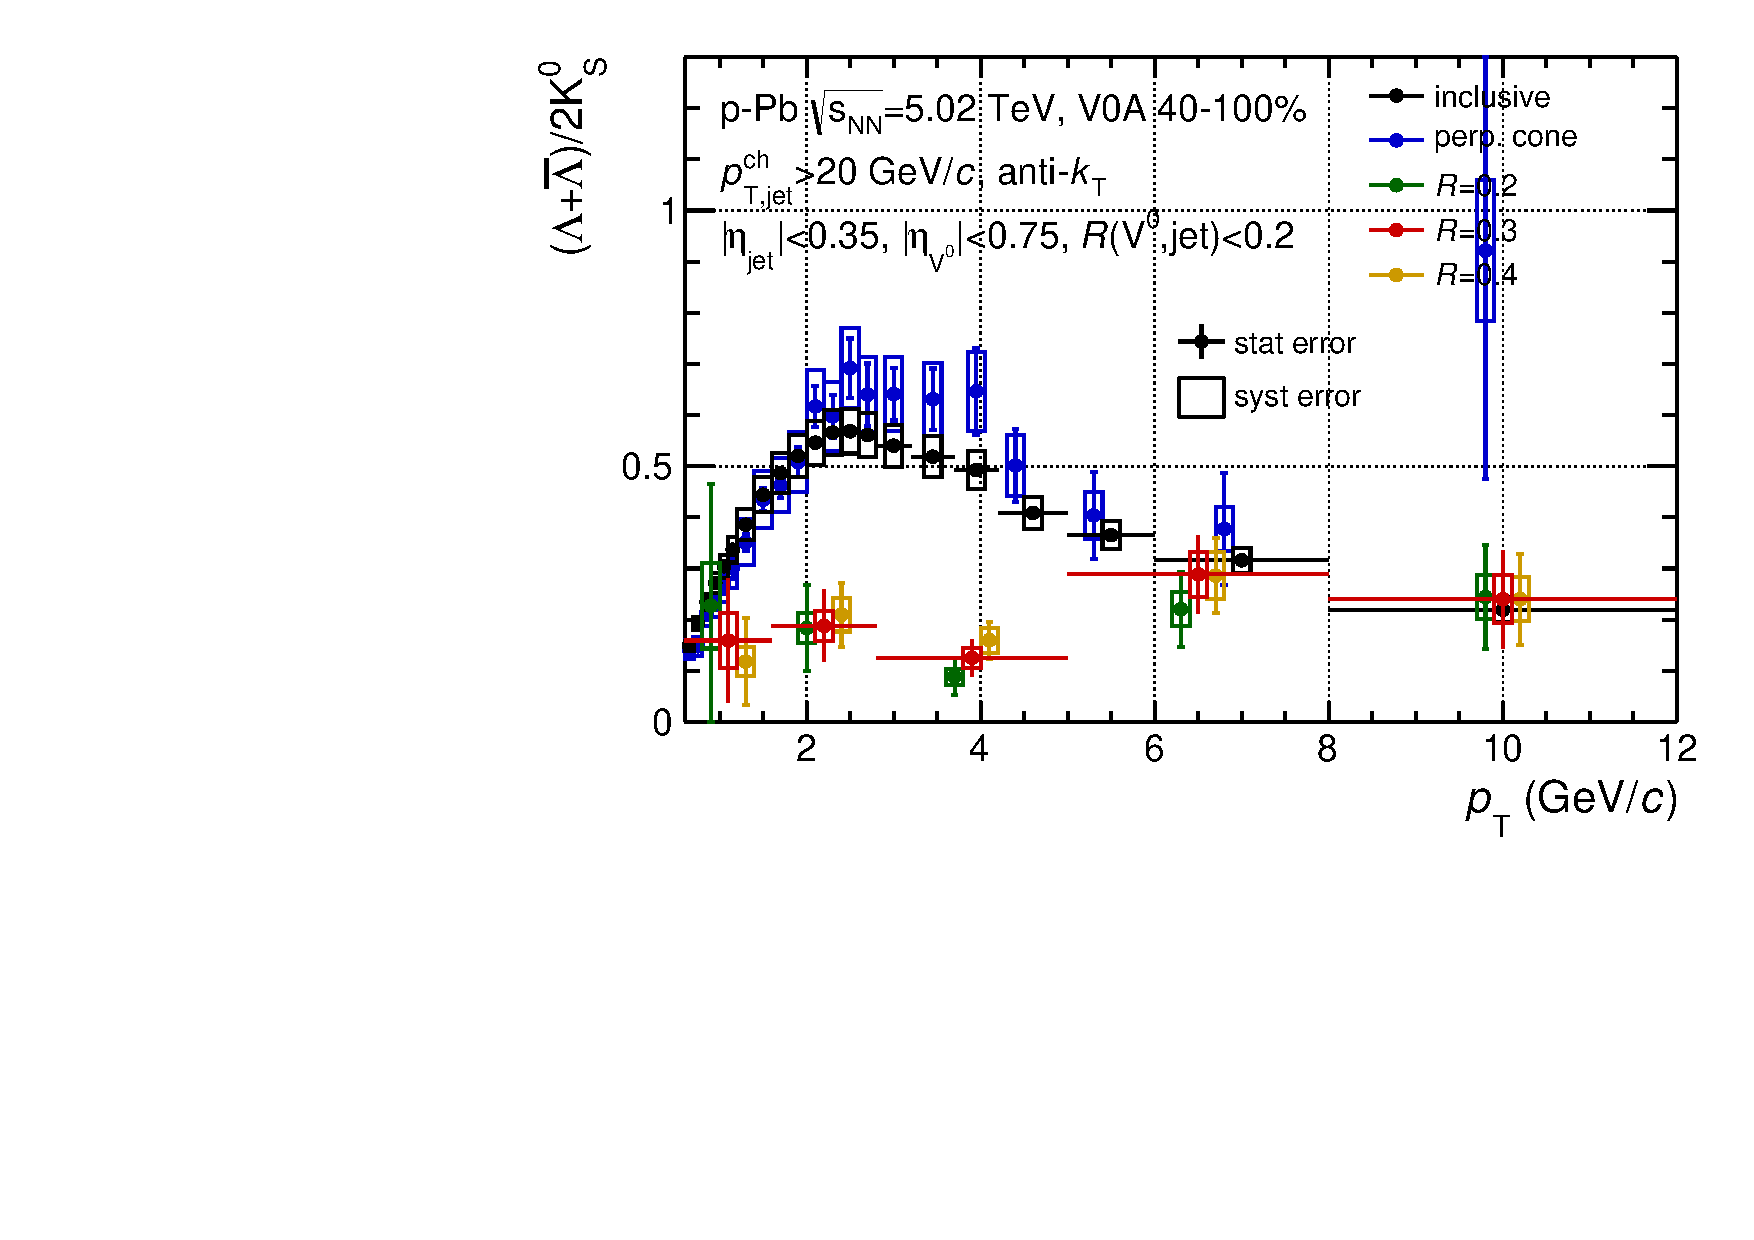
\includegraphics[width=.32\textwidth]{cL2K_Pt_Comp_JC02_V0A_040_100_PtJ20}
\caption{$\Lambda$-to-$\Kshort$ ratio as a function of $\pT$
  obtained in jets with three different jet resolution
  parameters $R=0.2,~0.3$ and $0.4$ and, $p_{\rm T,jet}>20~\GeVc$.
  The $\Vzero$--jet matching radius $R(\Vzero,{\rm jet})<0.2$.
  Results are shown in three V0A event activity classes and
  compared with the inclusive and the underlying $\Vzeros$.}
\label{fig:s01L2KJC02V0APtj20}
\end{figure}

\begin{figure}[htbp]
\centering
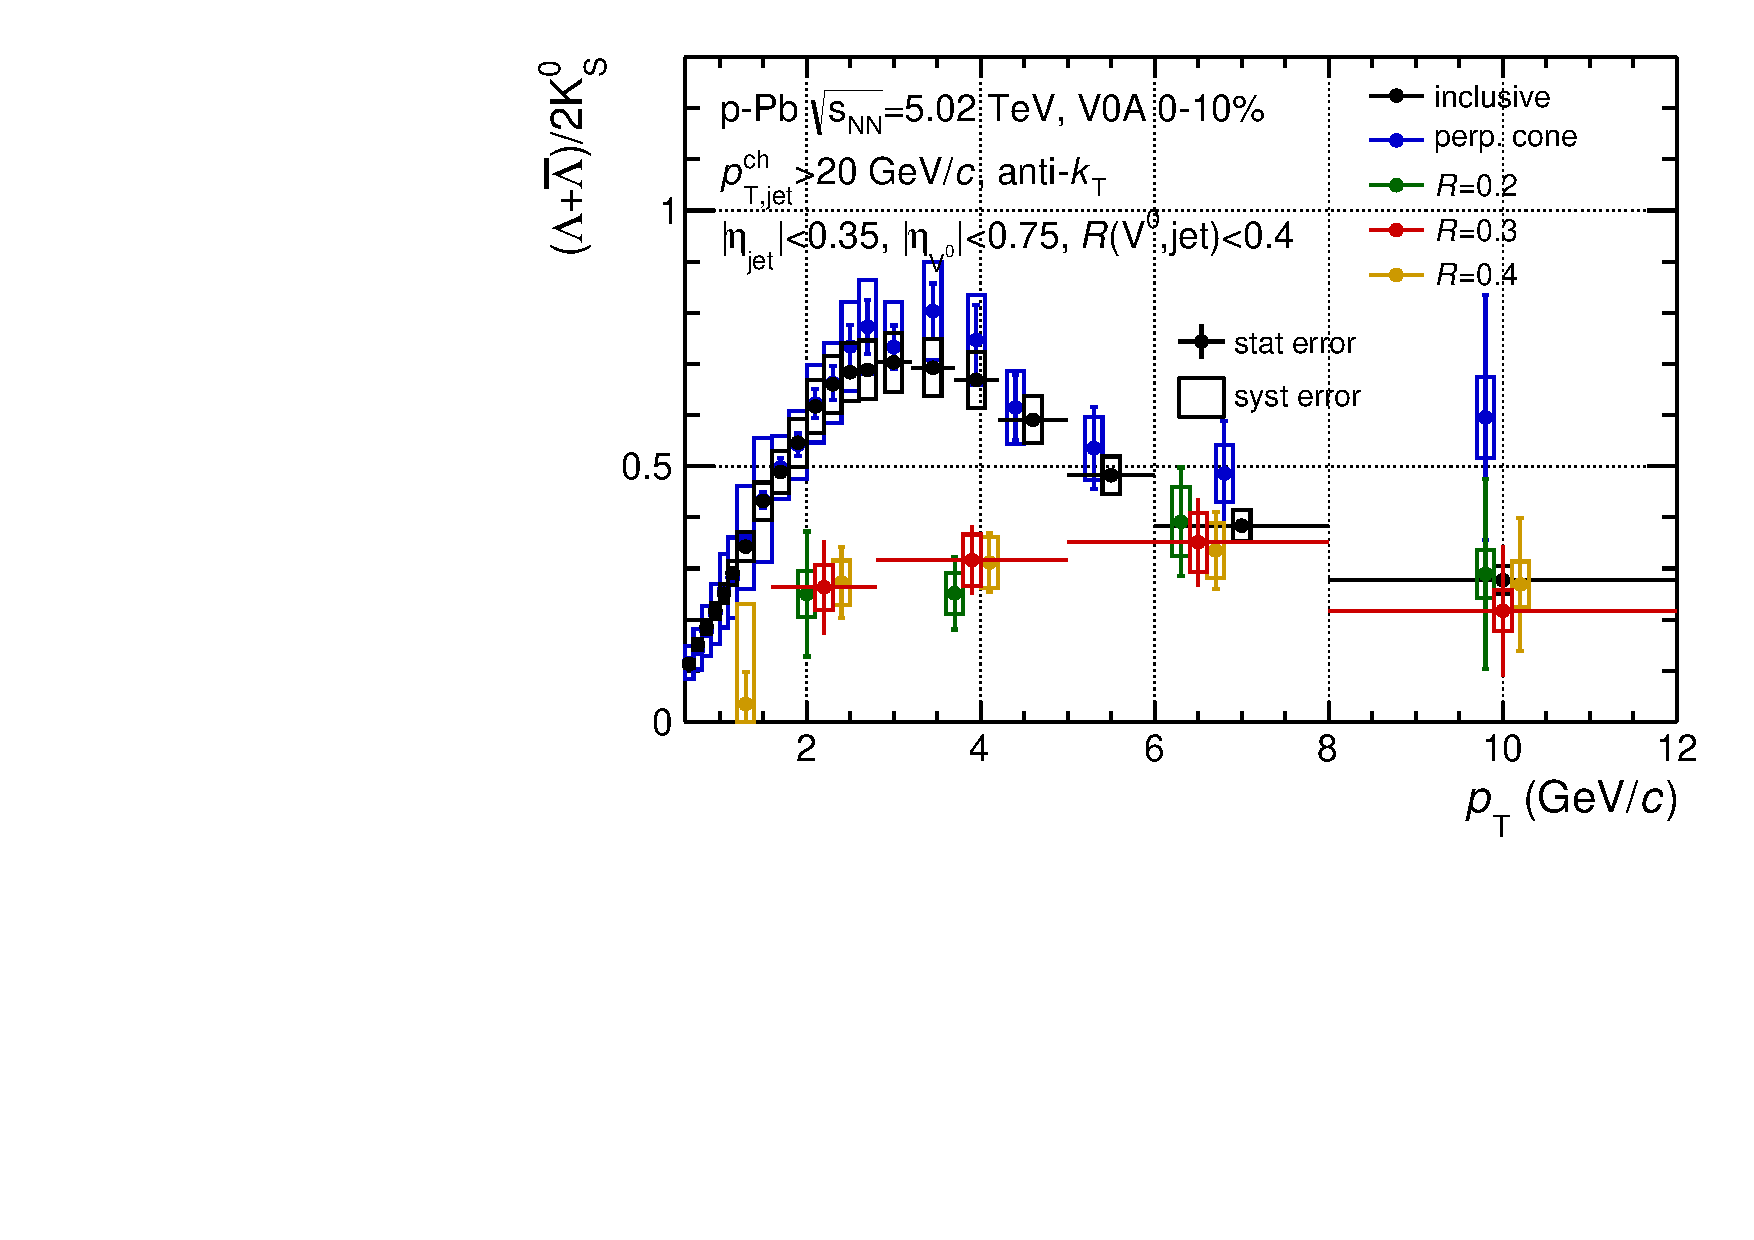
\includegraphics[width=.32\textwidth]{cL2K_Pt_Comp_JC04_V0A_000_010_PtJ20}
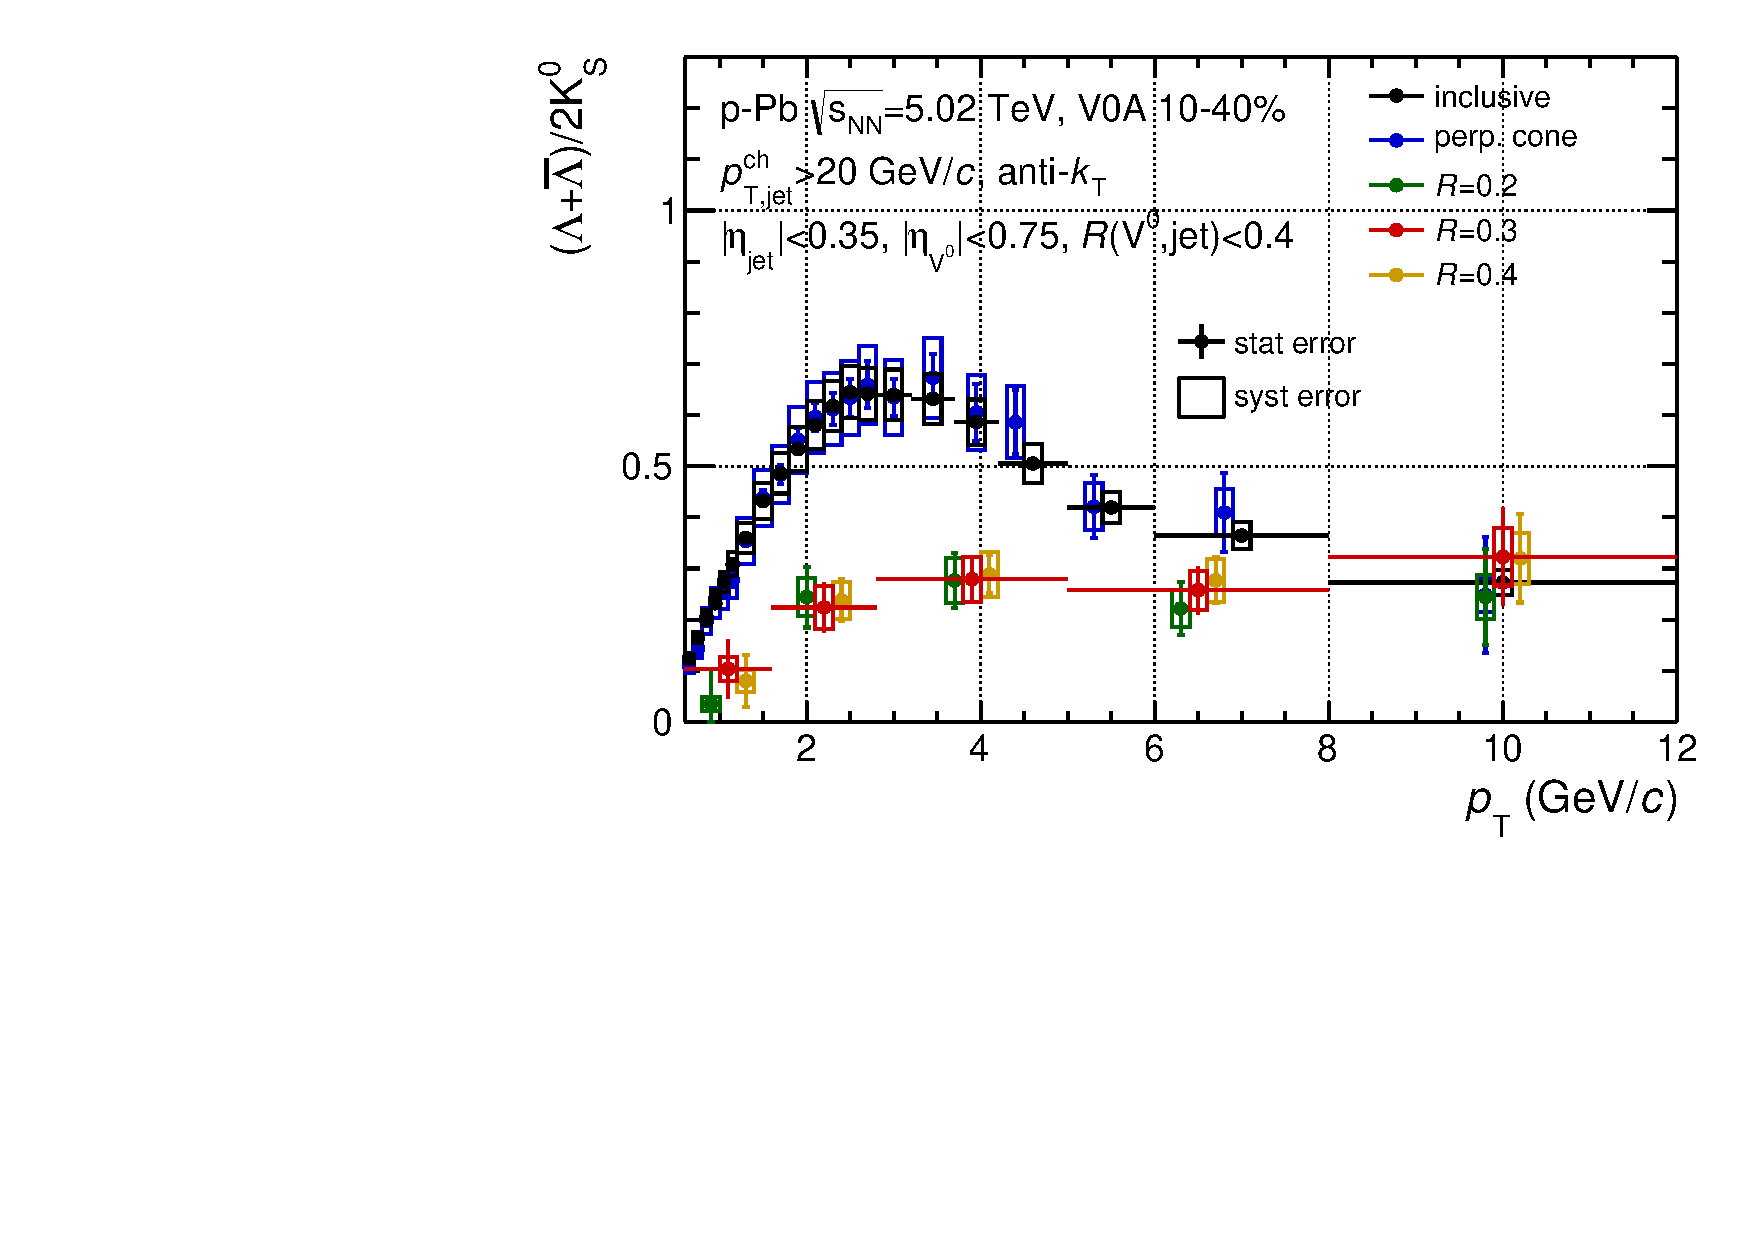
\includegraphics[width=.32\textwidth]{cL2K_Pt_Comp_JC04_V0A_010_040_PtJ20}
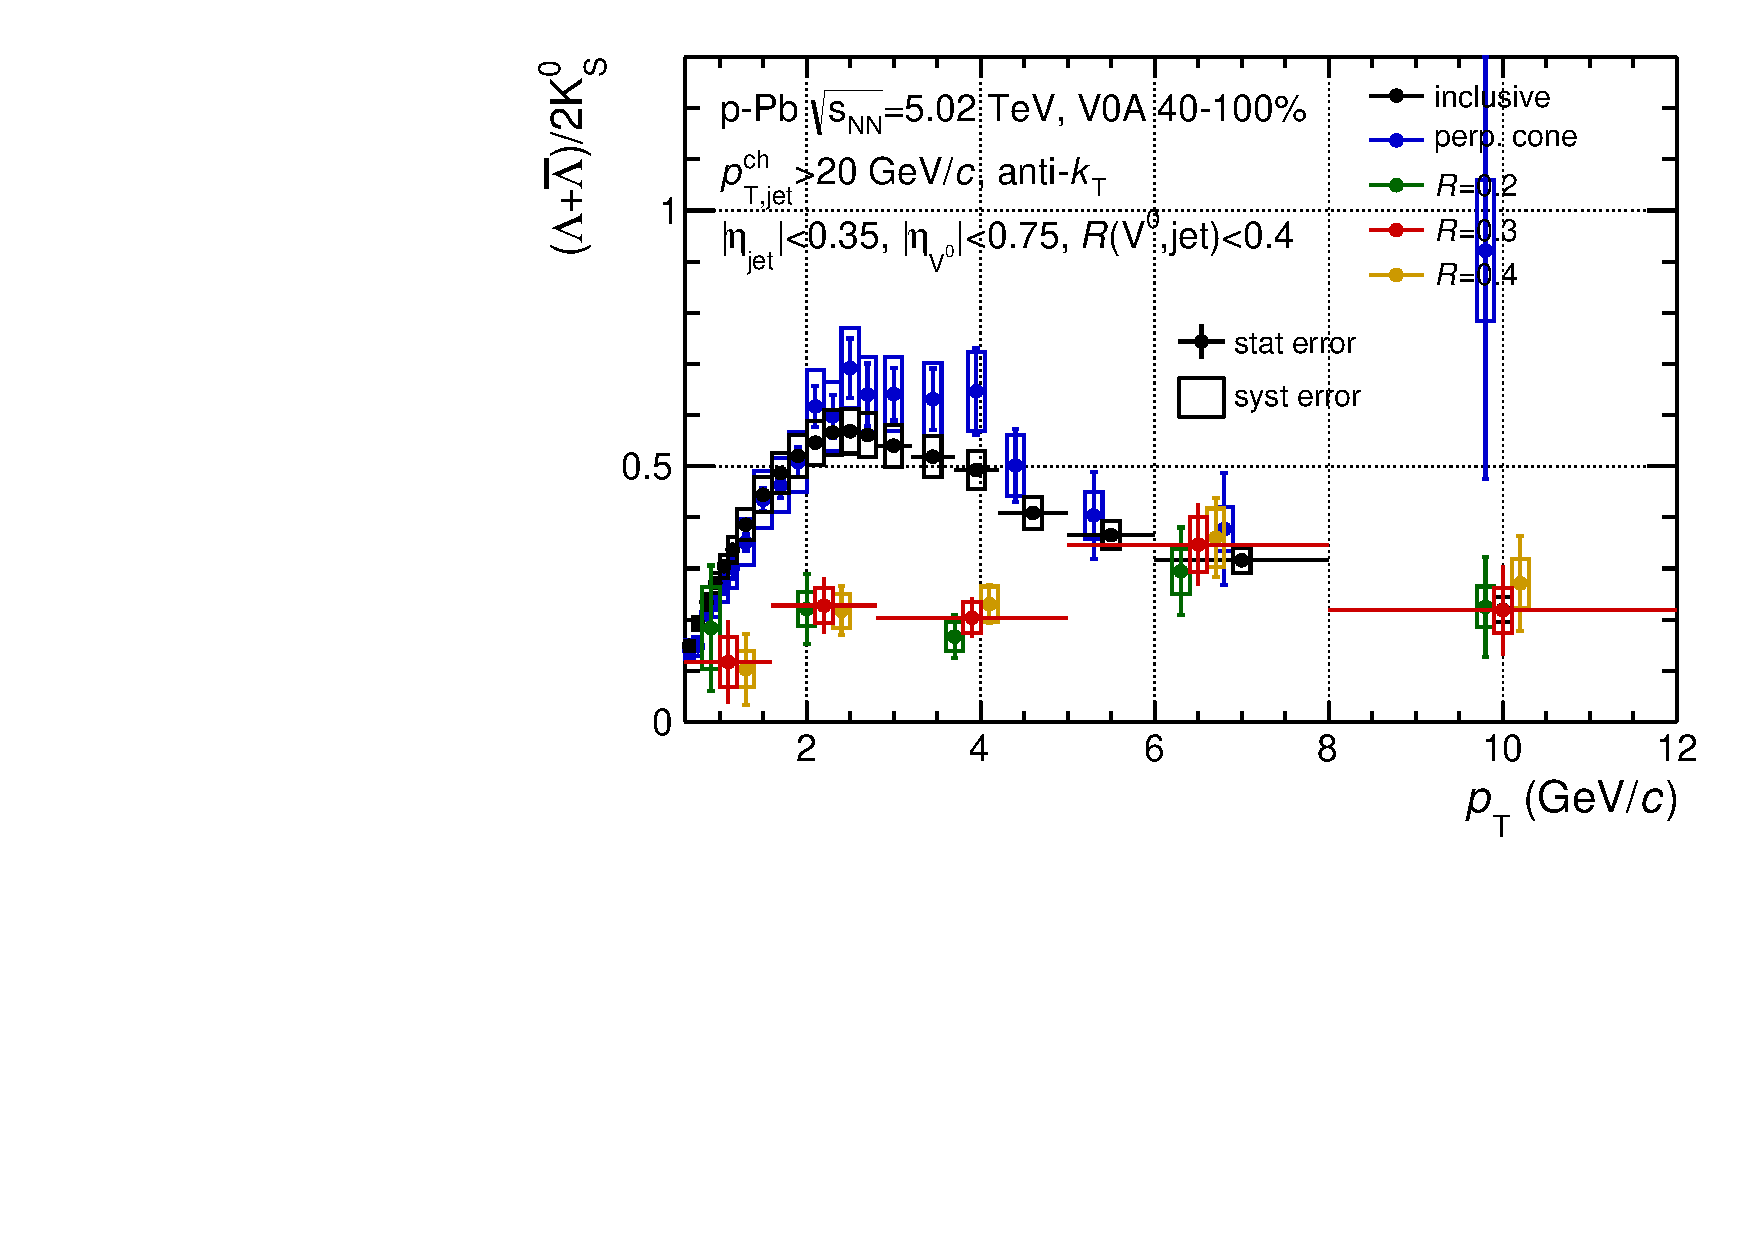
\includegraphics[width=.32\textwidth]{cL2K_Pt_Comp_JC04_V0A_040_100_PtJ20}
\caption{$\Lambda$-to-$\Kshort$ ratio as a function of $\pT$
  obtained in jets with three different jet resolution
  parameters $R=0.2,~0.3$ and $0.4$ and, $p_{\rm T,jet}>20~\GeVc$.
  The $\Vzero$--jet matching radius $R(\Vzero,{\rm jet})<0.4$.
  Results are shown in three V0A event activity classes and
  compared with the inclusive and the underlying $\Vzeros$.}
\label{fig:s01L2KJC04V0APtj20}
\end{figure}
%%%%%%%%%%%%%%%%%%%%%%%%%%%%%%%%%%%%%%%%%%%%%%%%%%%%%%%%%%%%%%%%%%%%%%%%%%%%%%%

\newpage
\subsubsection{ZNA Event Activity Estimator}

\begin{figure}[htbp]
\centering
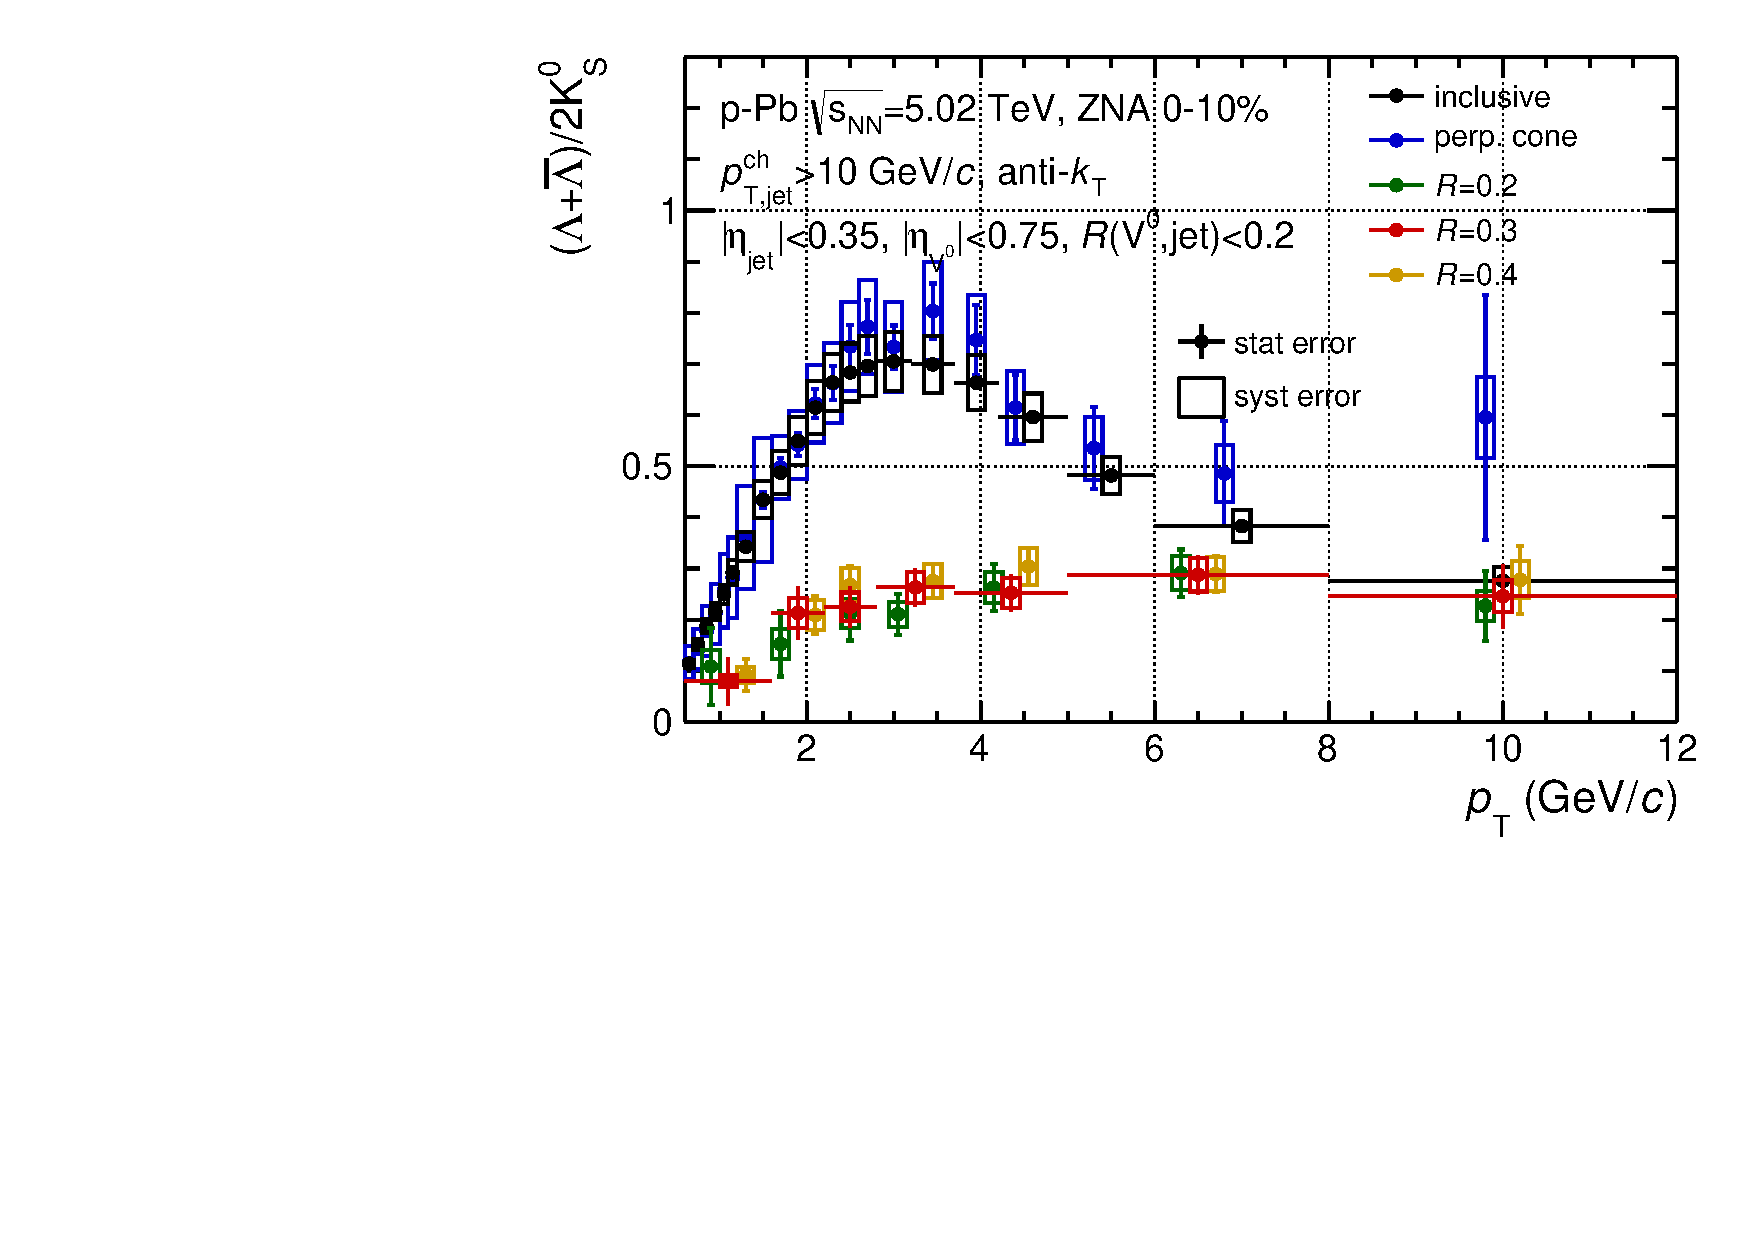
\includegraphics[width=.32\textwidth]{cL2K_Pt_Comp_JC02_ZNA_000_010_PtJ10}
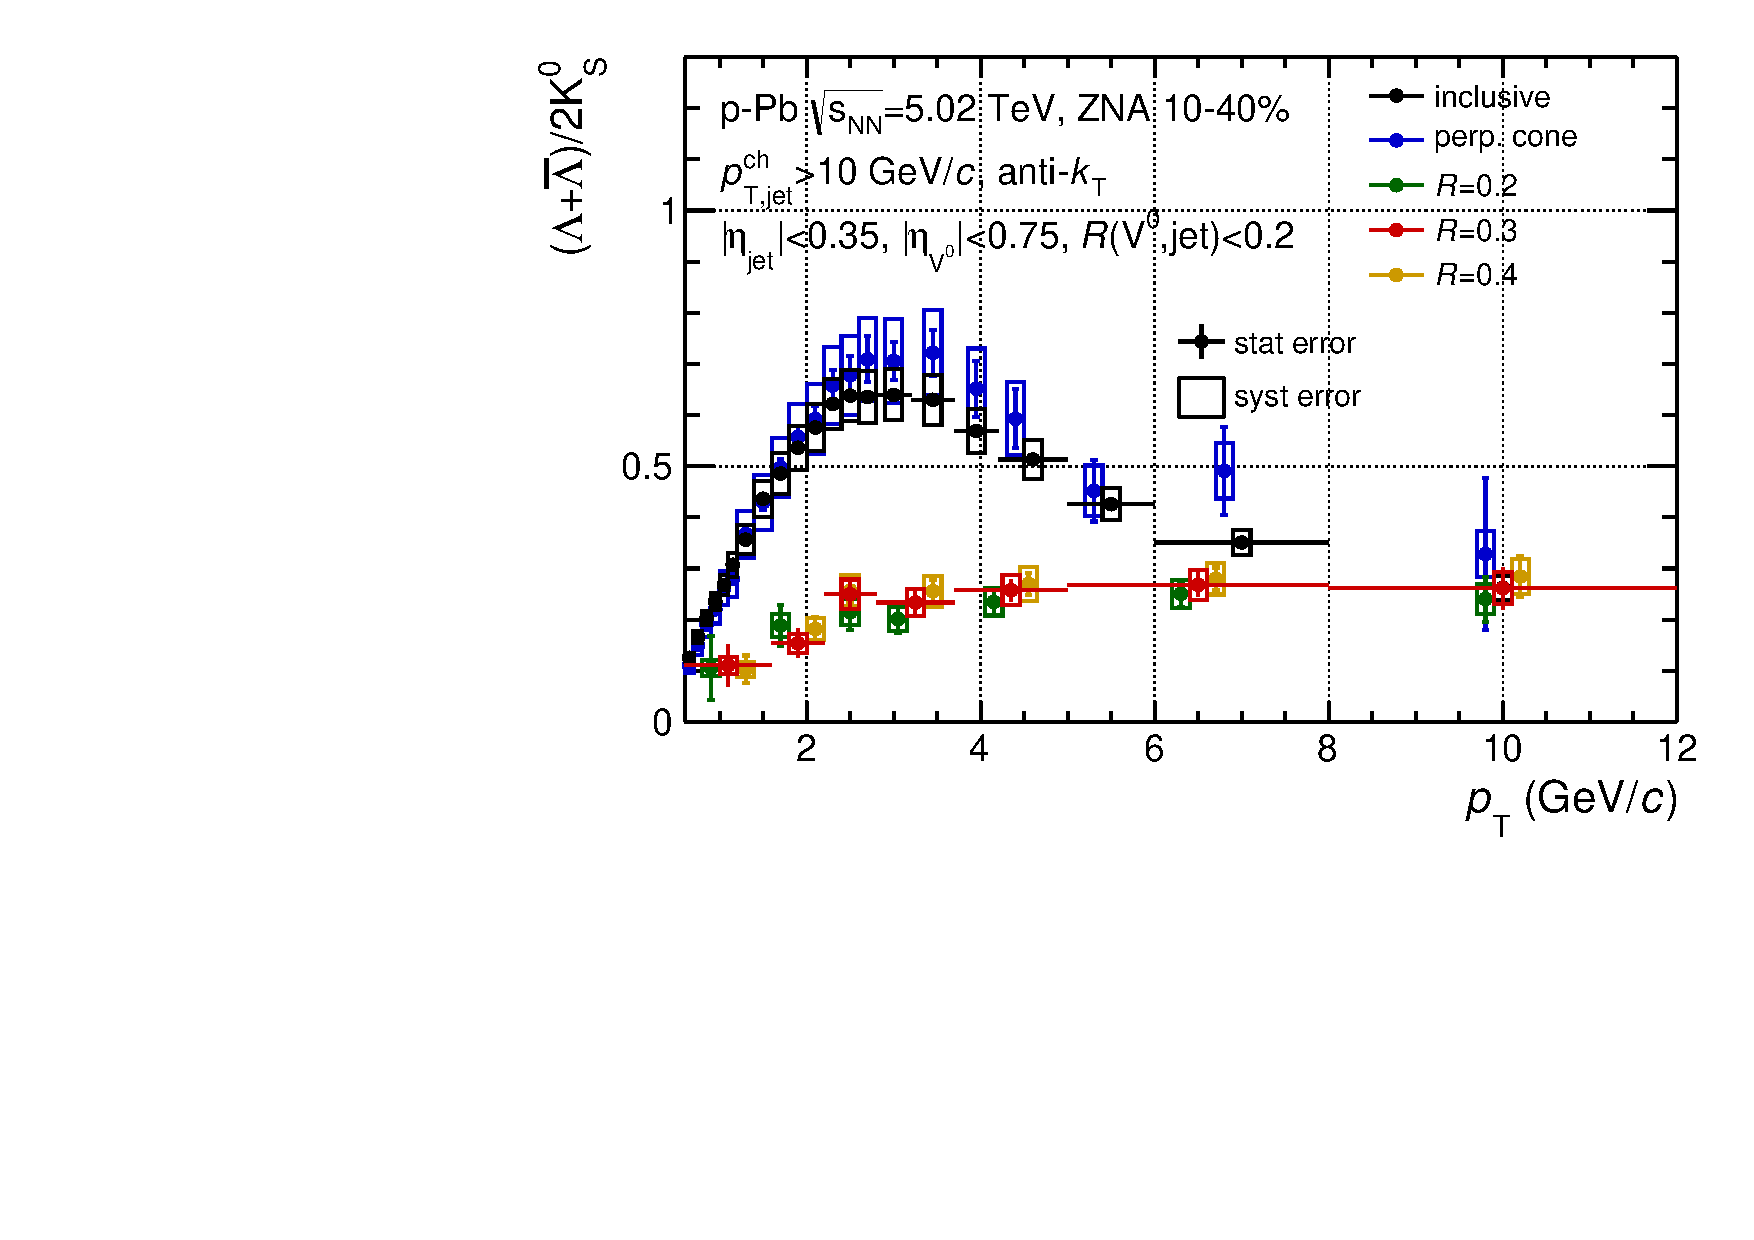
\includegraphics[width=.32\textwidth]{cL2K_Pt_Comp_JC02_ZNA_010_040_PtJ10}
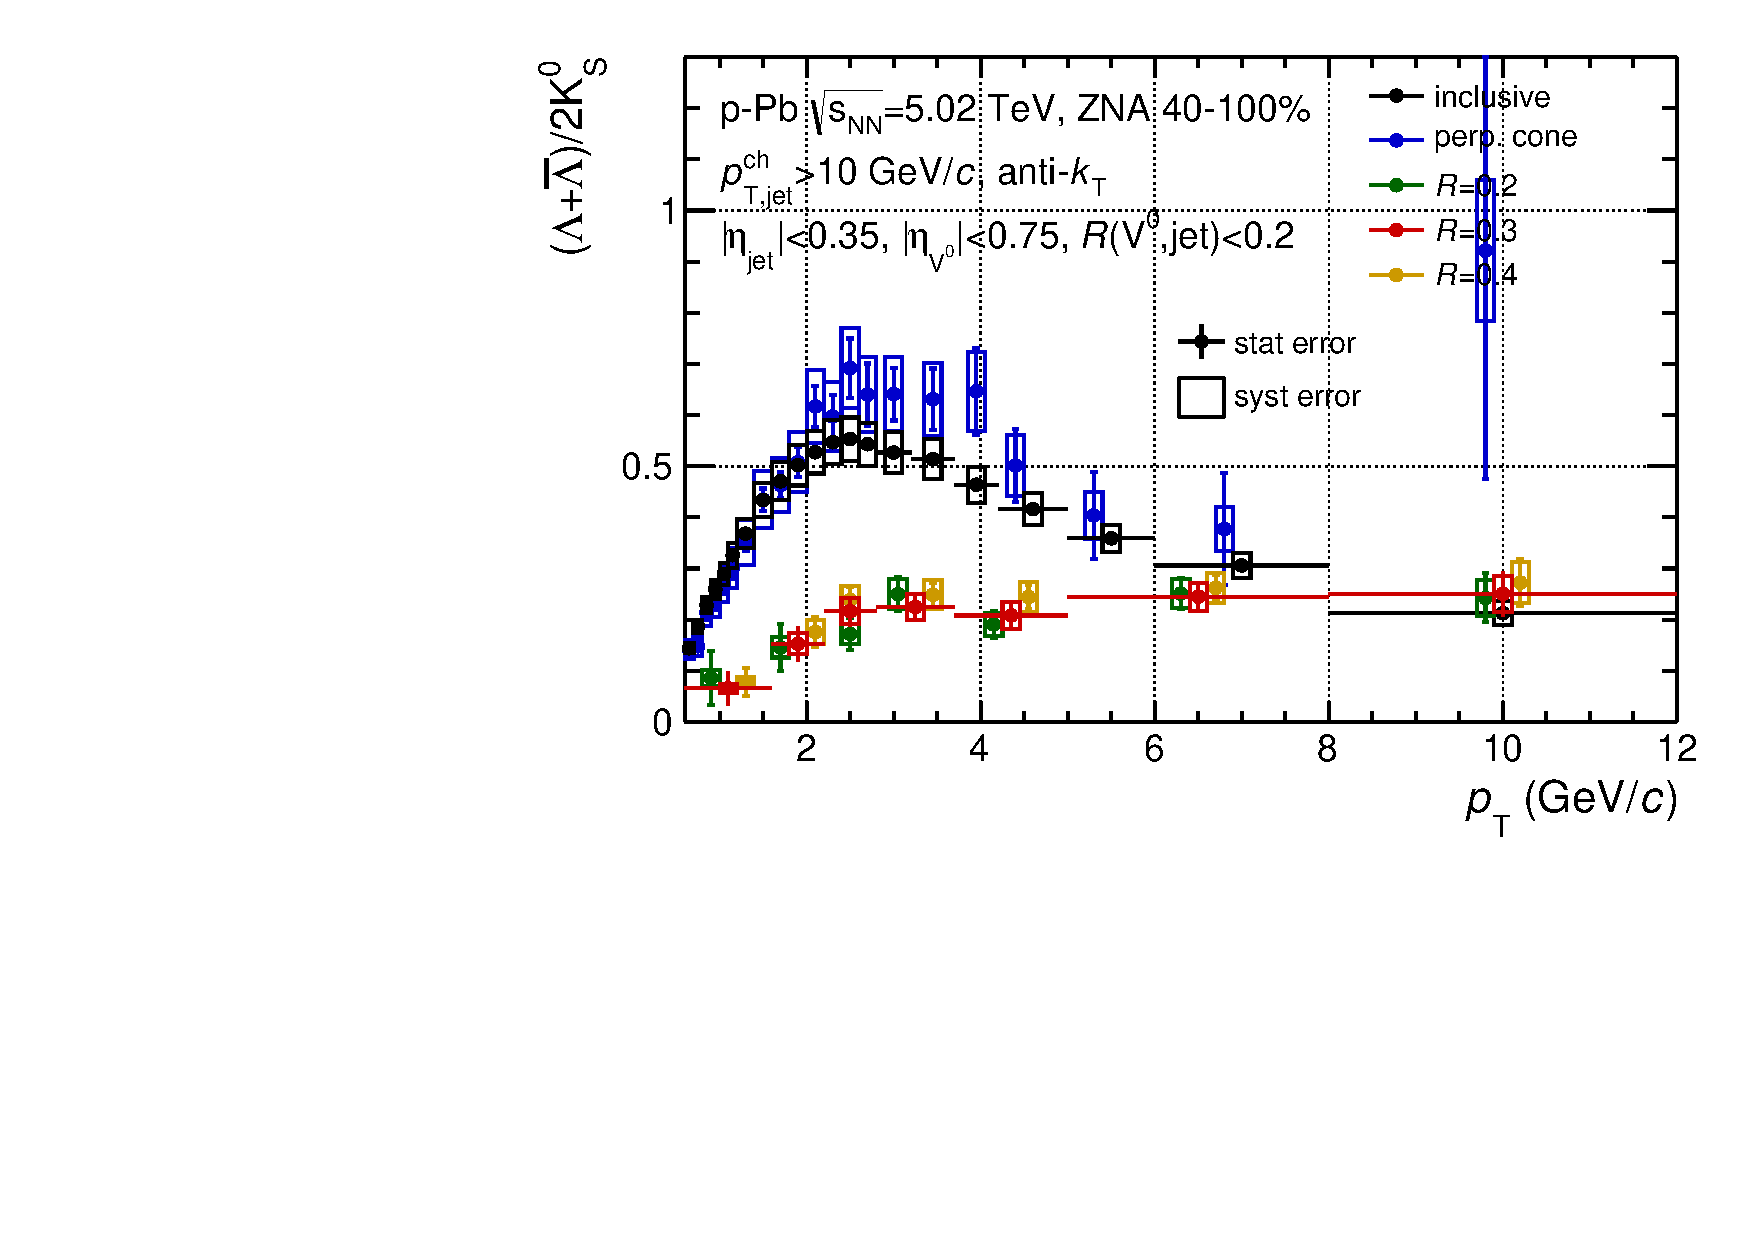
\includegraphics[width=.32\textwidth]{cL2K_Pt_Comp_JC02_ZNA_040_100_PtJ10}
\caption{$\Lambda$-to-$\Kshort$ ratio as a function of $\pT$
  obtained in jets with three different jet resolution
  parameters $R=0.2,~0.3$ and $0.4$ and, $p_{\rm T,jet}>10~\GeVc$.
  The $\Vzero$--jet matching radius $R(\Vzero,{\rm jet})<0.2$.
  Results are shown in three ZNA event activity classes and
  compared with the inclusive and the underlying $\Vzeros$.}
\label{fig:s01L2KJC02ZNAPtj10}
\end{figure}

\begin{figure}[htbp]
\centering
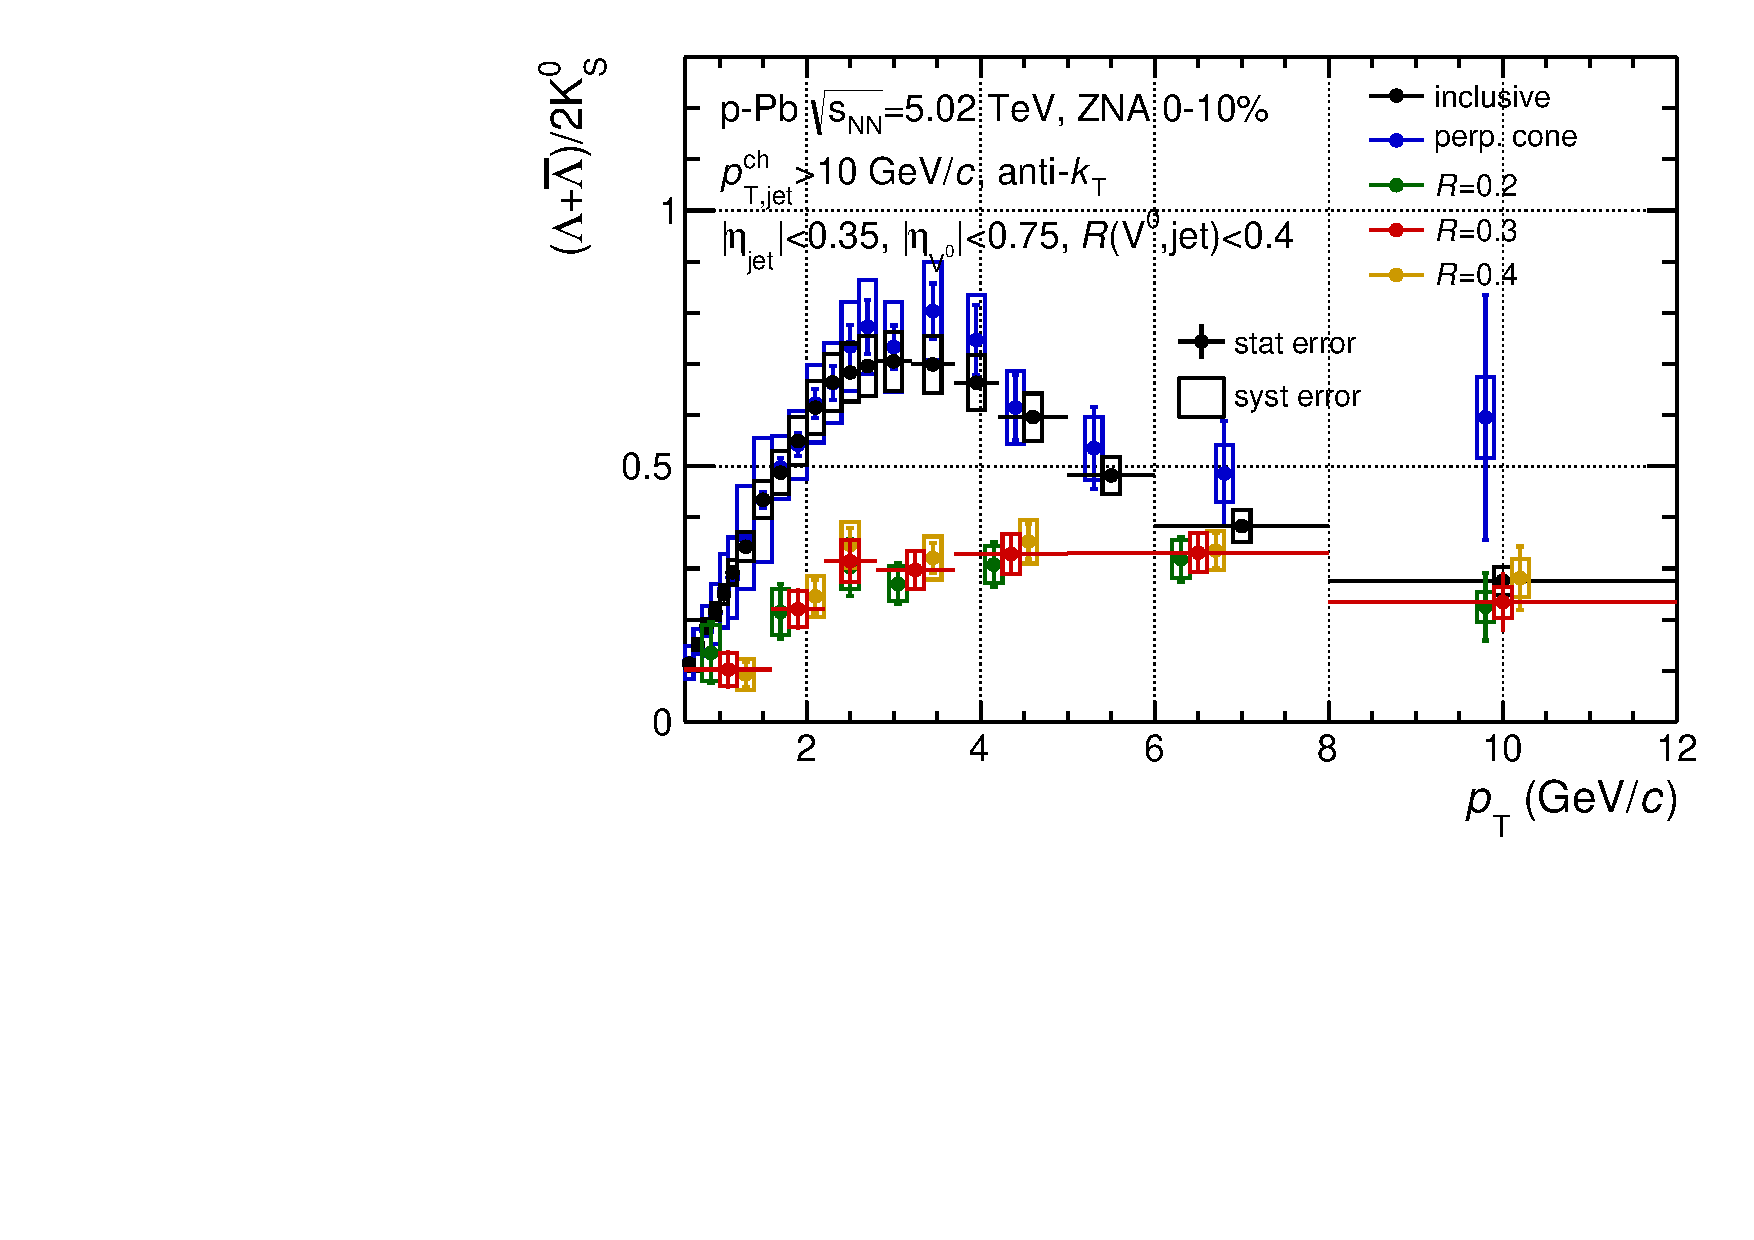
\includegraphics[width=.32\textwidth]{cL2K_Pt_Comp_JC04_ZNA_000_010_PtJ10}
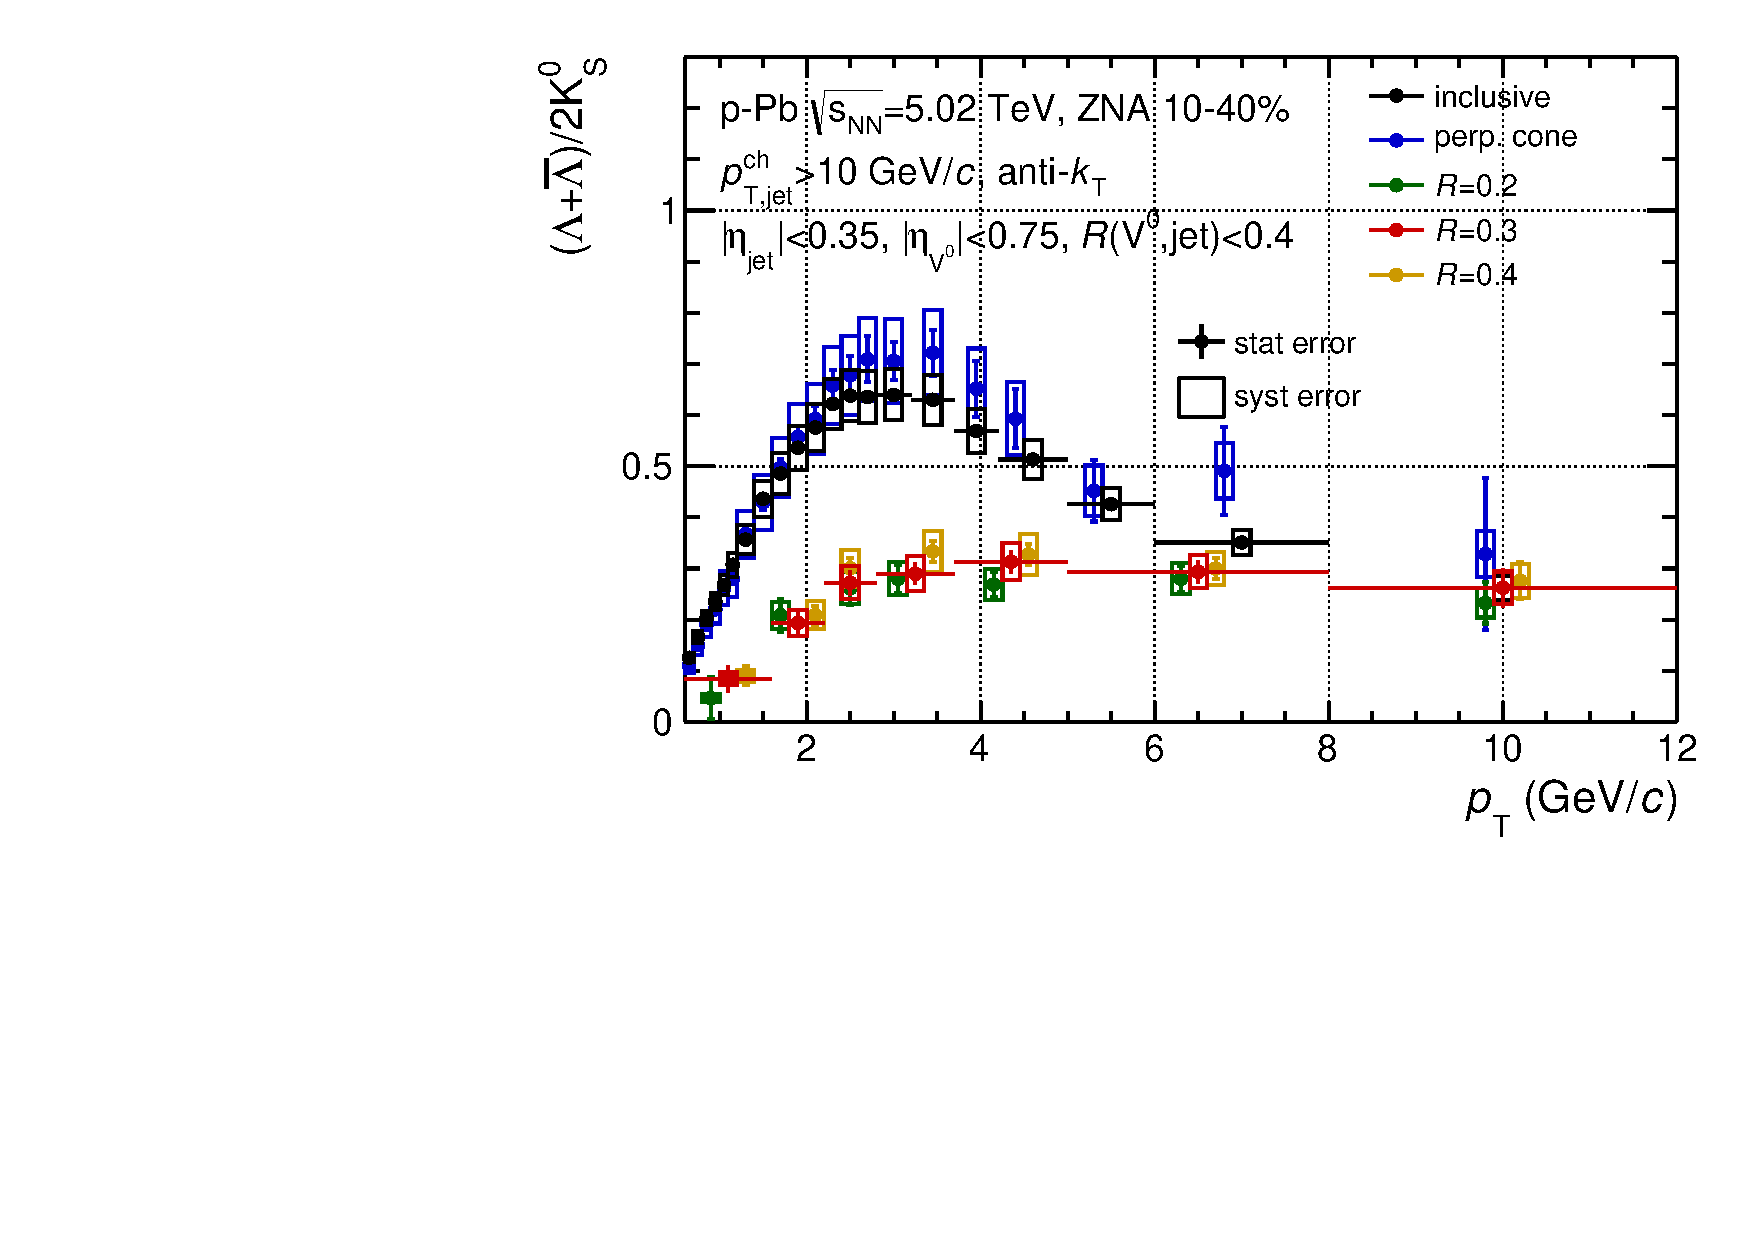
\includegraphics[width=.32\textwidth]{cL2K_Pt_Comp_JC04_ZNA_010_040_PtJ10}
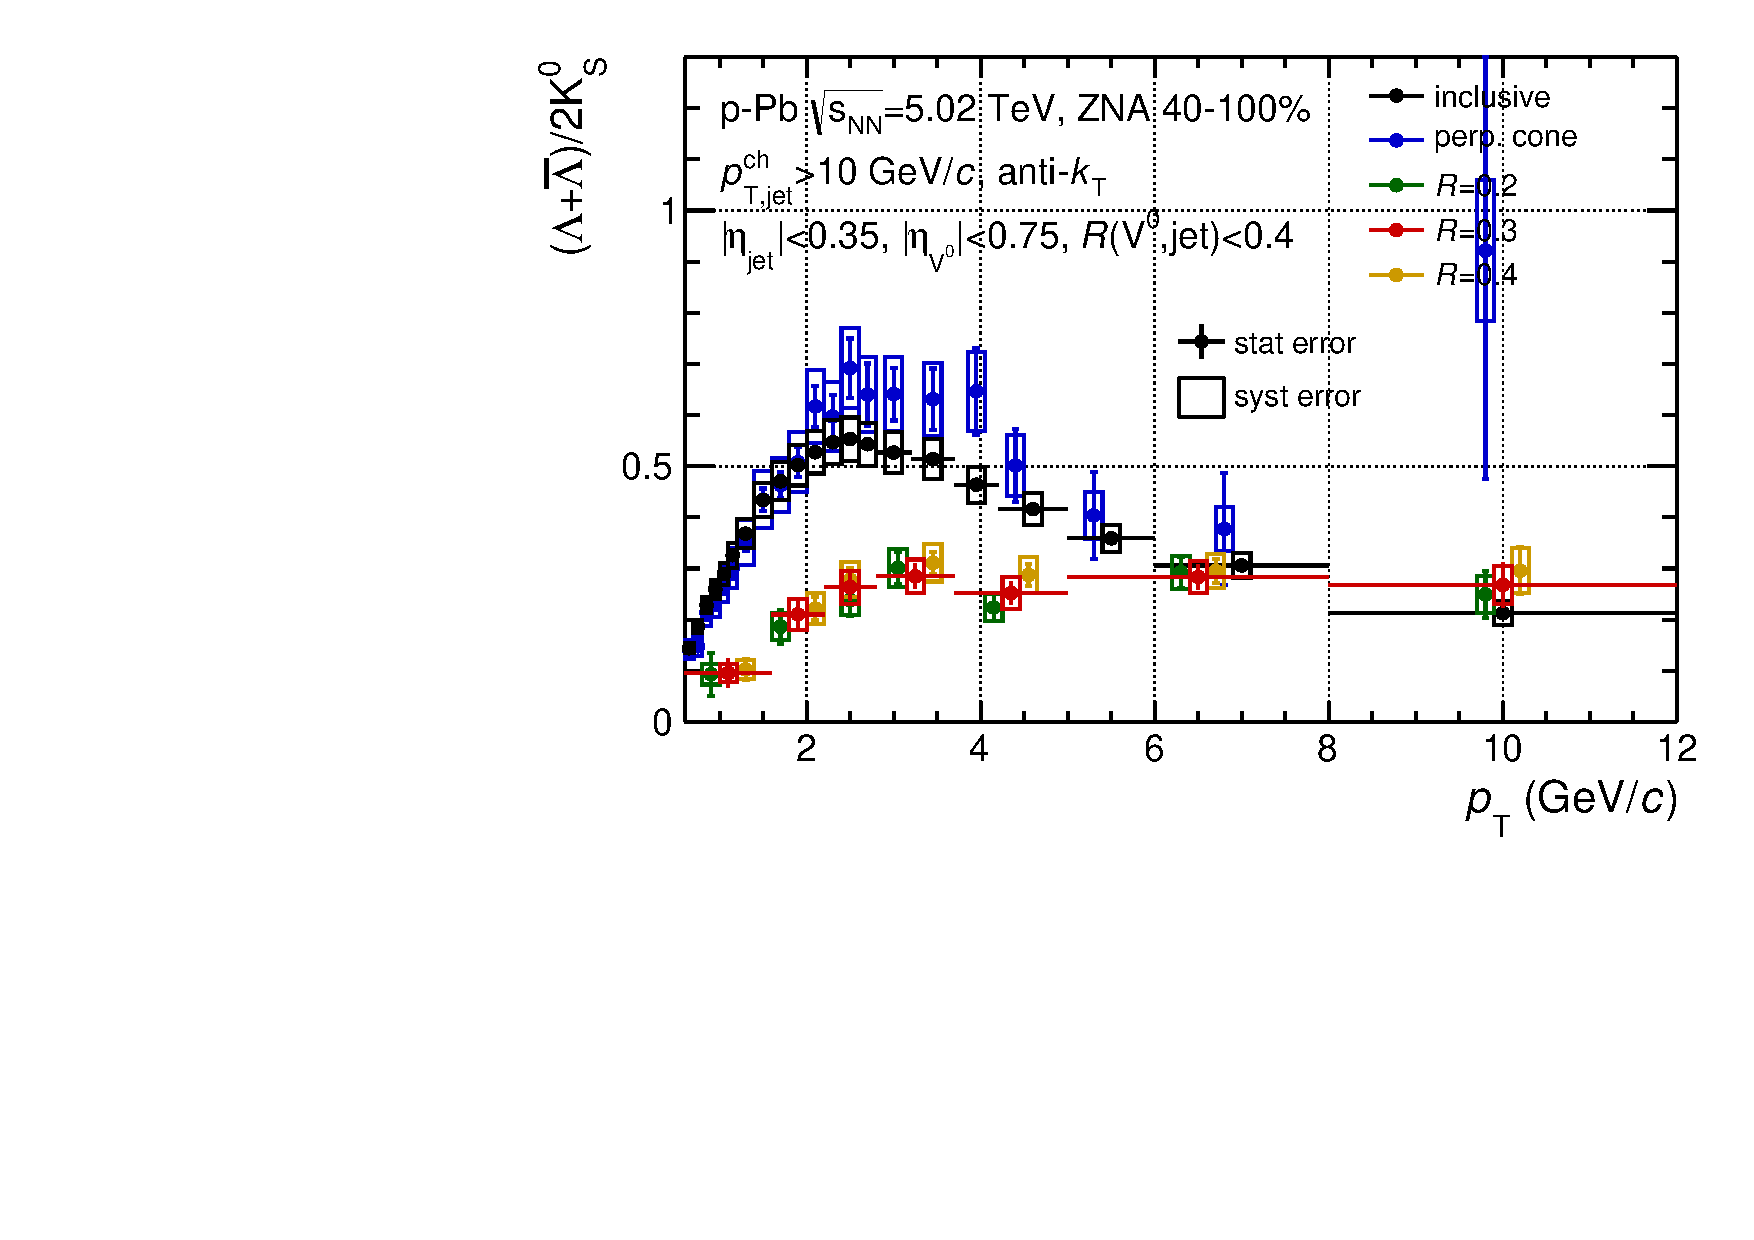
\includegraphics[width=.32\textwidth]{cL2K_Pt_Comp_JC04_ZNA_040_100_PtJ10}
\caption{$\Lambda$-to-$\Kshort$ ratio as a function of $\pT$
  obtained in jets with three different jet resolution
  parameters $R=0.2,~0.3$ and $0.4$ and, $p_{\rm T,jet}>10~\GeVc$.
  The $\Vzero$--jet matching radius $R(\Vzero,{\rm jet})<0.4$.
  Results are shown in three ZNA event activity classes and
  compared with the inclusive and the underlying $\Vzeros$.}
\label{fig:s01L2KJC04ZNAPtj10}
\end{figure}

\begin{figure}[htbp]
\centering
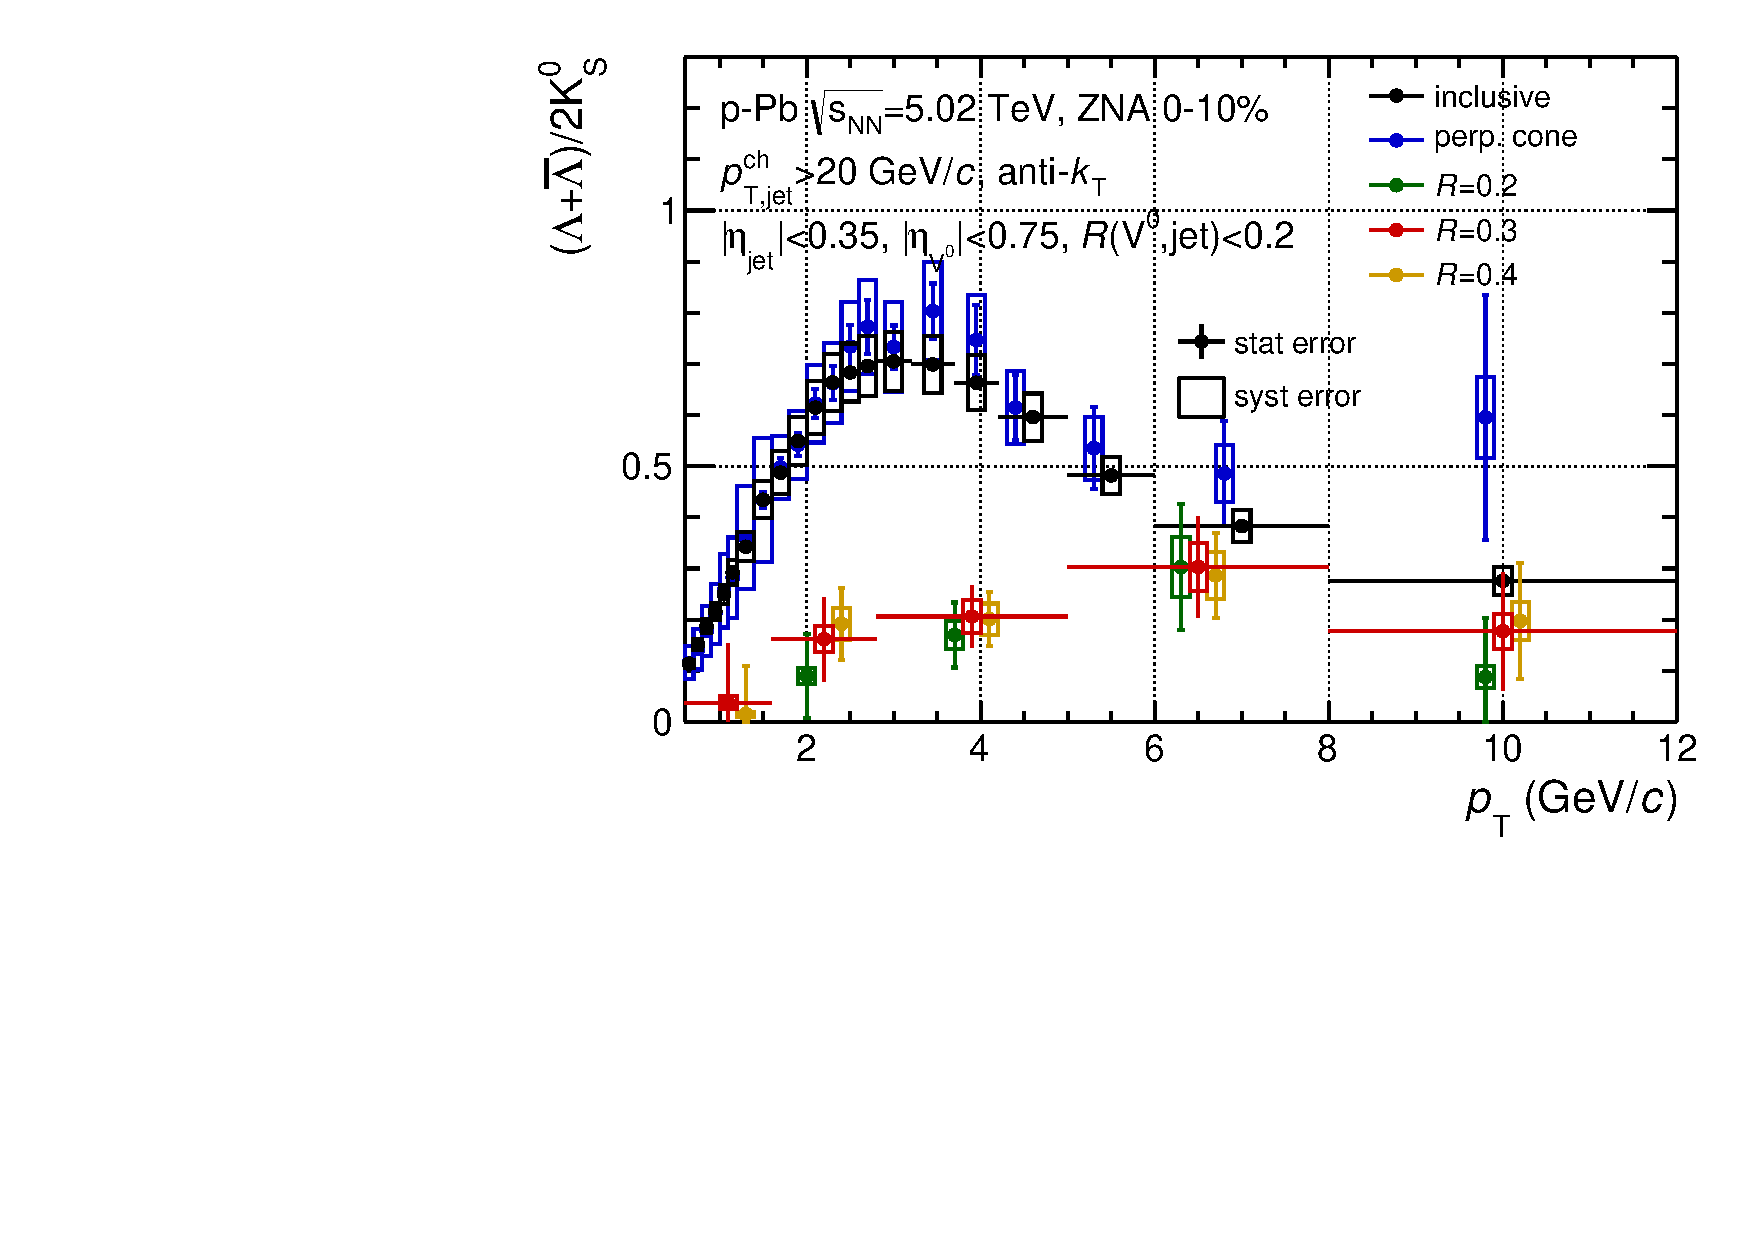
\includegraphics[width=.32\textwidth]{cL2K_Pt_Comp_JC02_ZNA_000_010_PtJ20}
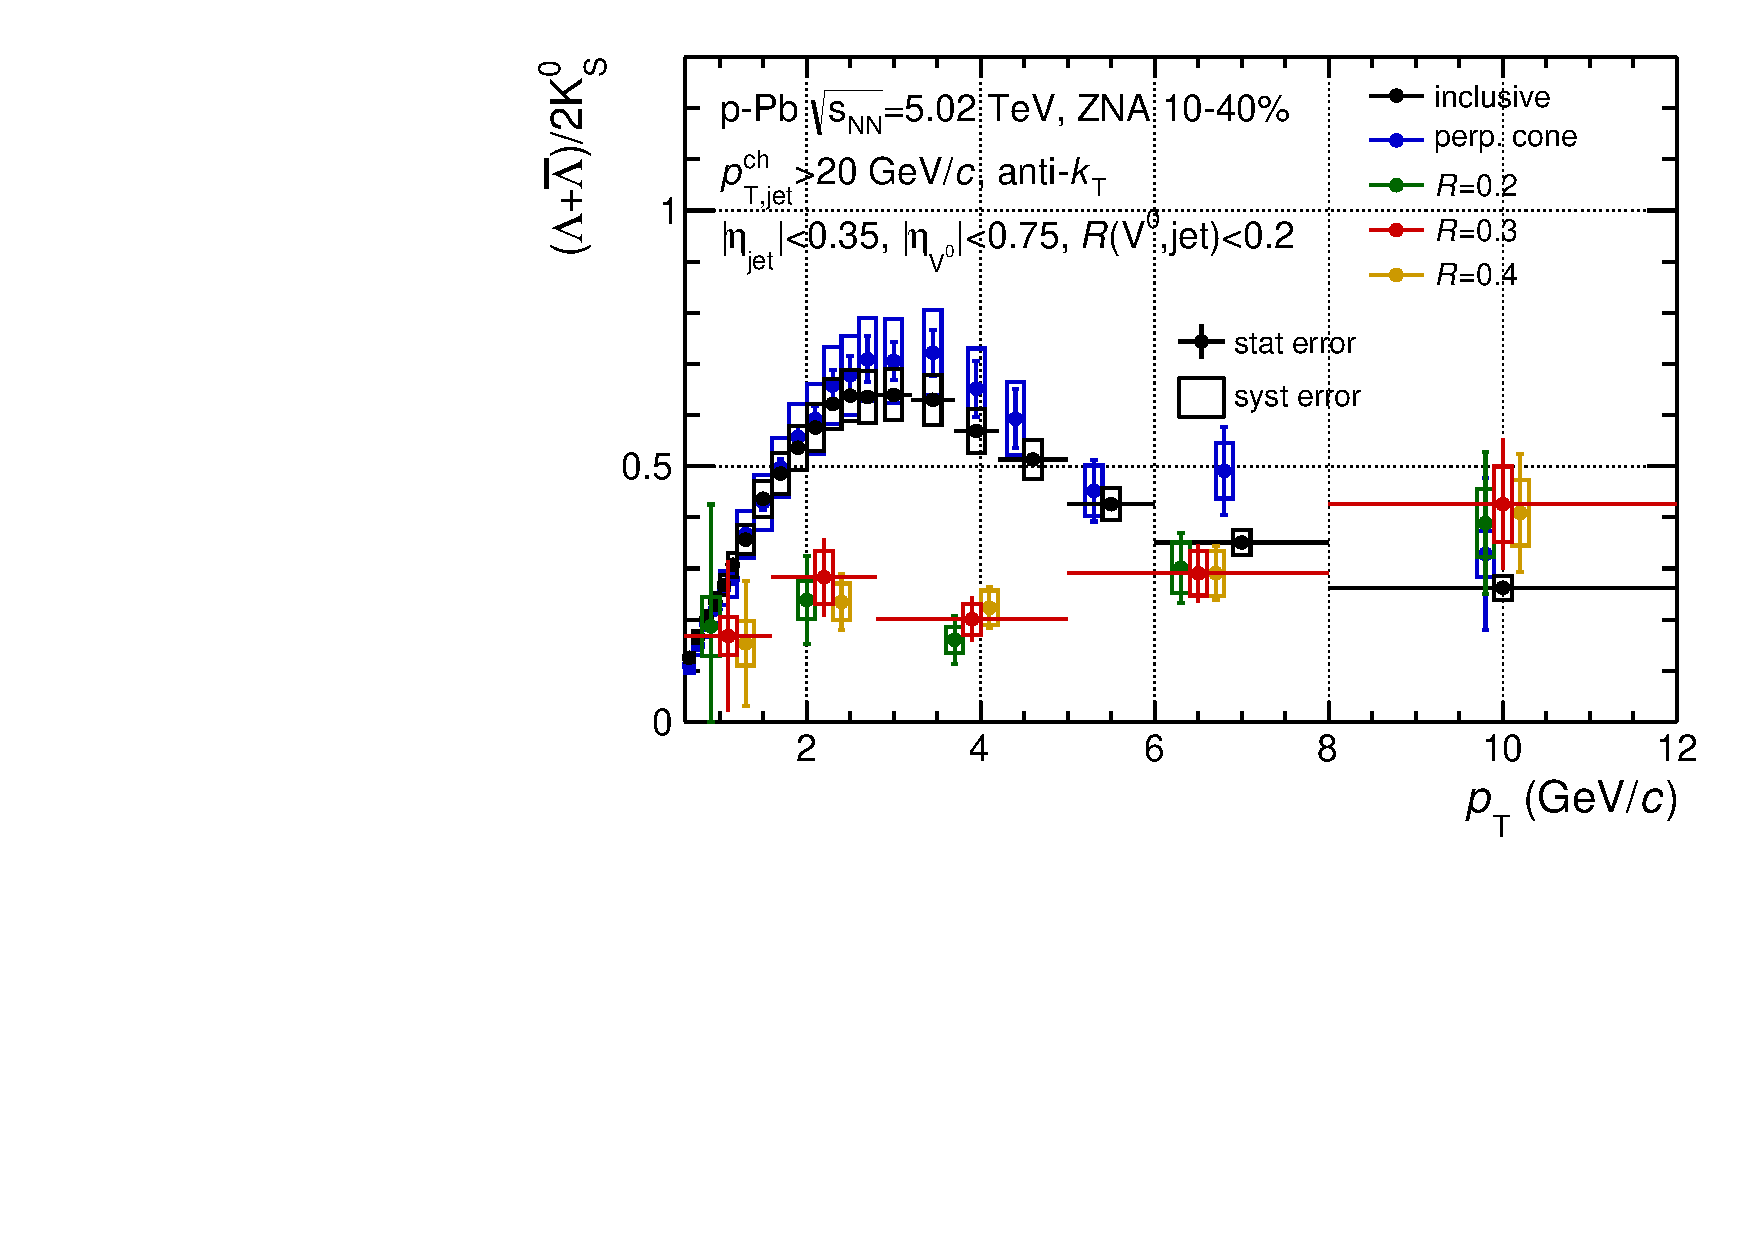
\includegraphics[width=.32\textwidth]{cL2K_Pt_Comp_JC02_ZNA_010_040_PtJ20}
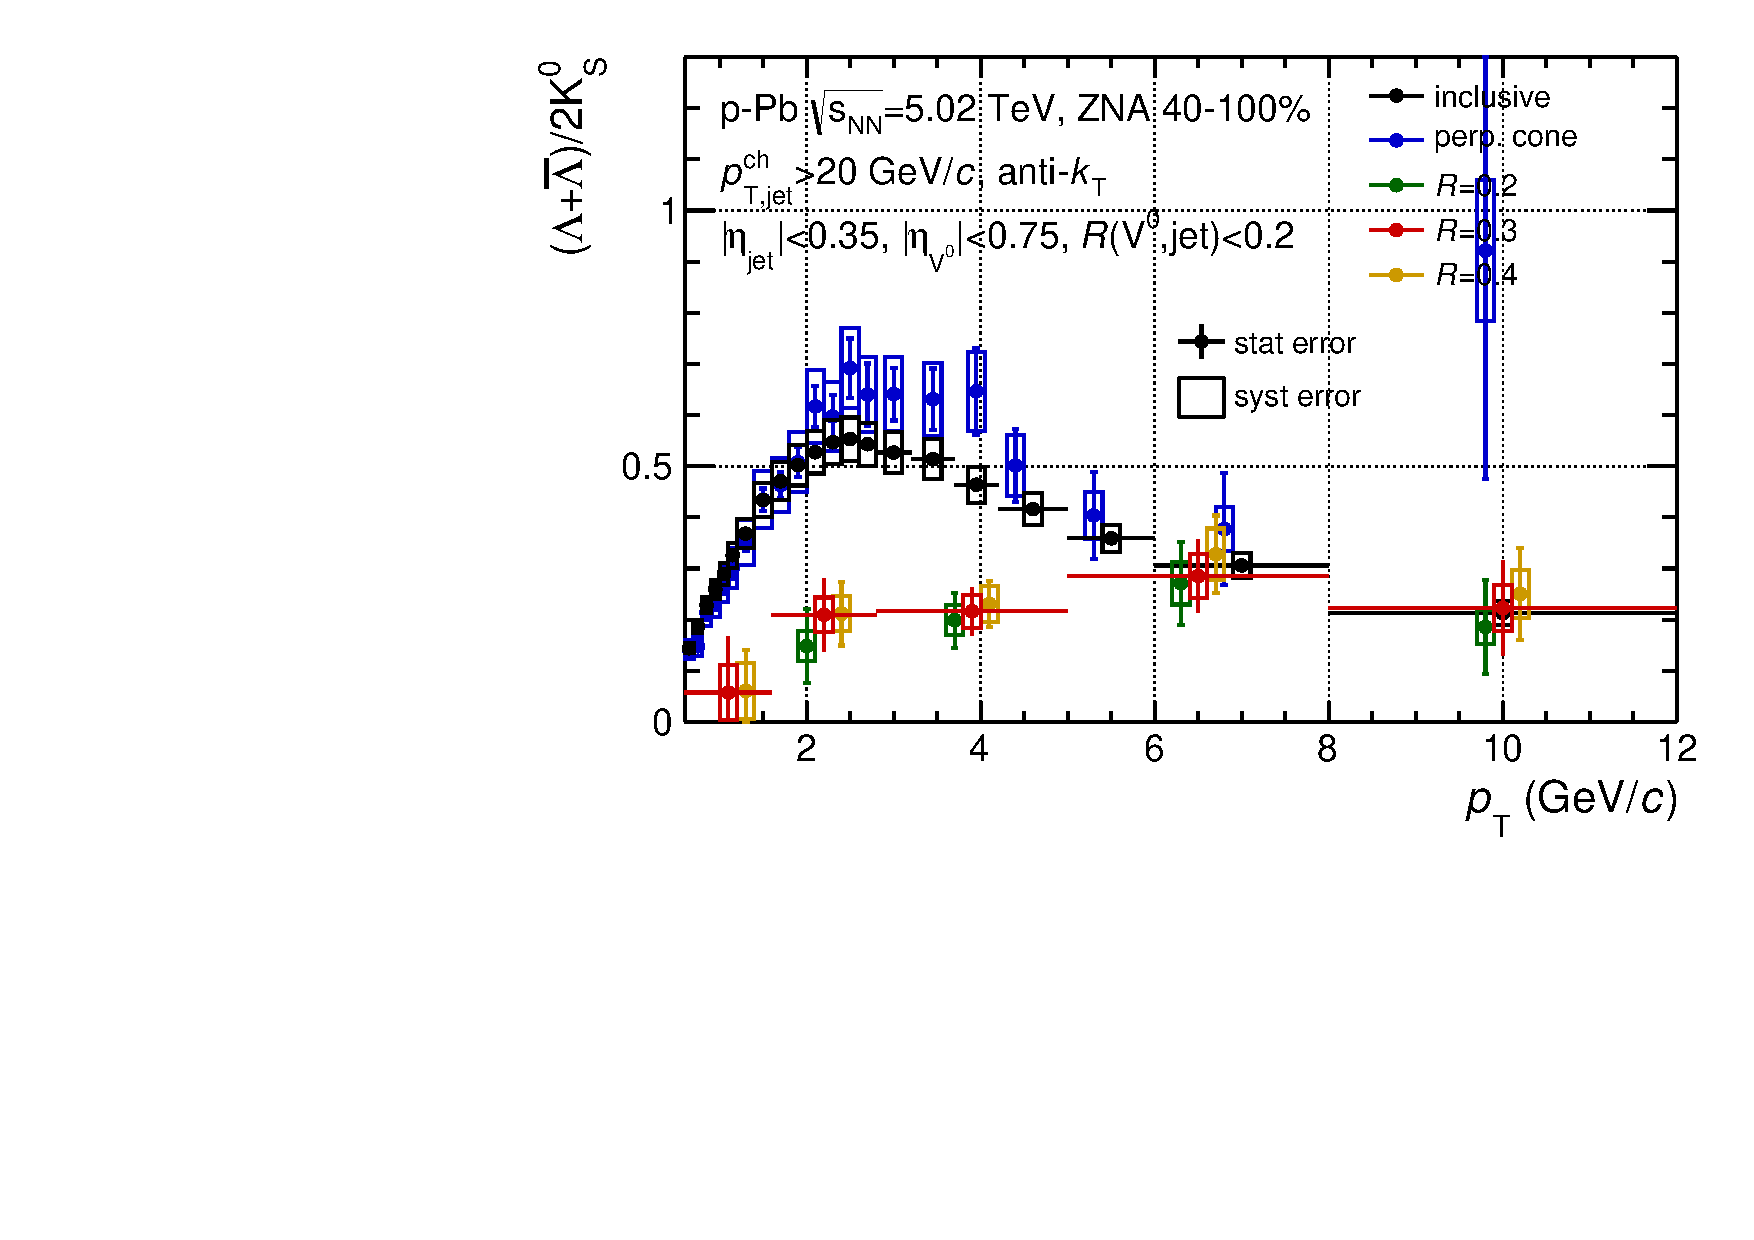
\includegraphics[width=.32\textwidth]{cL2K_Pt_Comp_JC02_ZNA_040_100_PtJ20}
\caption{$\Lambda$-to-$\Kshort$ ratio as a function of $\pT$
  obtained in jets with three different jet resolution
  parameters $R=0.2,~0.3$ and $0.4$ and, $p_{\rm T,jet}>20~\GeVc$.
  The $\Vzero$--jet matching radius $R(\Vzero,{\rm jet})<0.2$.
  Results are shown in three ZNA event activity classes and
  compared with the inclusive and the underlying $\Vzeros$.}
\label{fig:s01L2KJC02ZNAPtj20}
\end{figure}

\begin{figure}[htbp]
\centering
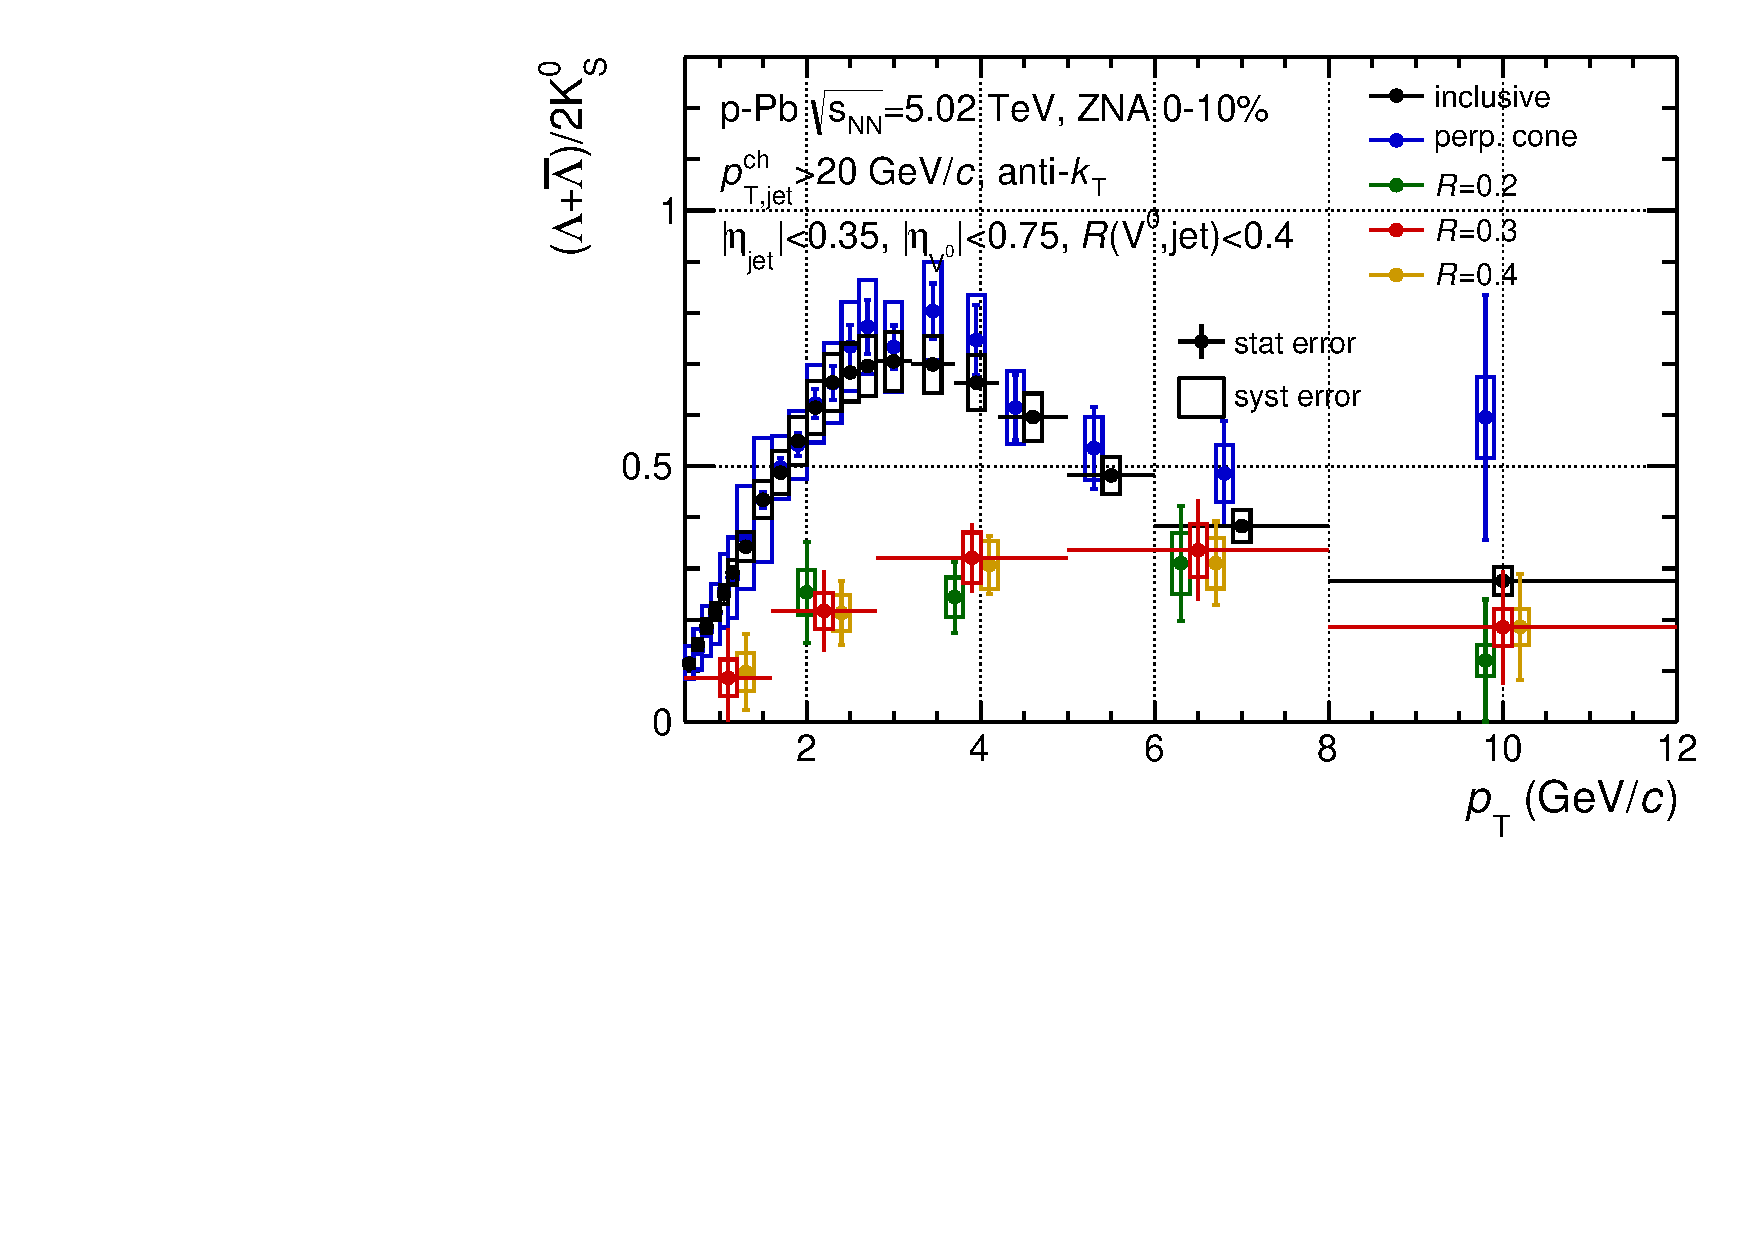
\includegraphics[width=.32\textwidth]{cL2K_Pt_Comp_JC04_ZNA_000_010_PtJ20}
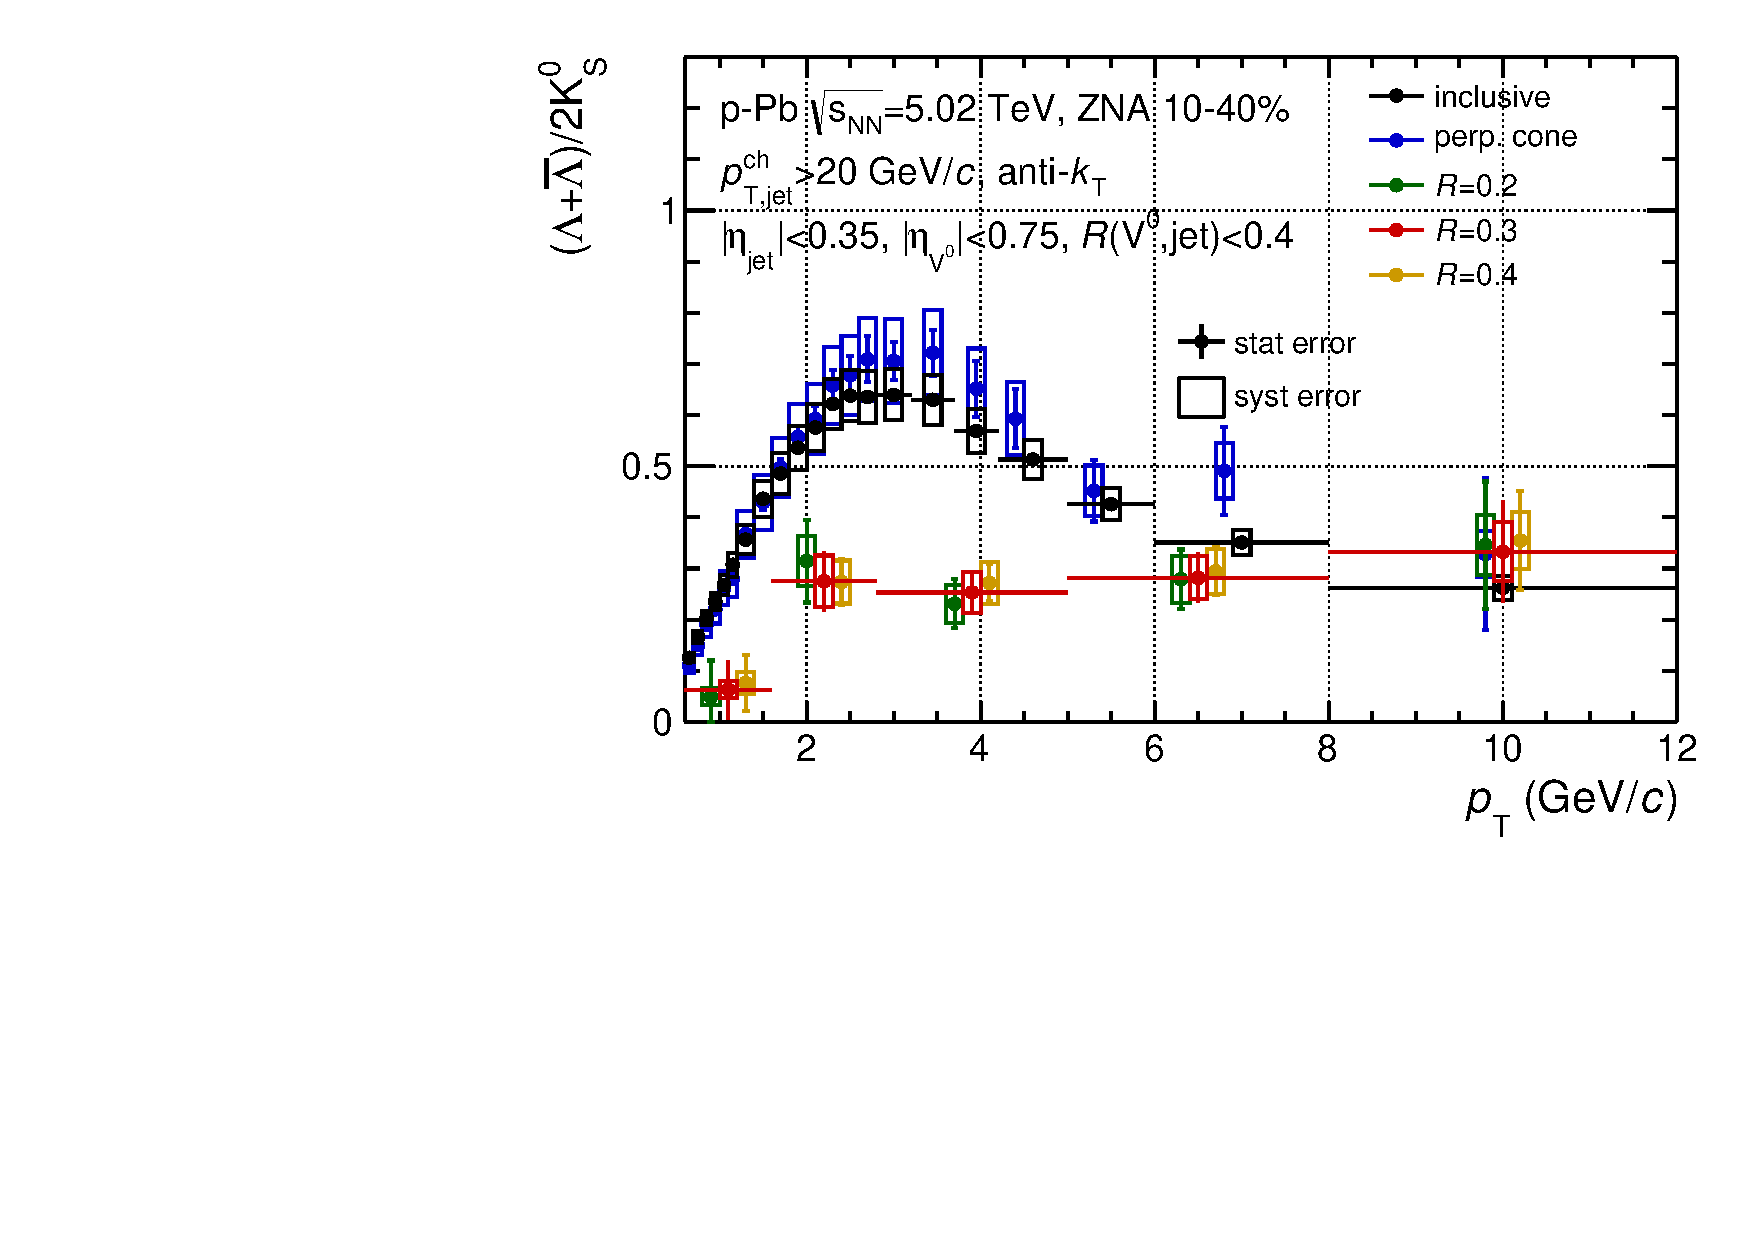
\includegraphics[width=.32\textwidth]{cL2K_Pt_Comp_JC04_ZNA_010_040_PtJ20}
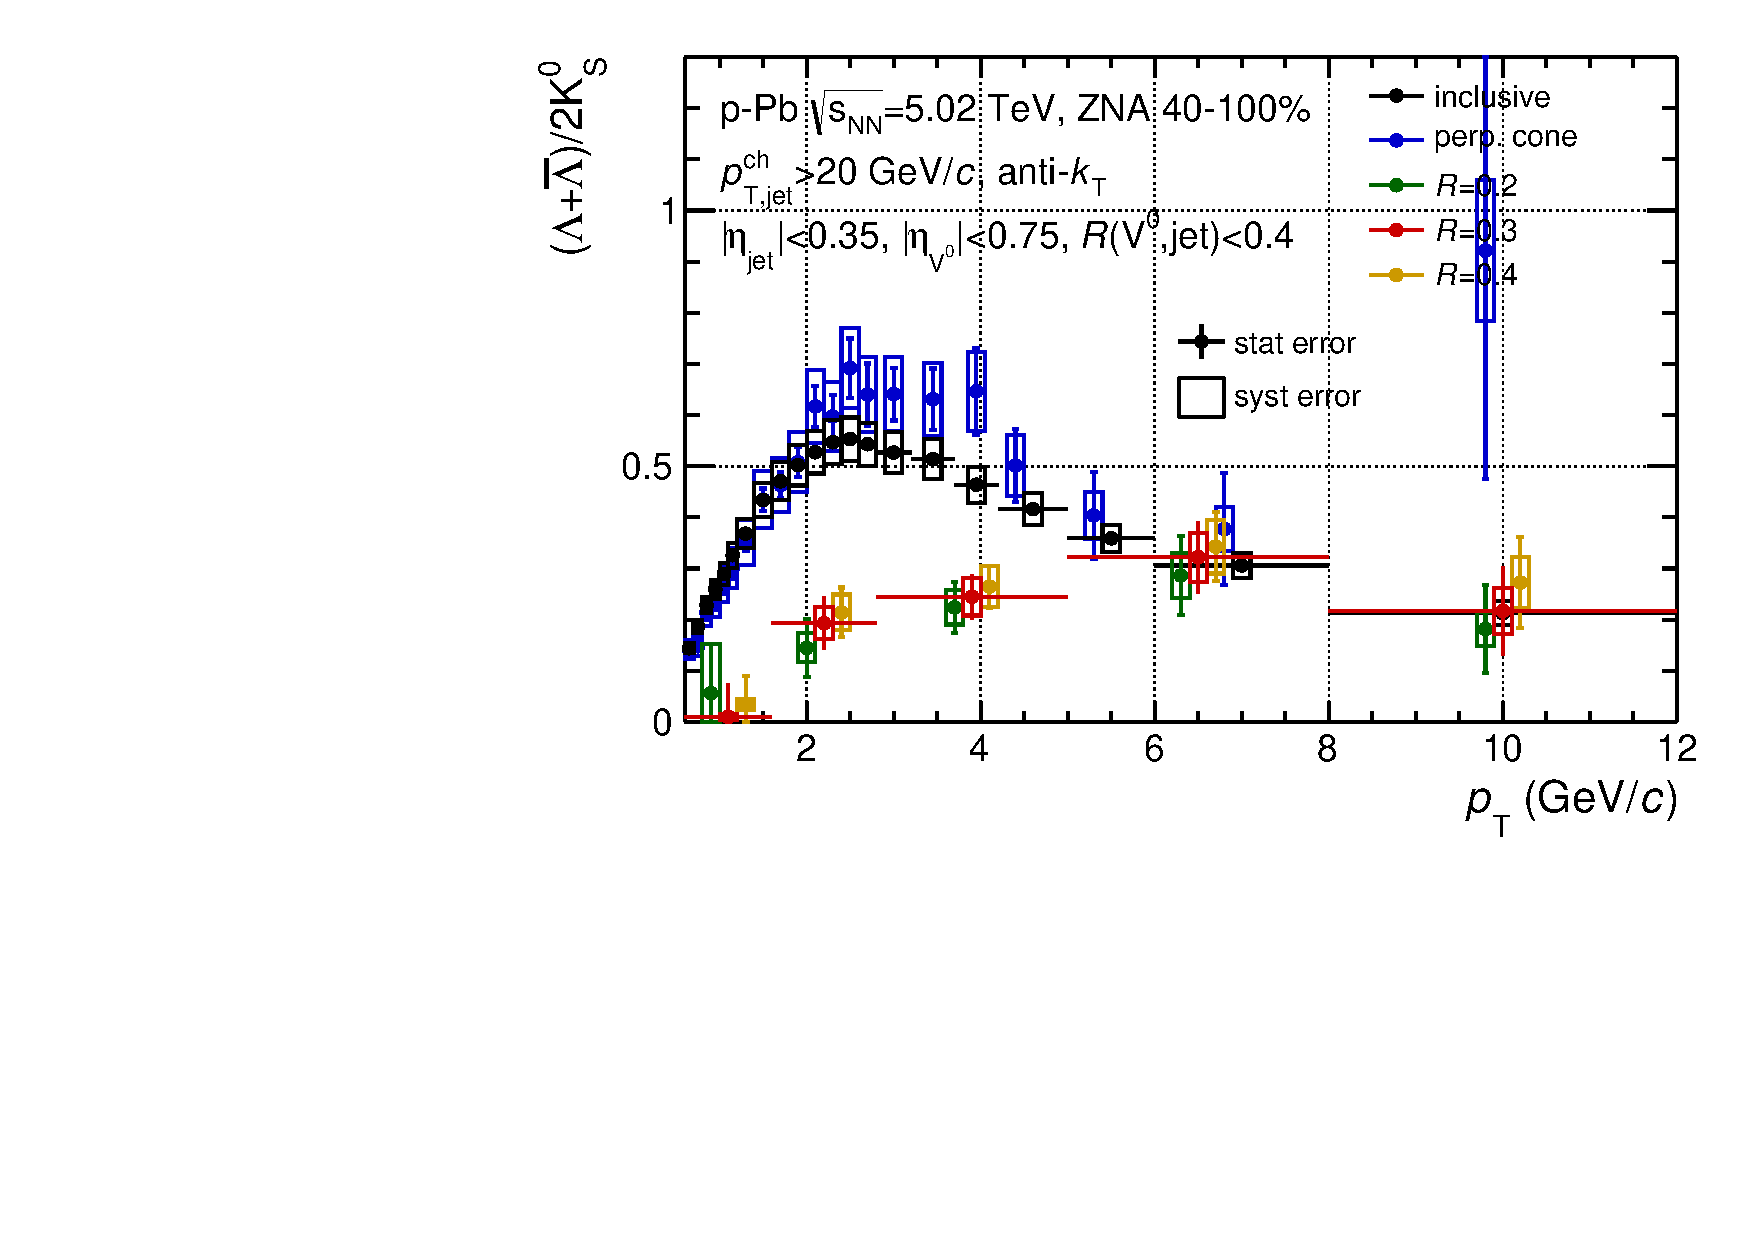
\includegraphics[width=.32\textwidth]{cL2K_Pt_Comp_JC04_ZNA_040_100_PtJ20}
\caption{$\Lambda$-to-$\Kshort$ ratio as a function of $\pT$
  obtained in jets with three different jet resolution
  parameters $R=0.2,~0.3$ and $0.4$ and, $p_{\rm T,jet}>20~\GeVc$.
  The $\Vzero$--jet matching radius $R(\Vzero,{\rm jet})<0.4$.
  Results are shown in three ZNA event activity classes and
  compared with the inclusive and the underlying $\Vzeros$.}
\label{fig:s01L2KJC04ZNAPtj20}
\end{figure}
%%%%%%%%%%%%%%%%%%%%%%%%%%%%%%%%%%%%%%%%%%%%%%%%%%%%%%%%%%%%%%%%%%%%%%%%%%%%%%%

\newpage
\subsection{$\Lambda$-to-$\Kshort$ ratio in jets averaged over $R=0.2,~0.3$ and $0.4$}

\subsubsection{V0A Event Activity Estimator}

\begin{figure}[htbp]
\centering
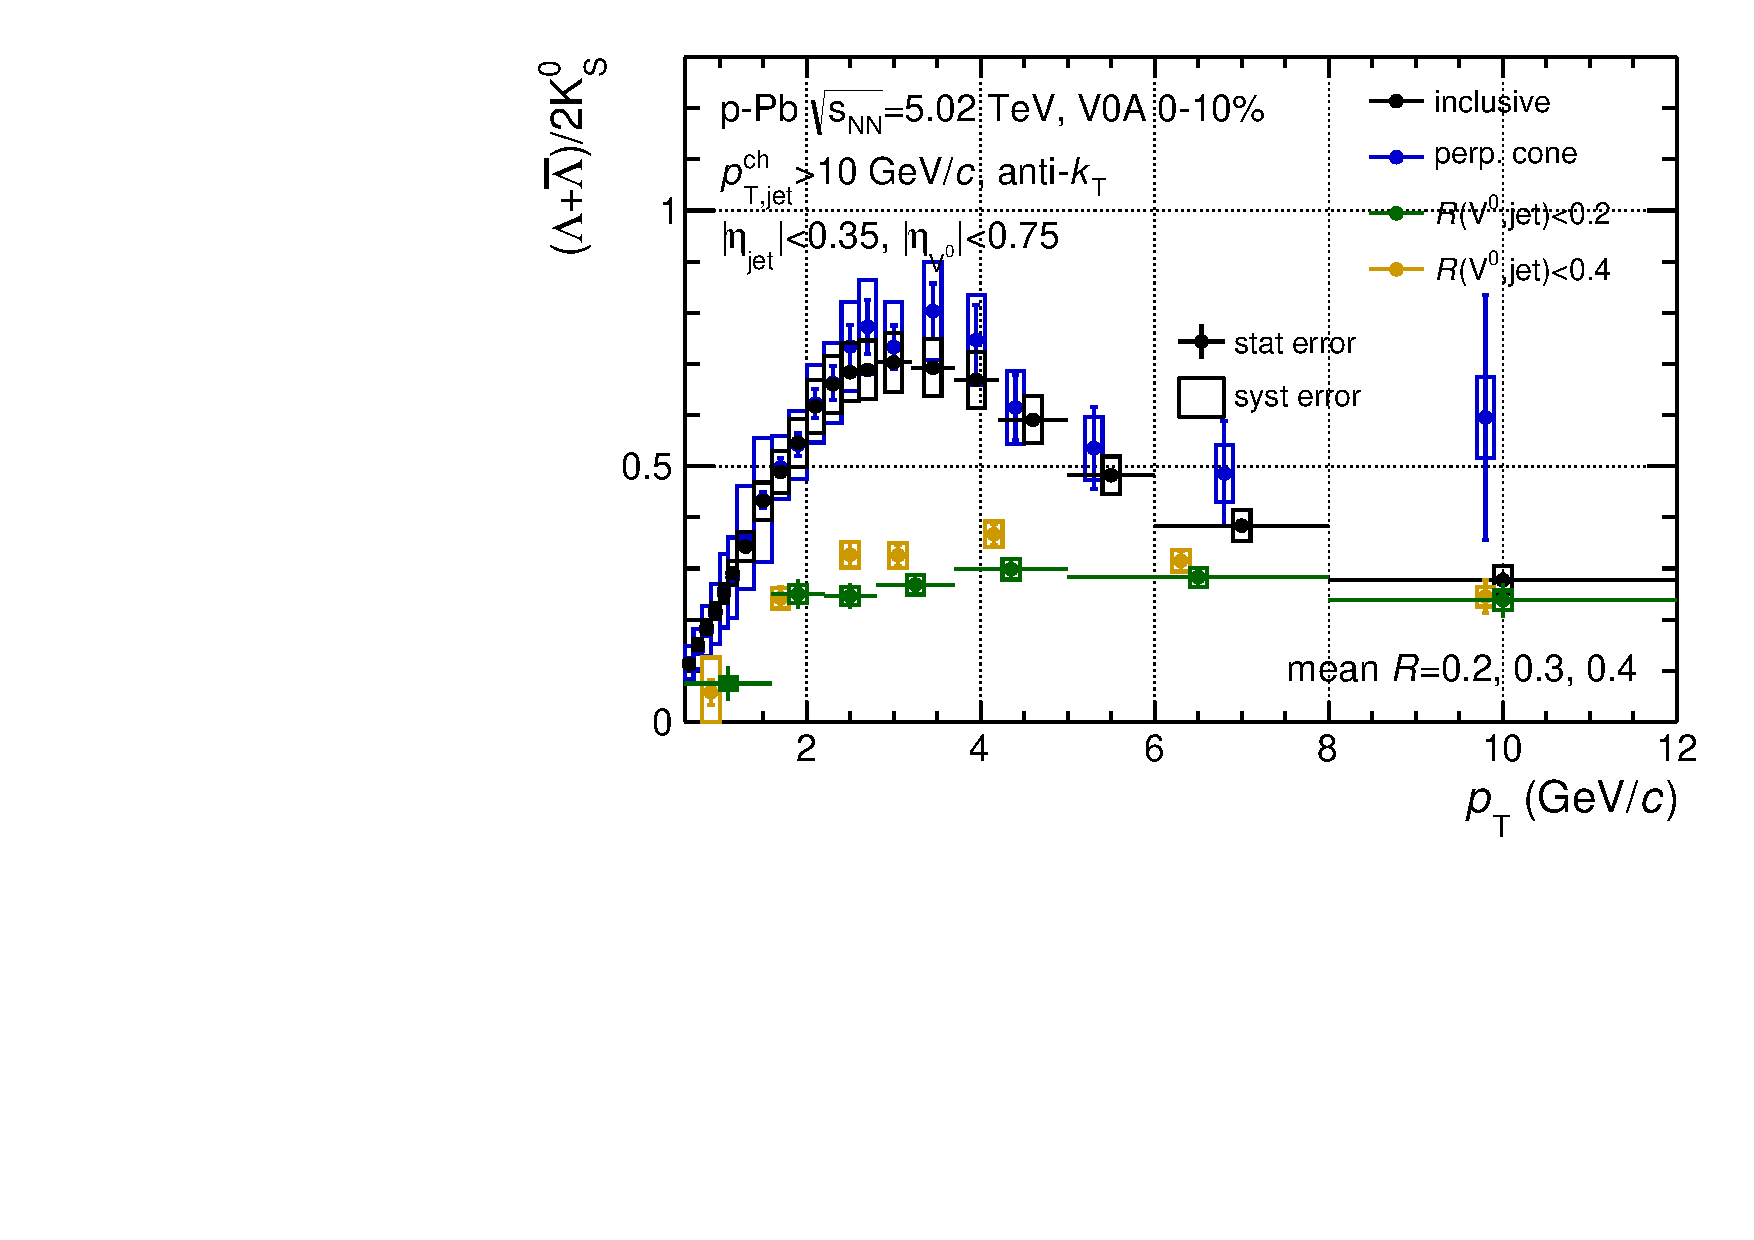
\includegraphics[width=.32\textwidth]{cL2K_Pt_Mean_V0A_000_010_PtJ10}
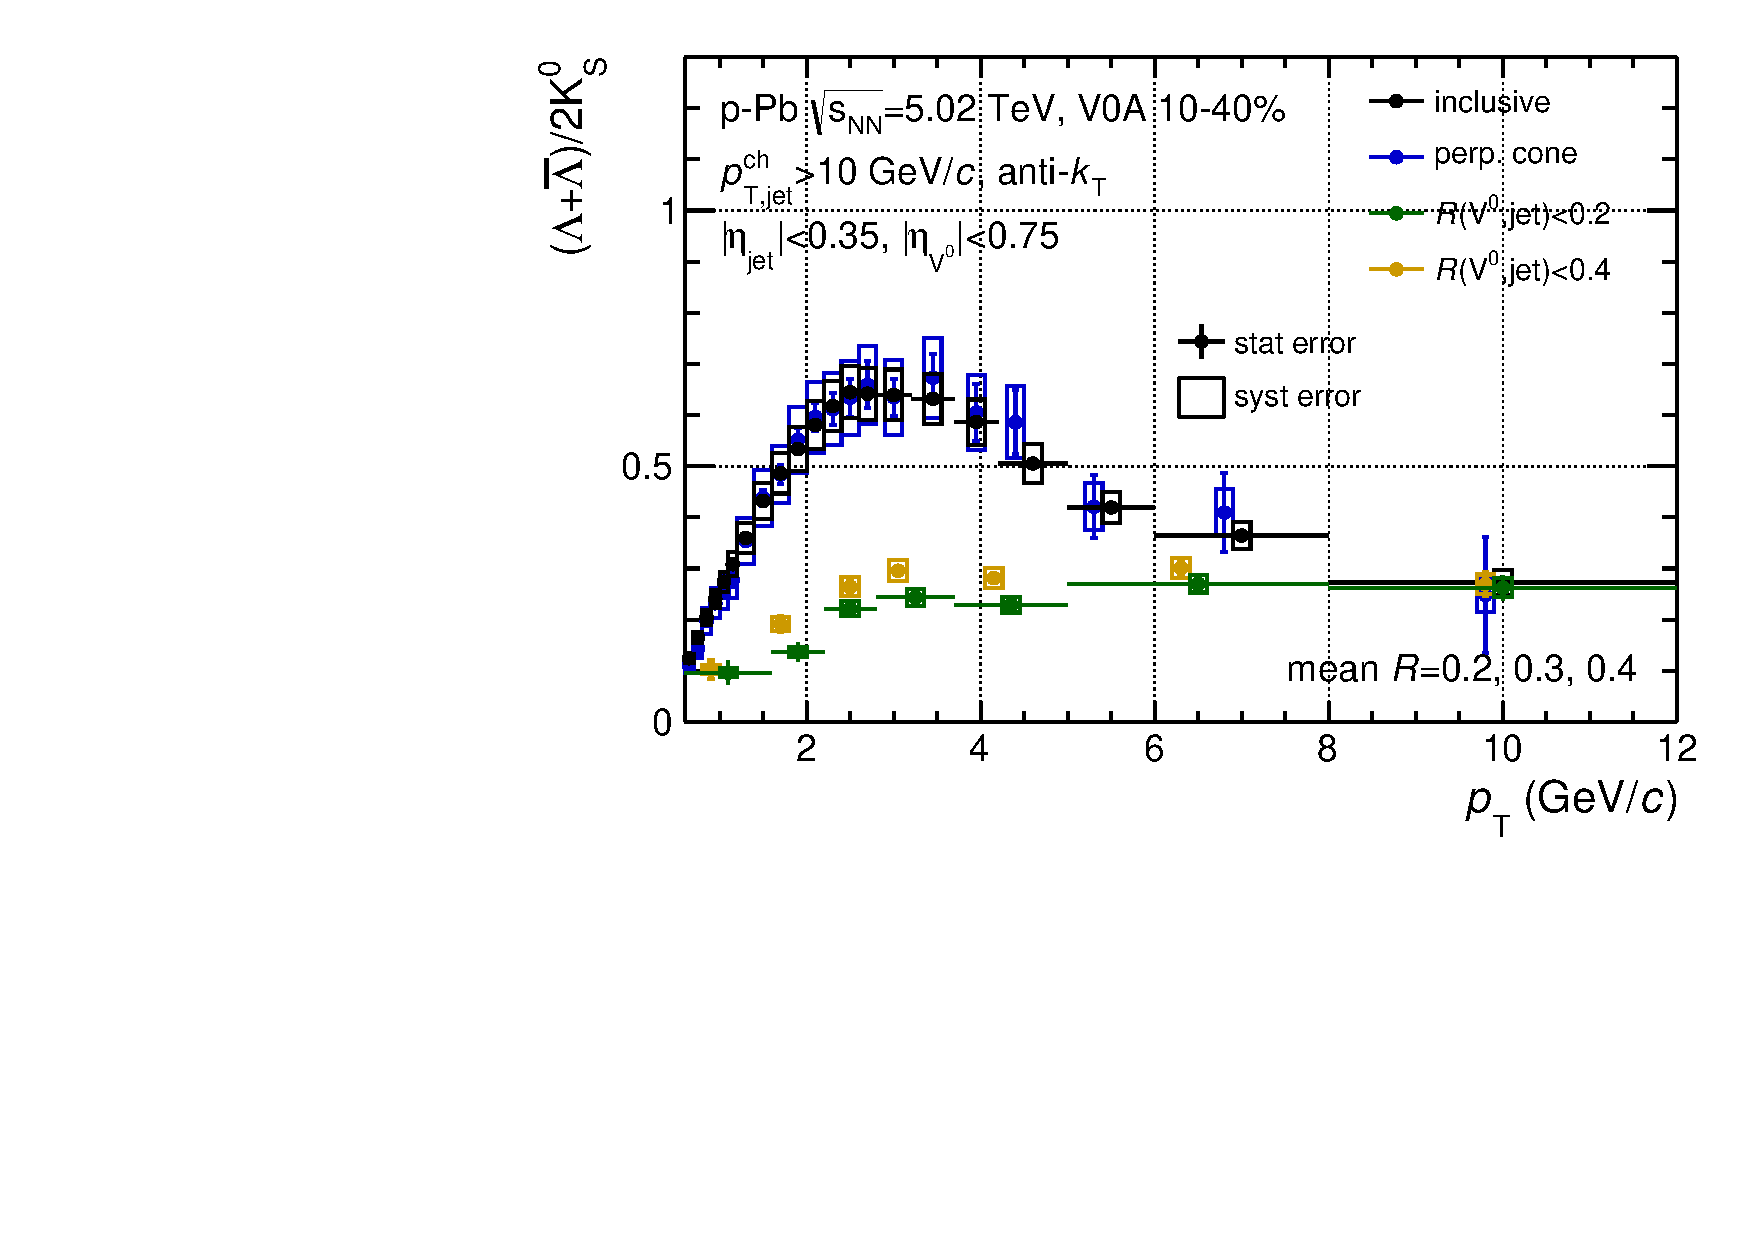
\includegraphics[width=.32\textwidth]{cL2K_Pt_Mean_V0A_010_040_PtJ10}
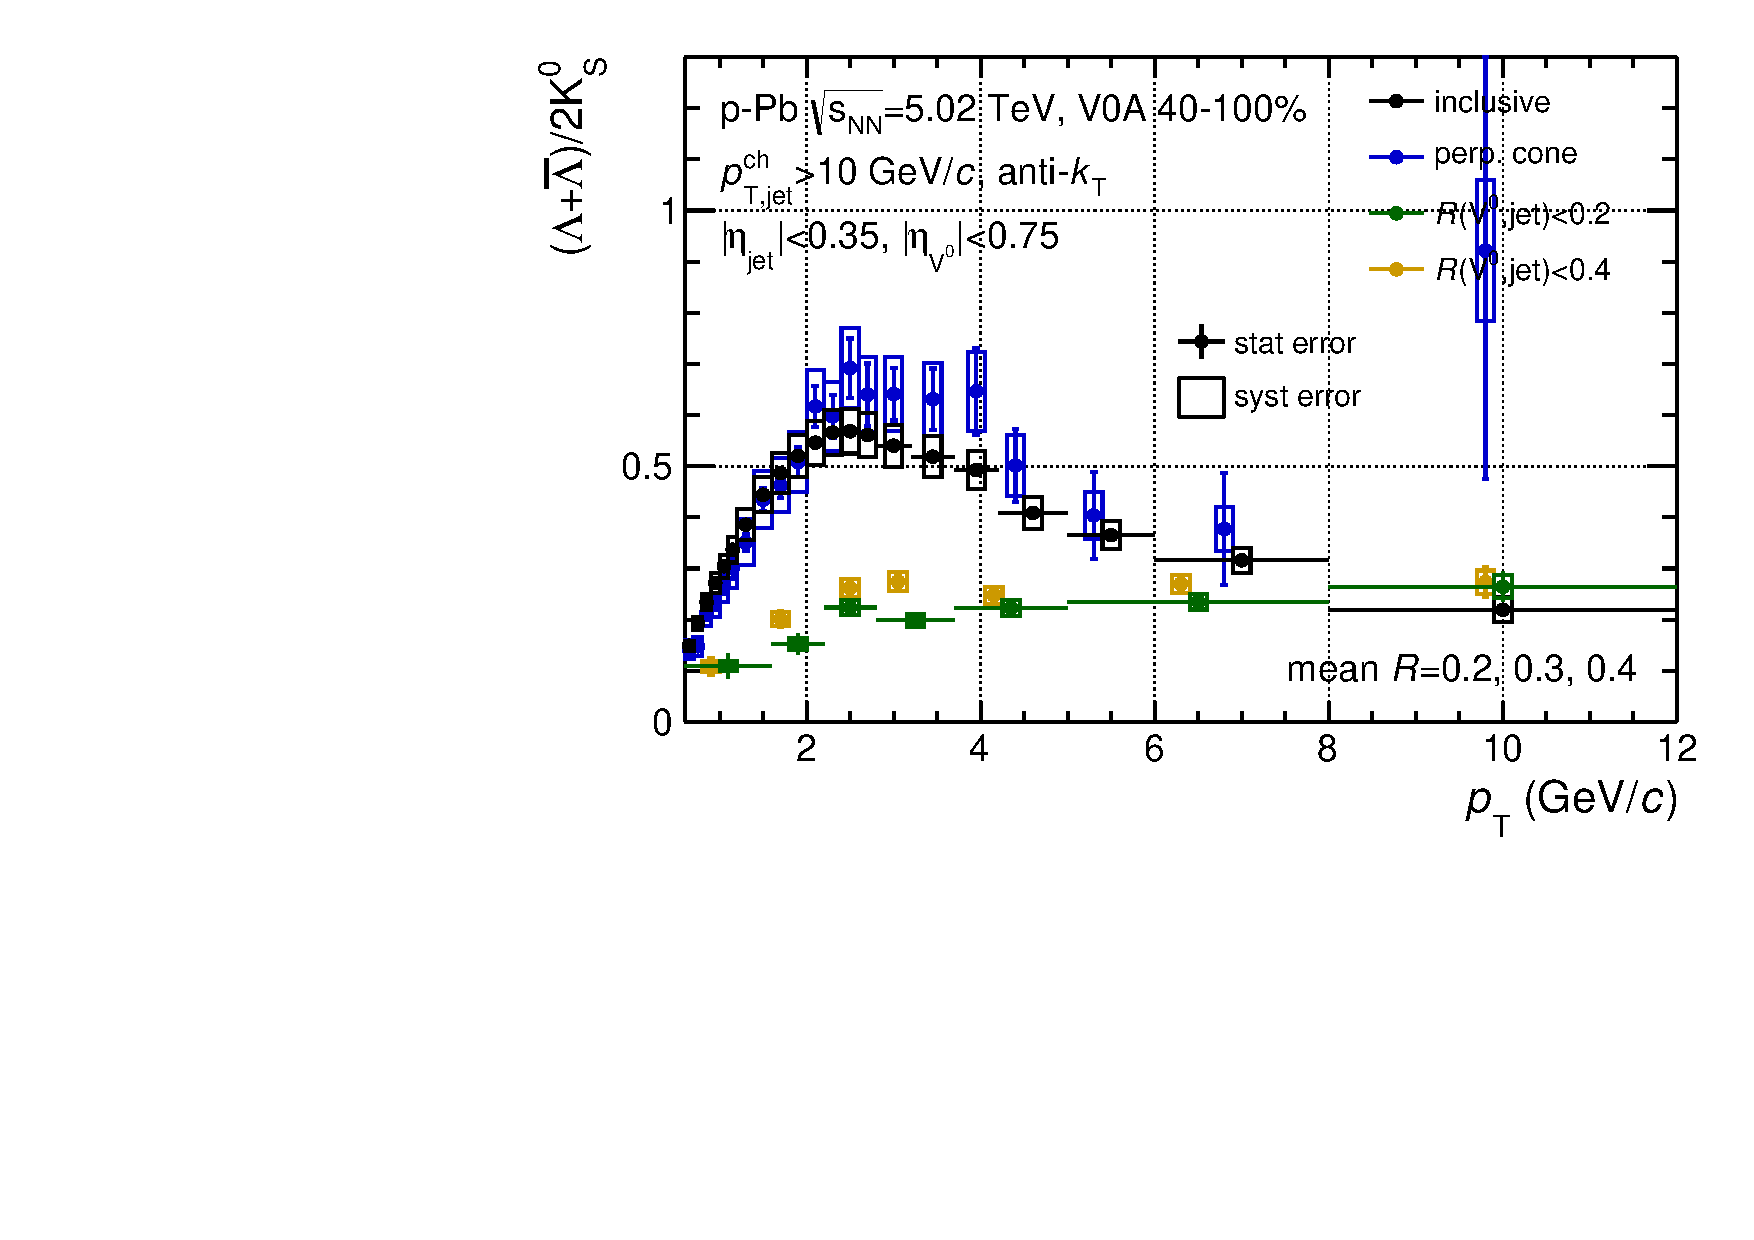
\includegraphics[width=.32\textwidth]{cL2K_Pt_Mean_V0A_040_100_PtJ10}
\caption{$\Lambda$-to-$\Kshort$ ratio as a function of $\pT$
  averaged over jets with
  $R=0.2,~0.3$ and $0.4$ in $p_{\rm T,jet}>10~\GeVc$.
  Two $\Vzero$--jet matching radii $R(\Vzero,{\rm jet})<0.2$ and $0.4$ are used.
  Results are shown in three V0A event activity classes and
  compared with the inclusive and the underlying $\Vzeros$.}
\label{fig:s01L2KJC0XV0APtj10}
\end{figure}

\begin{figure}[htbp]
\centering
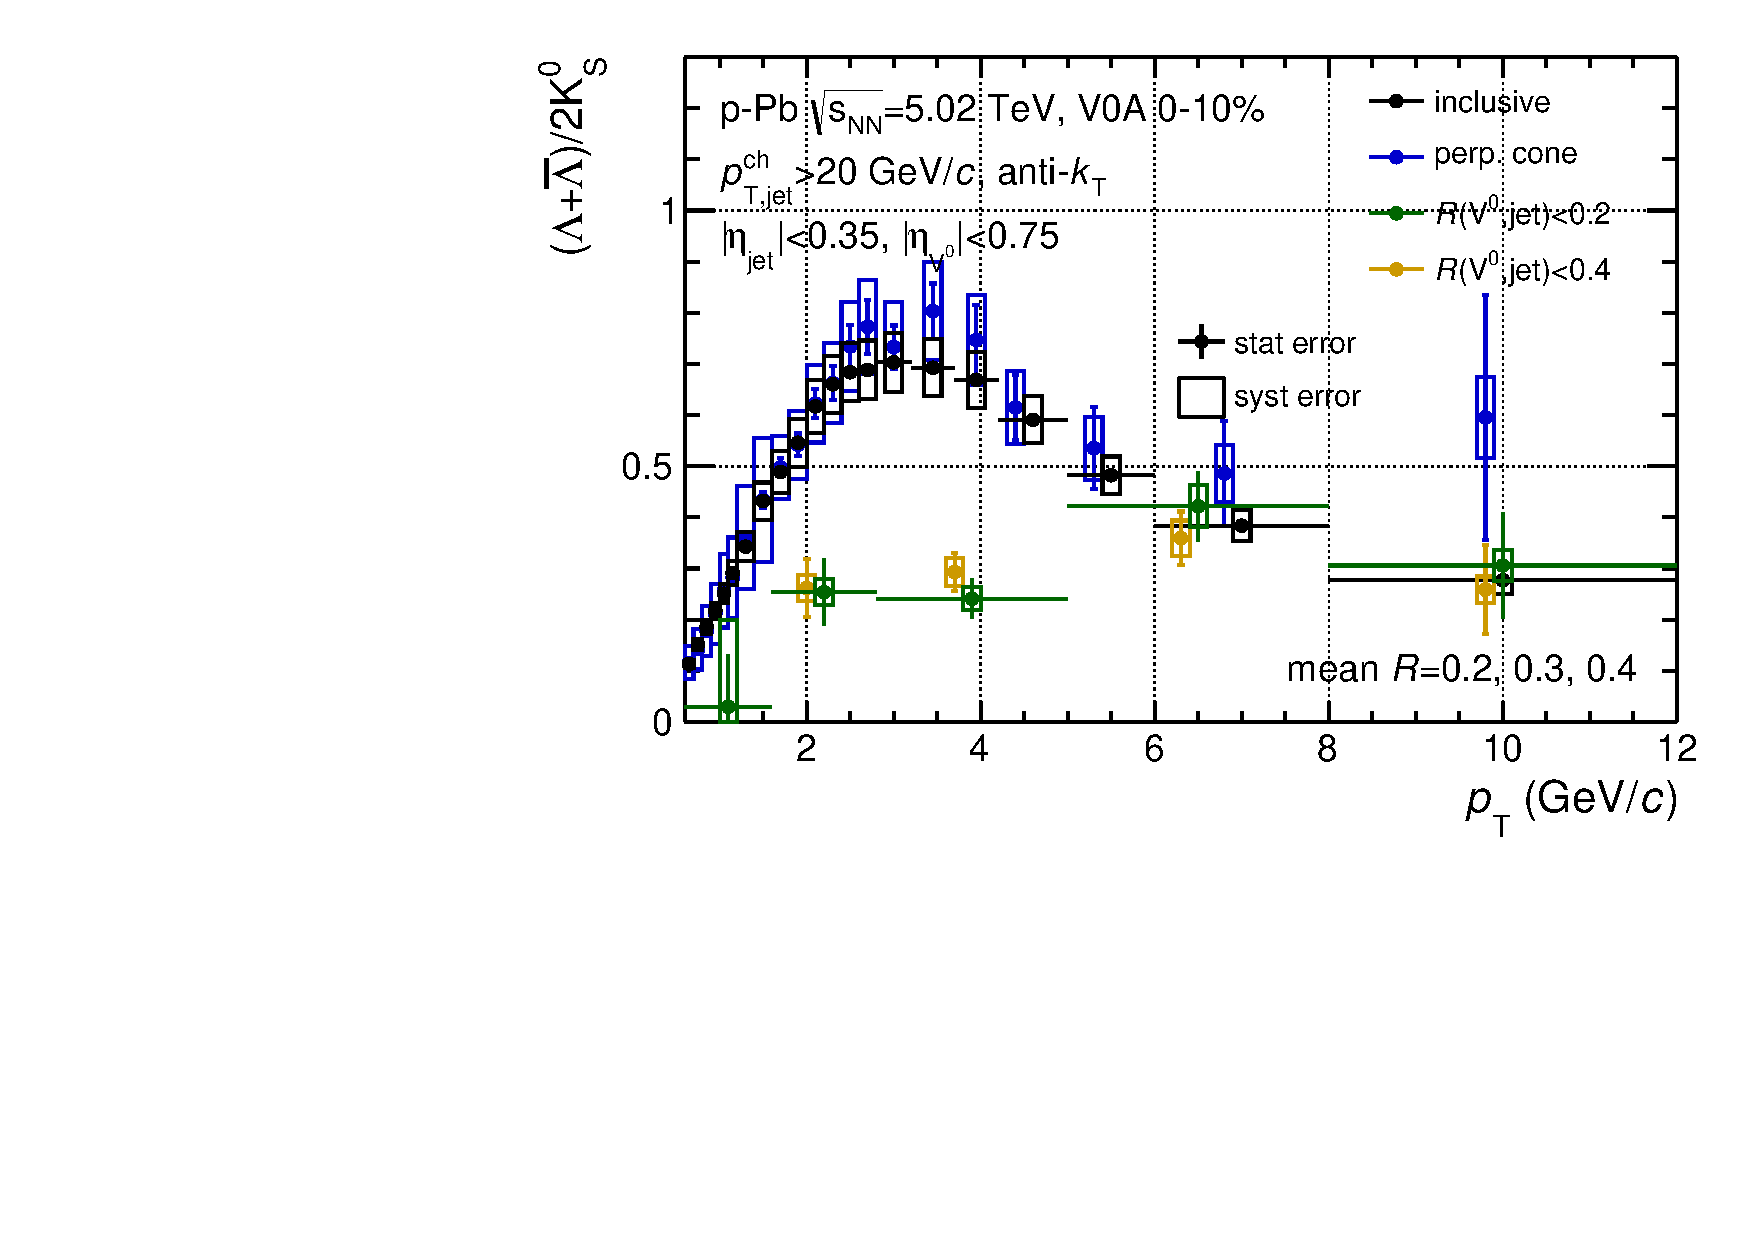
\includegraphics[width=.32\textwidth]{cL2K_Pt_Mean_V0A_000_010_PtJ20}
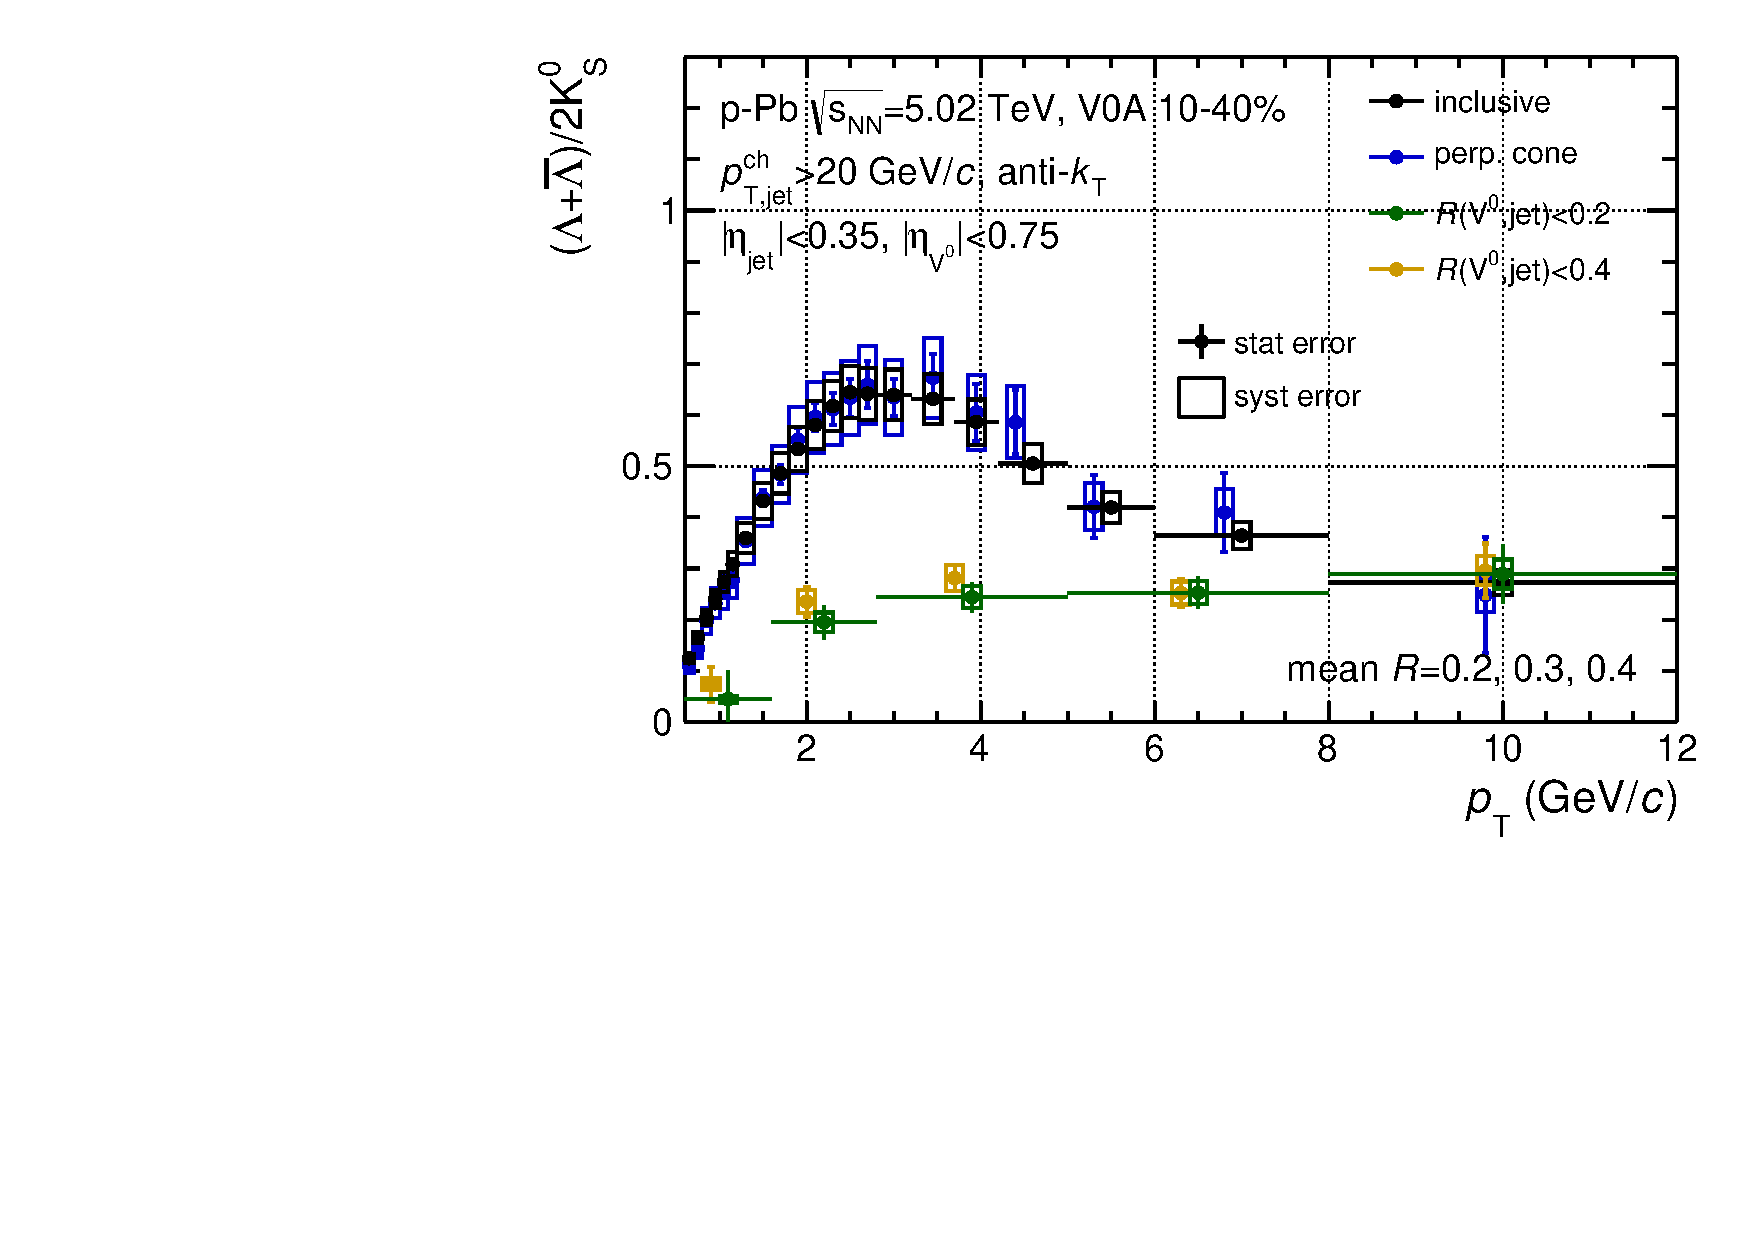
\includegraphics[width=.32\textwidth]{cL2K_Pt_Mean_V0A_010_040_PtJ20}
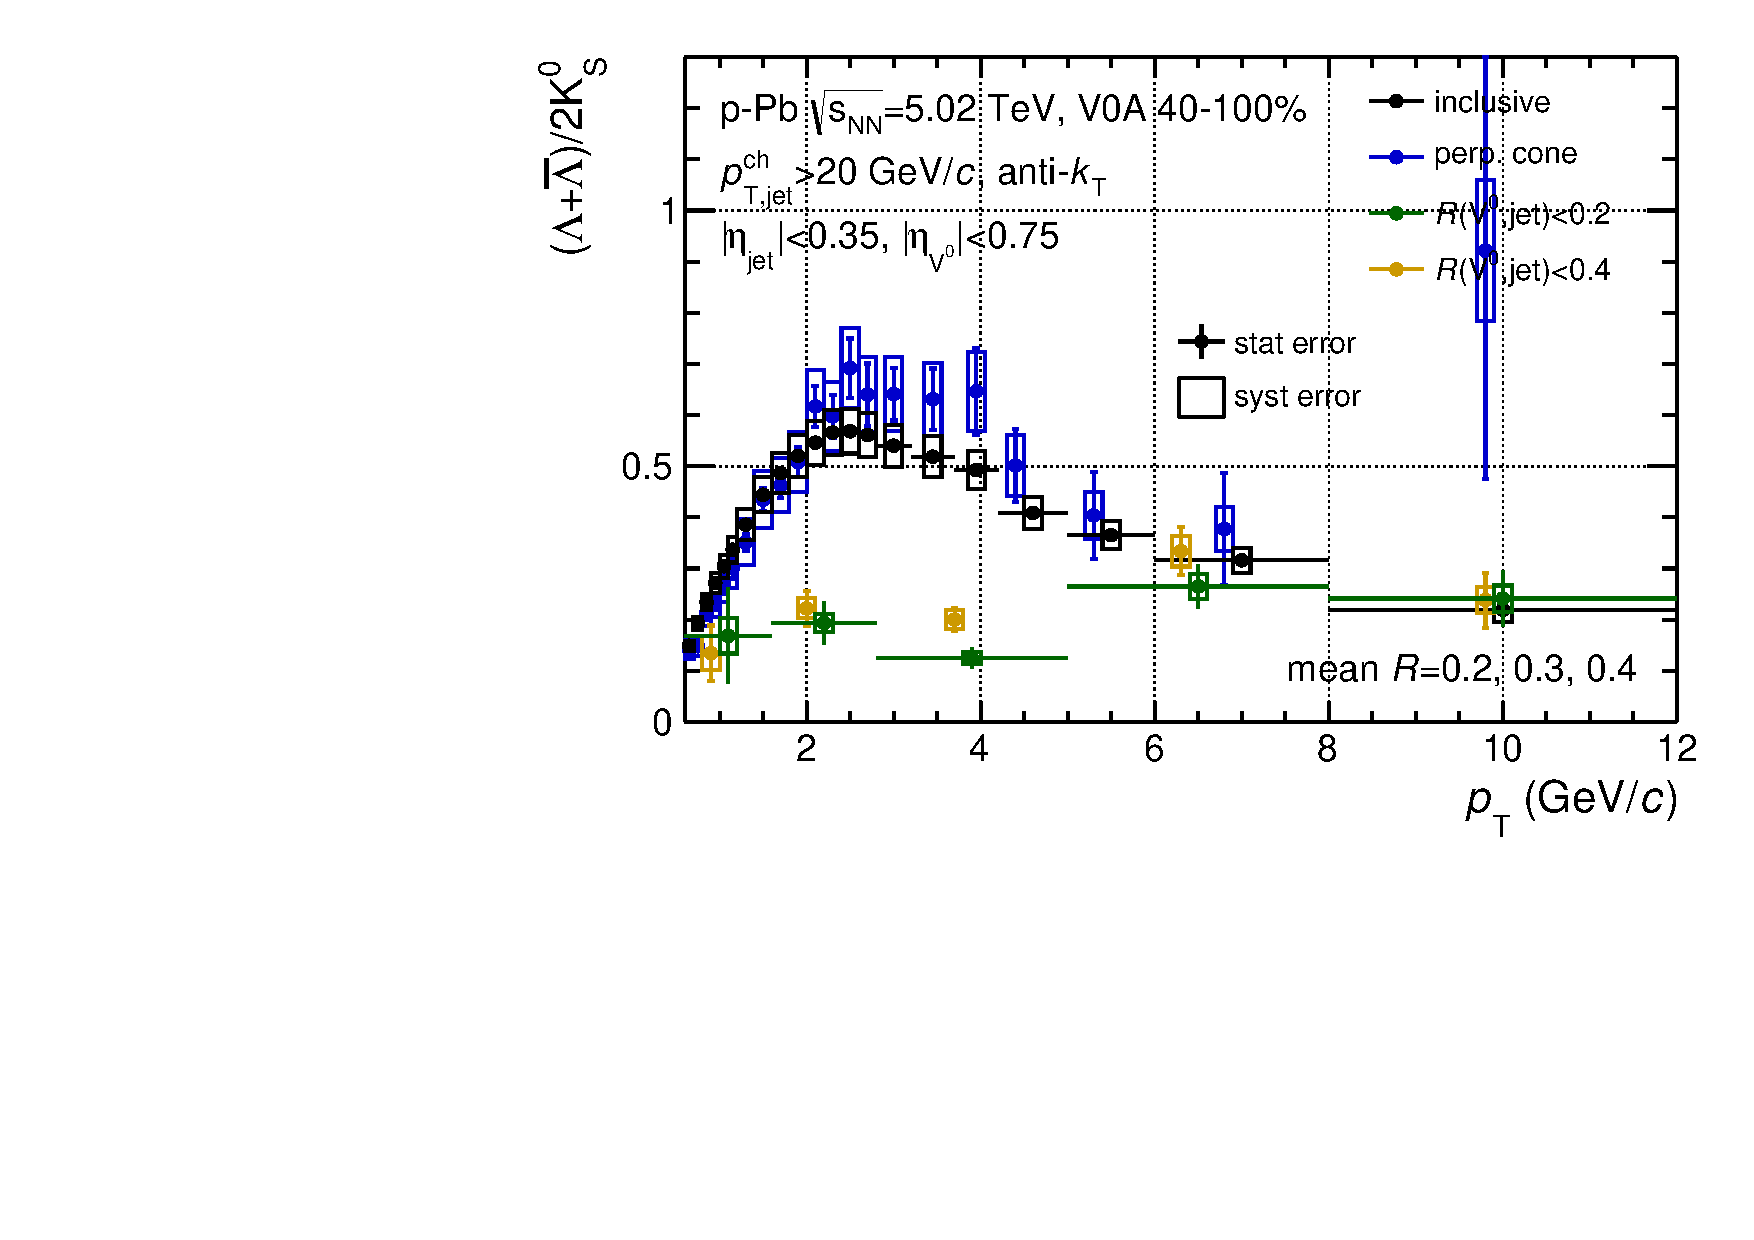
\includegraphics[width=.32\textwidth]{cL2K_Pt_Mean_V0A_040_100_PtJ20}
\caption{$\Lambda$-to-$\Kshort$ ratio as a function of $\pT$
  averaged over jets with
  $R=0.2,~0.3$ and $0.4$ in $p_{\rm T,jet}>20~\GeVc$.
  Two $\Vzero$--jet matching radii $R(\Vzero,{\rm jet})<0.2$ and $0.4$ are used.
  Results are shown in three V0A event activity classes and
  compared with the inclusive and the underlying $\Vzeros$.}
\label{fig:s01L2KJC0XV0APtj20}
\end{figure}


\begin{figure}[htbp]
\centering
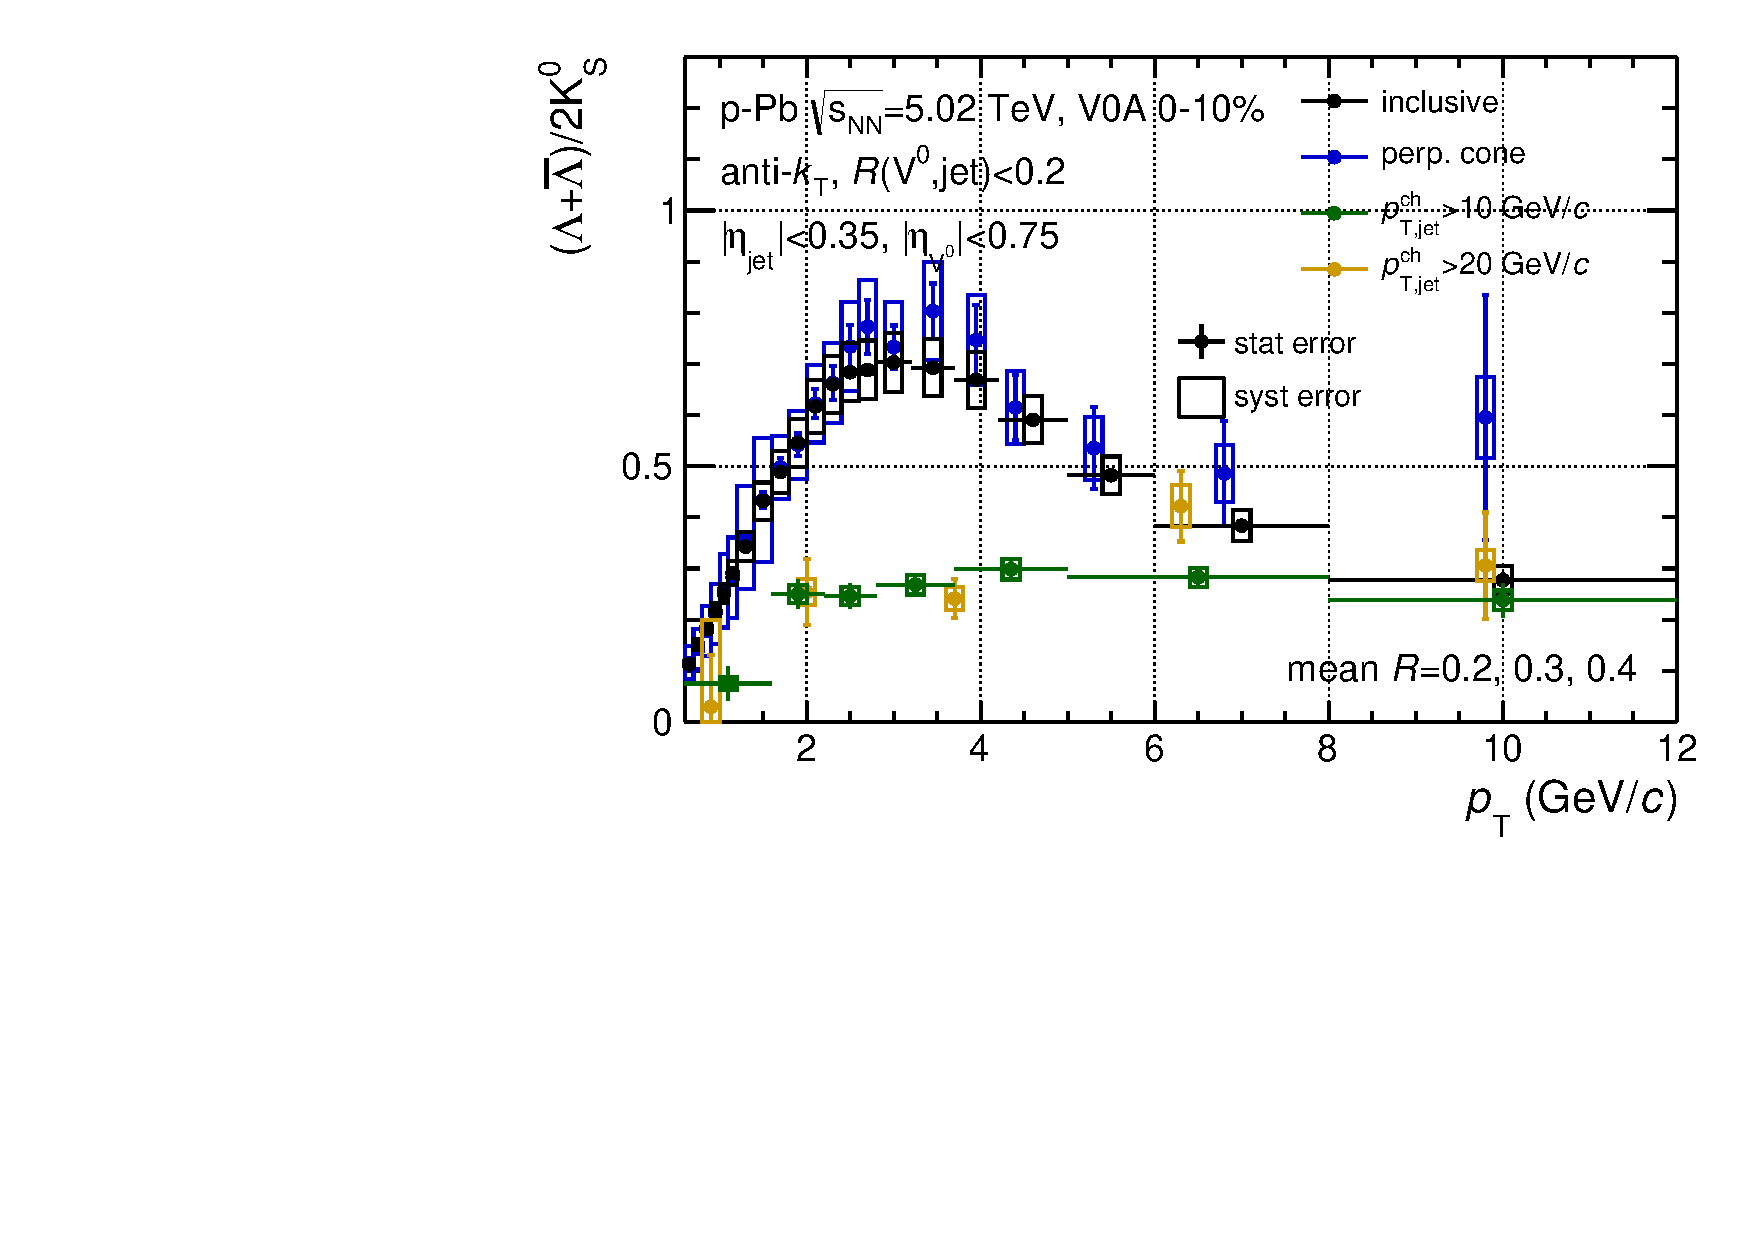
\includegraphics[width=.32\textwidth]{cL2K_Pt_PtJE_JC02_V0A_000_010}
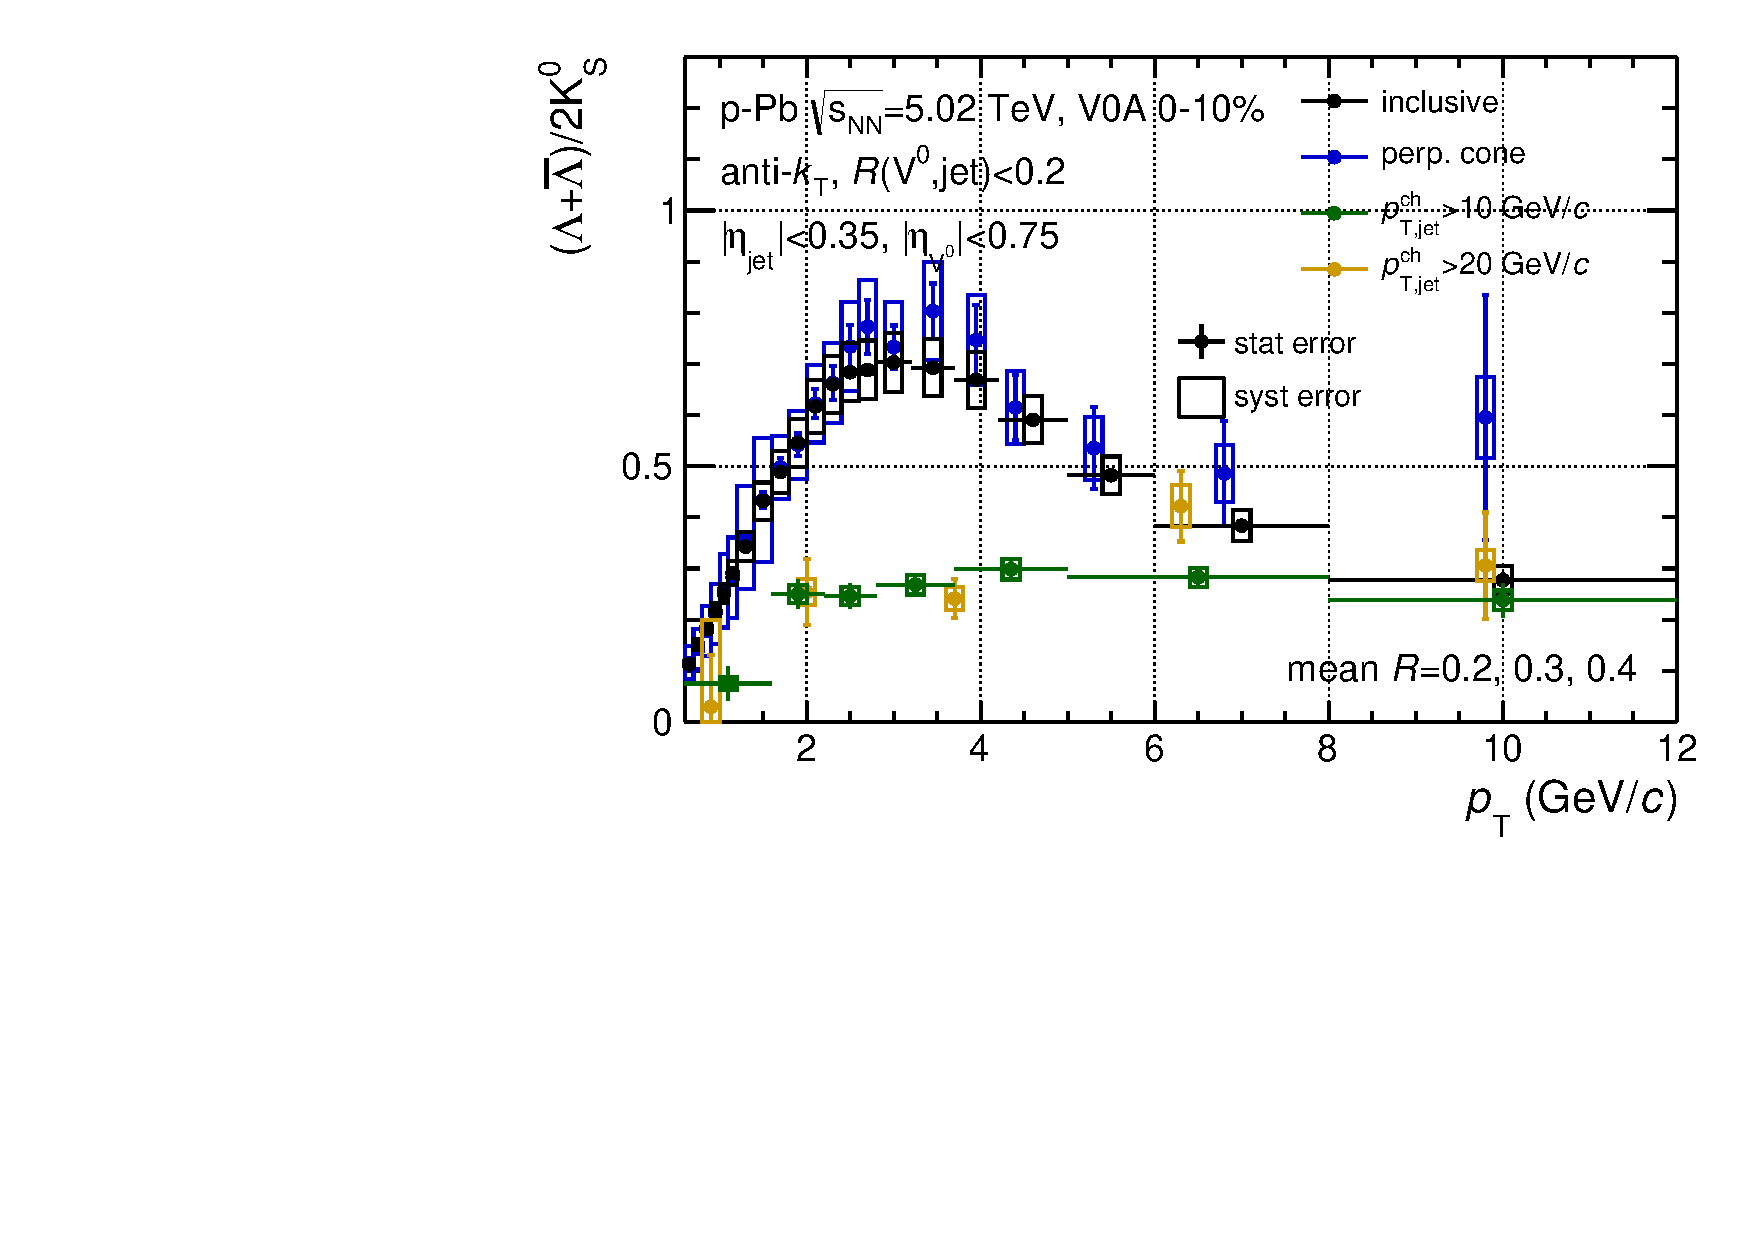
\includegraphics[width=.32\textwidth]{cL2K_Pt_PtJE_JC02_V0A_000_010}
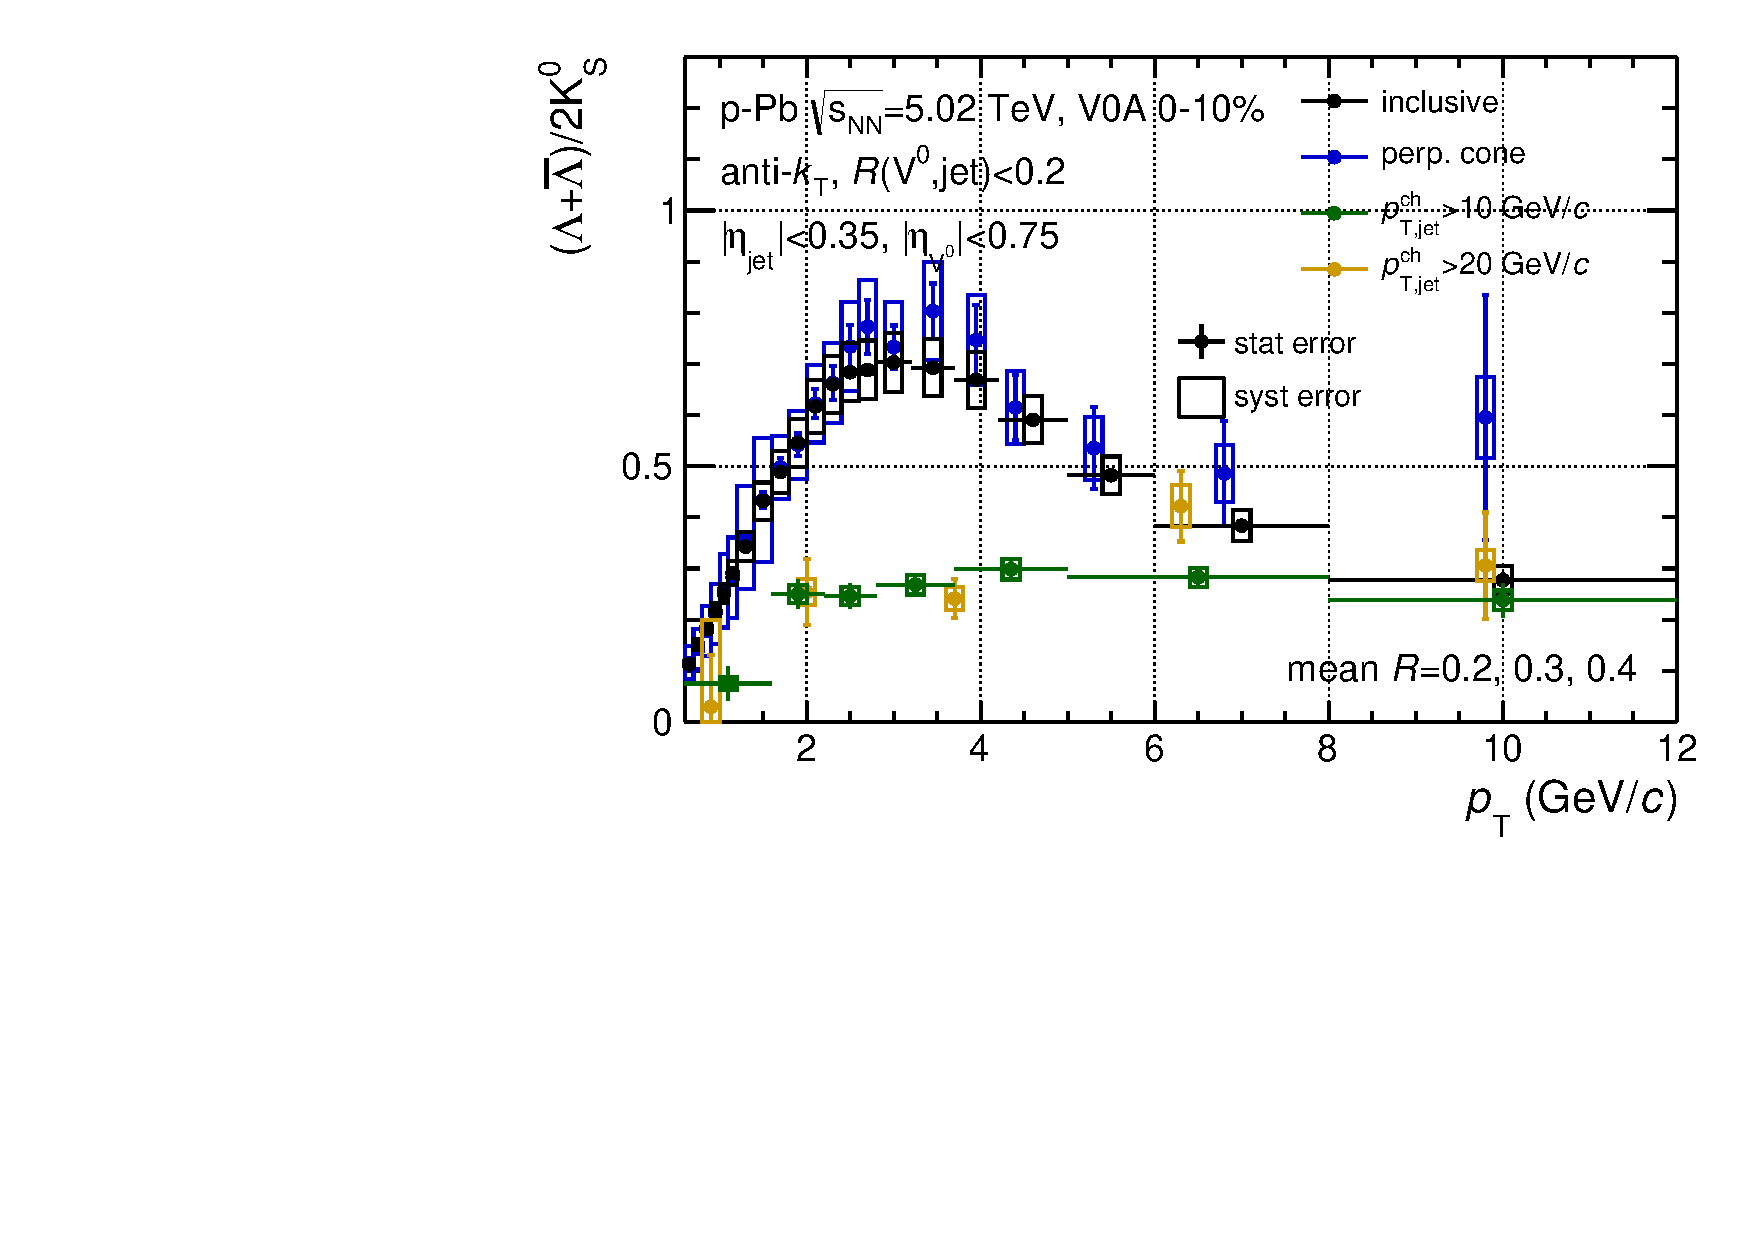
\includegraphics[width=.32\textwidth]{cL2K_Pt_PtJE_JC02_V0A_000_010}
\caption{$\Lambda$-to-$\Kshort$ ratio as a function of $\pT$
  averaged over jets with
  $R=0.2,~0.3$ and $0.4$ in $p_{\rm T,jet}>10$ and $>20~\GeVc$,
  respectively.
  $\Vzero$--jet matching radius $R(\Vzero,{\rm jet})<0.2$.
  Results are shown in three V0A event activity classes and
  compared with the inclusive and the underlying $\Vzeros$.}
\label{fig:s01L2KJC02V0APtjXX}
\end{figure}

\begin{figure}[htbp]
\centering
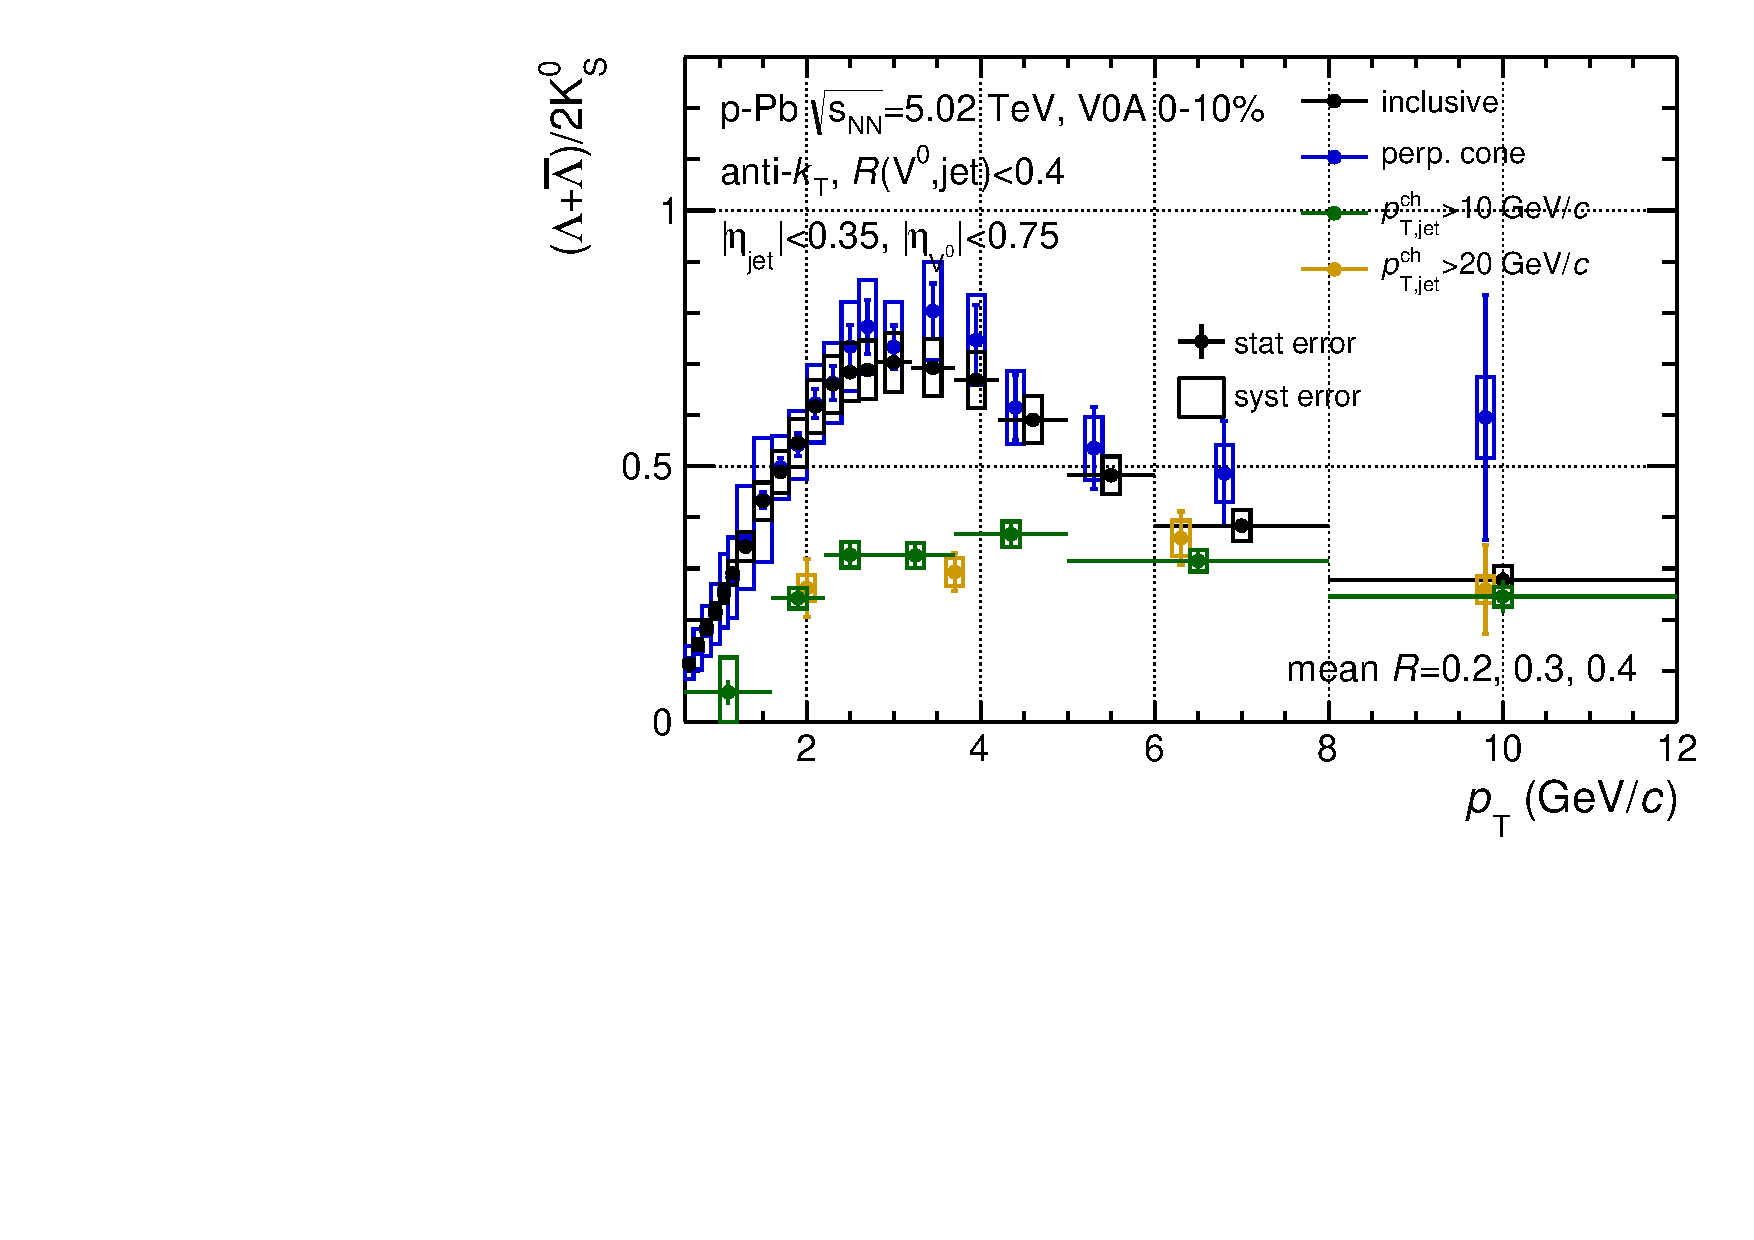
\includegraphics[width=.32\textwidth]{cL2K_Pt_PtJE_JC04_V0A_000_010}
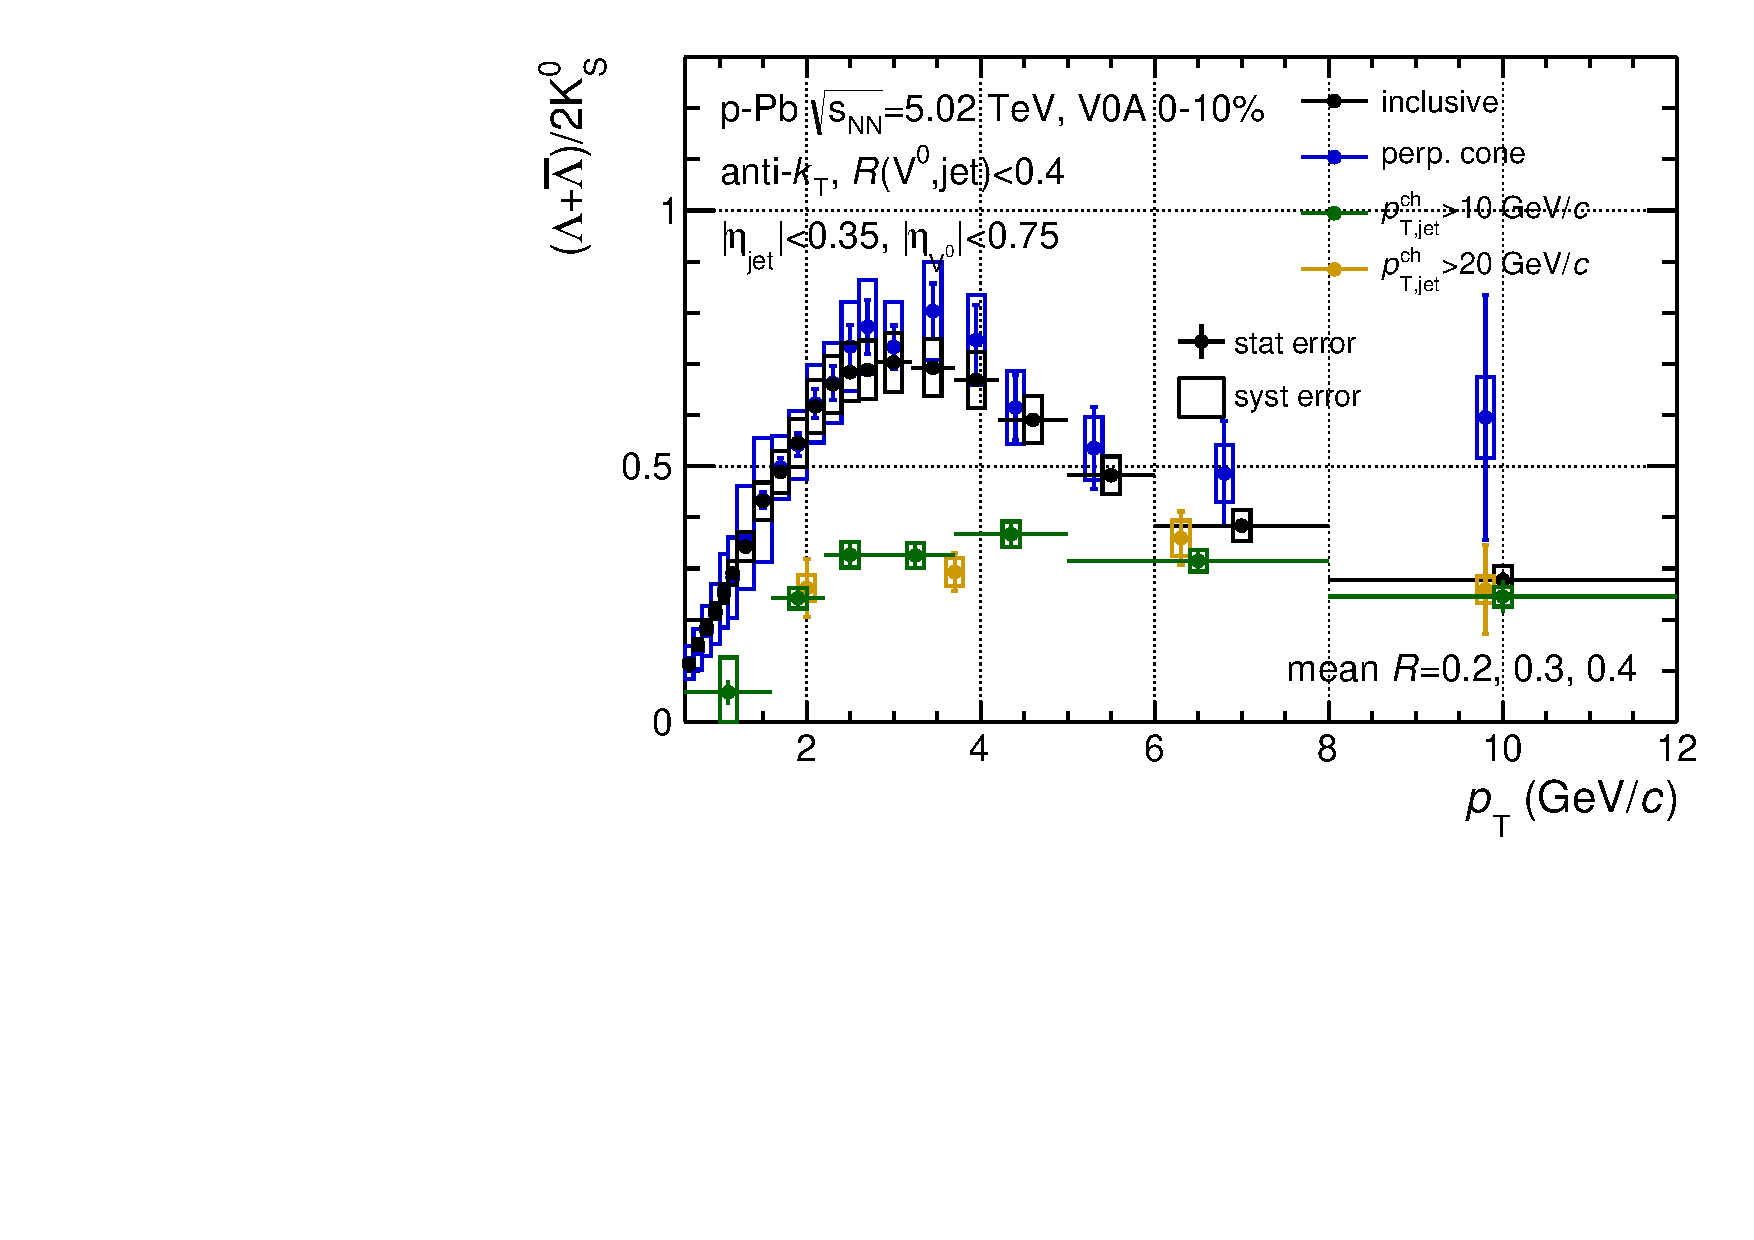
\includegraphics[width=.32\textwidth]{cL2K_Pt_PtJE_JC04_V0A_000_010}
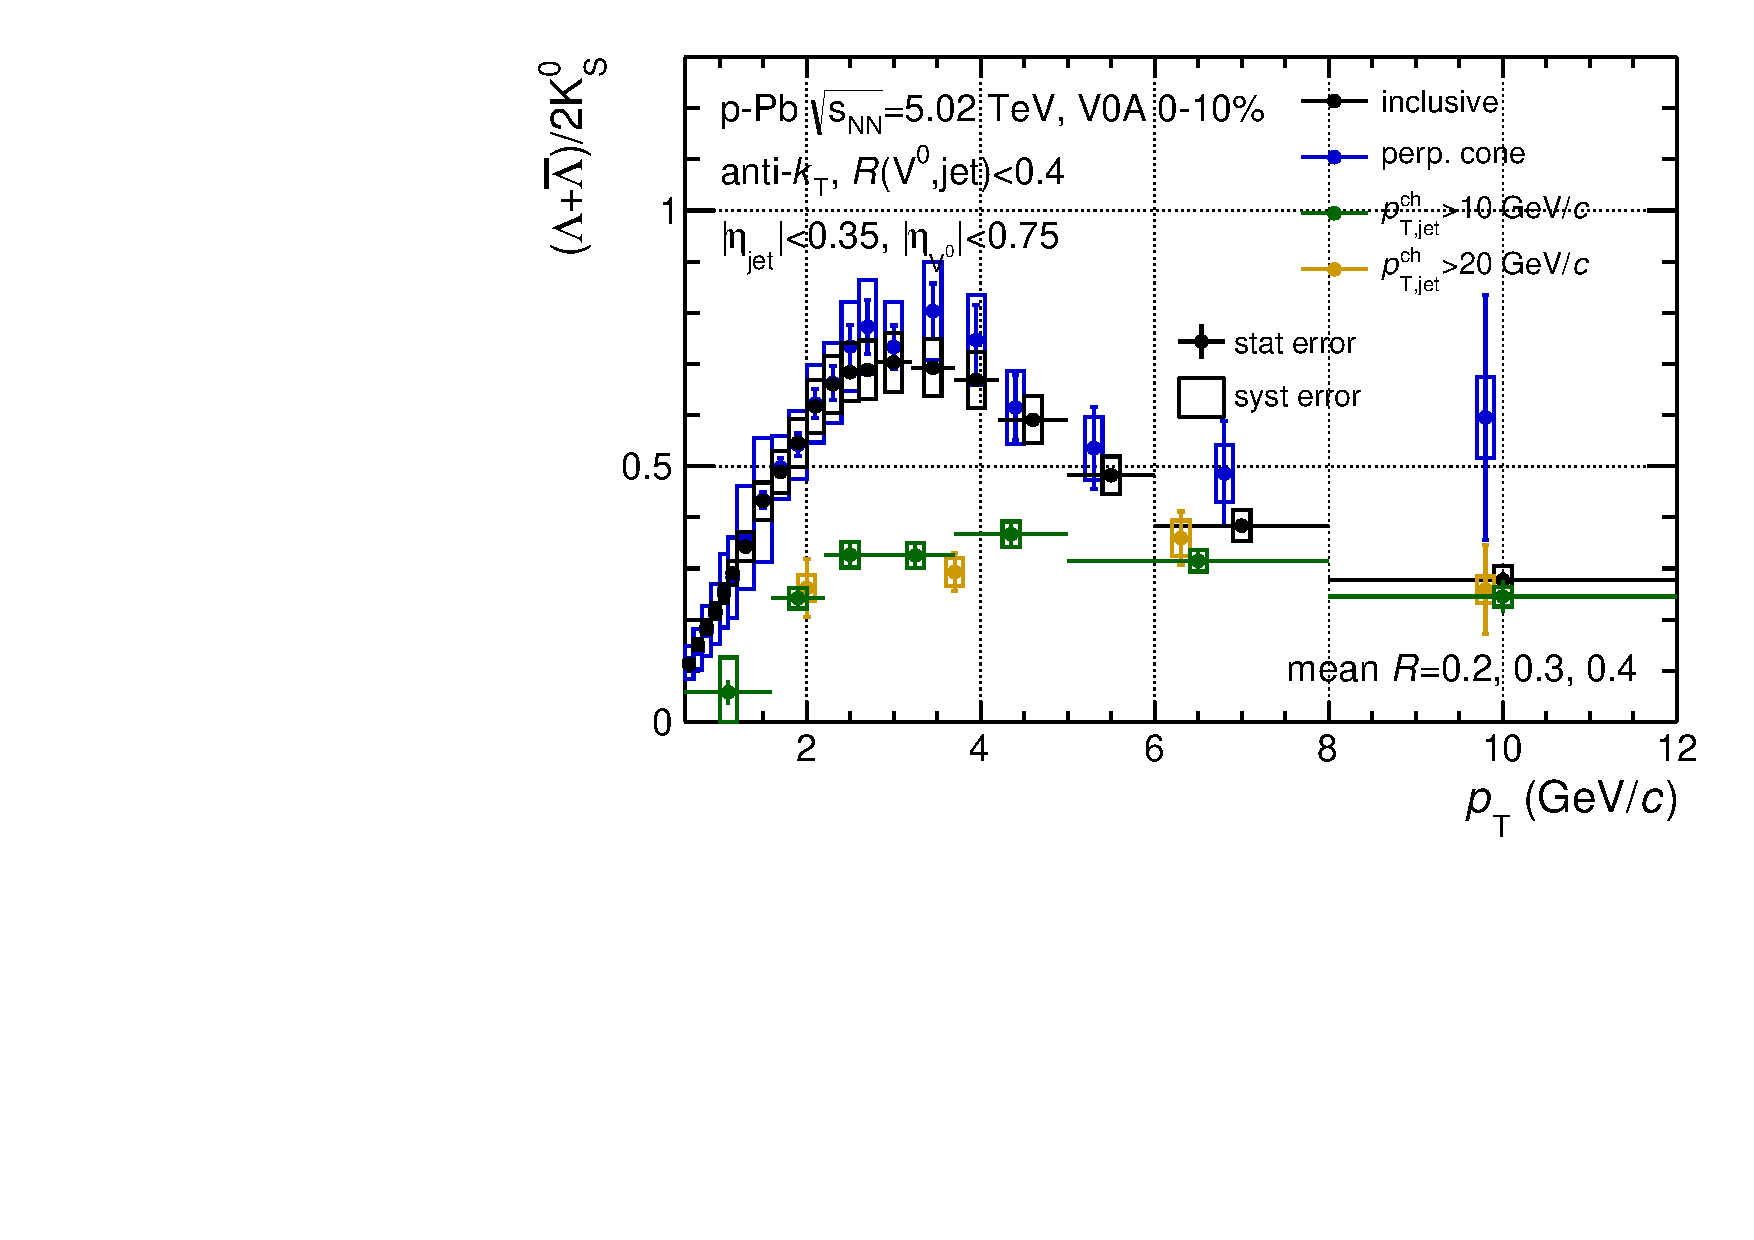
\includegraphics[width=.32\textwidth]{cL2K_Pt_PtJE_JC04_V0A_000_010}
\caption{$\Lambda$-to-$\Kshort$ ratio as a function of $\pT$
  averaged over jets with
  $R=0.2,~0.3$ and $0.4$ in $p_{\rm T,jet}>10$ and $>20~\GeVc$,
  respectively.
  $\Vzero$--jet matching radius $R(\Vzero,{\rm jet})<0.4$.
  Results are shown in three V0A event activity classes and
  compared with the inclusive and the underlying $\Vzeros$.}
\label{fig:s01L2KJC04V0APtjXX}
\end{figure}
%%%%%%%%%%%%%%%%%%%%%%%%%%%%%%%%%%%%%%%%%%%%%%%%%%%%%%%%%%%%%%%%%%%%%%%%%%%%%%%

\newpage
\subsubsection{ZNA Event Activity Estimator}

\begin{figure}[htbp]
\centering
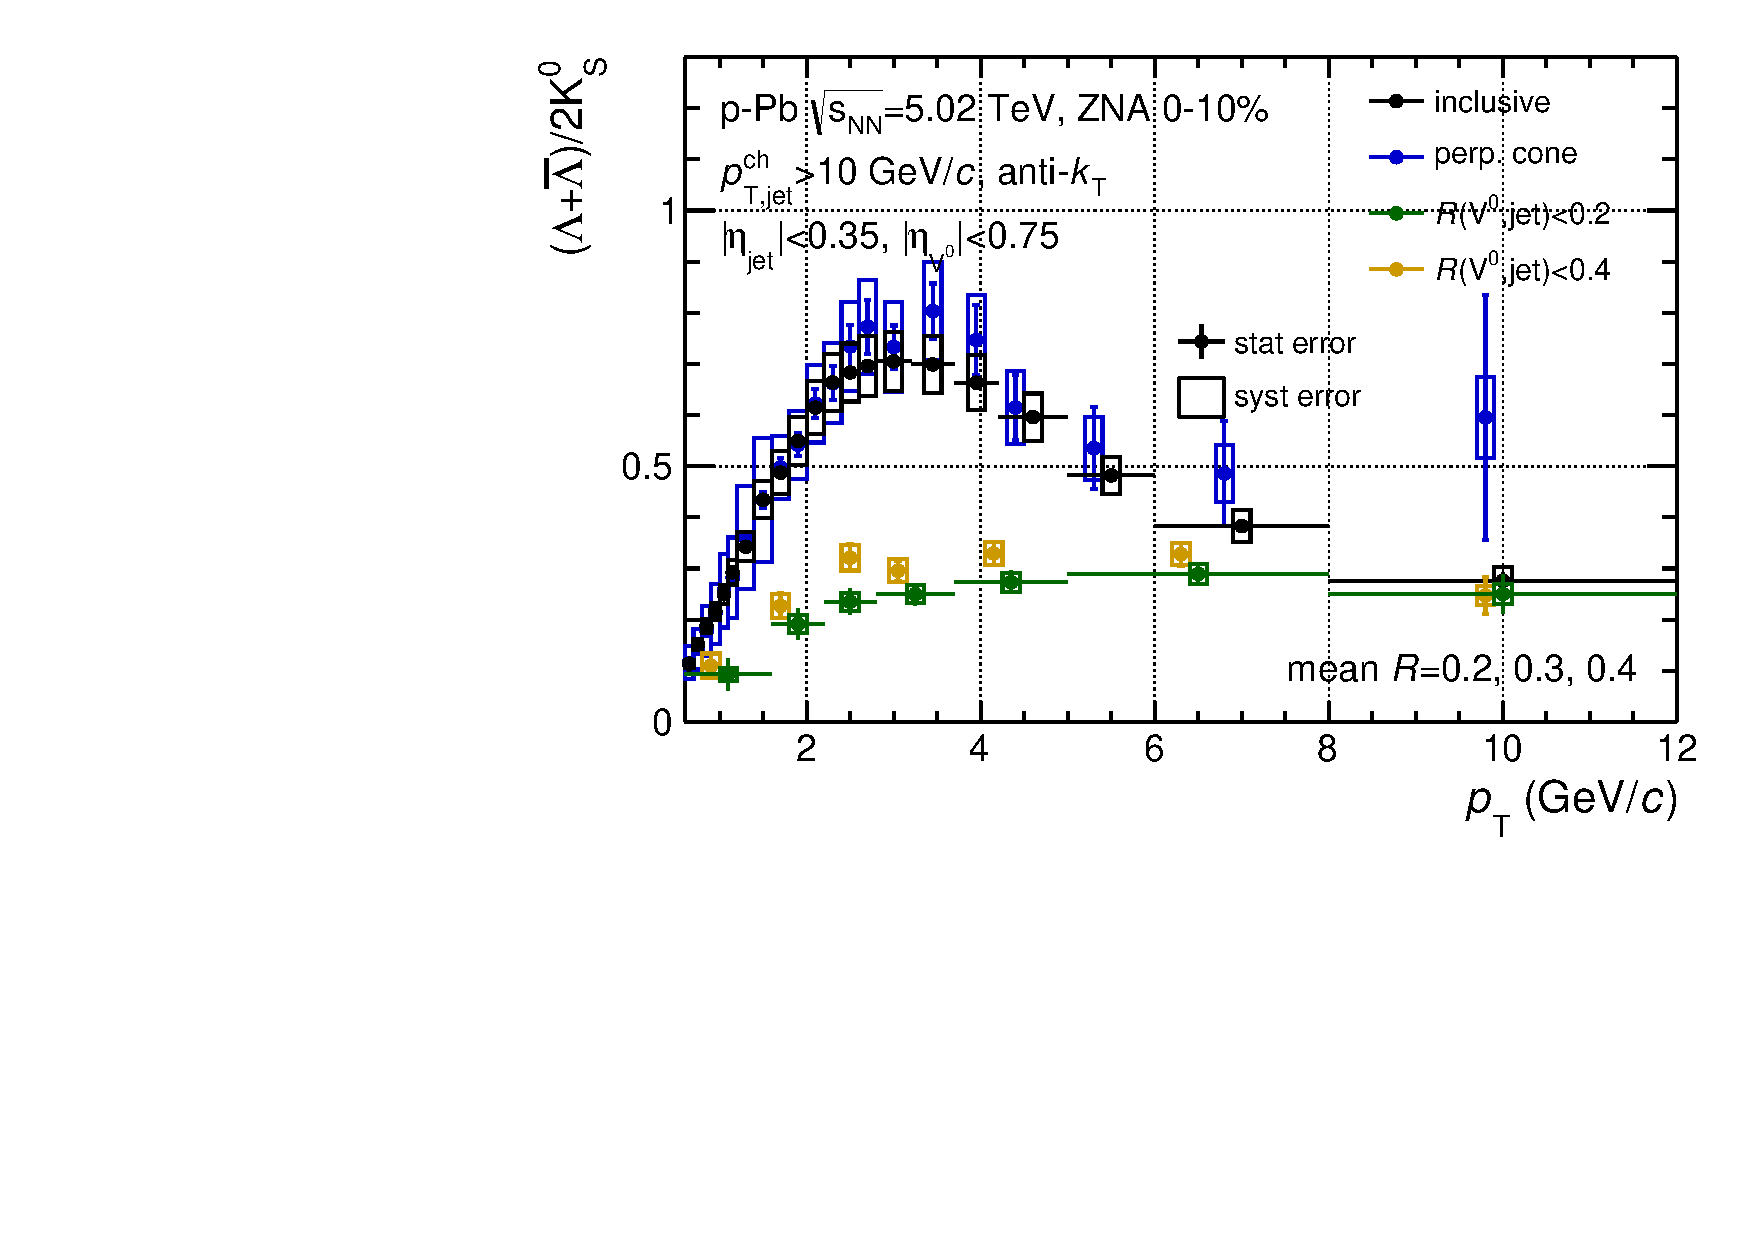
\includegraphics[width=.32\textwidth]{cL2K_Pt_Mean_ZNA_000_010_PtJ10}
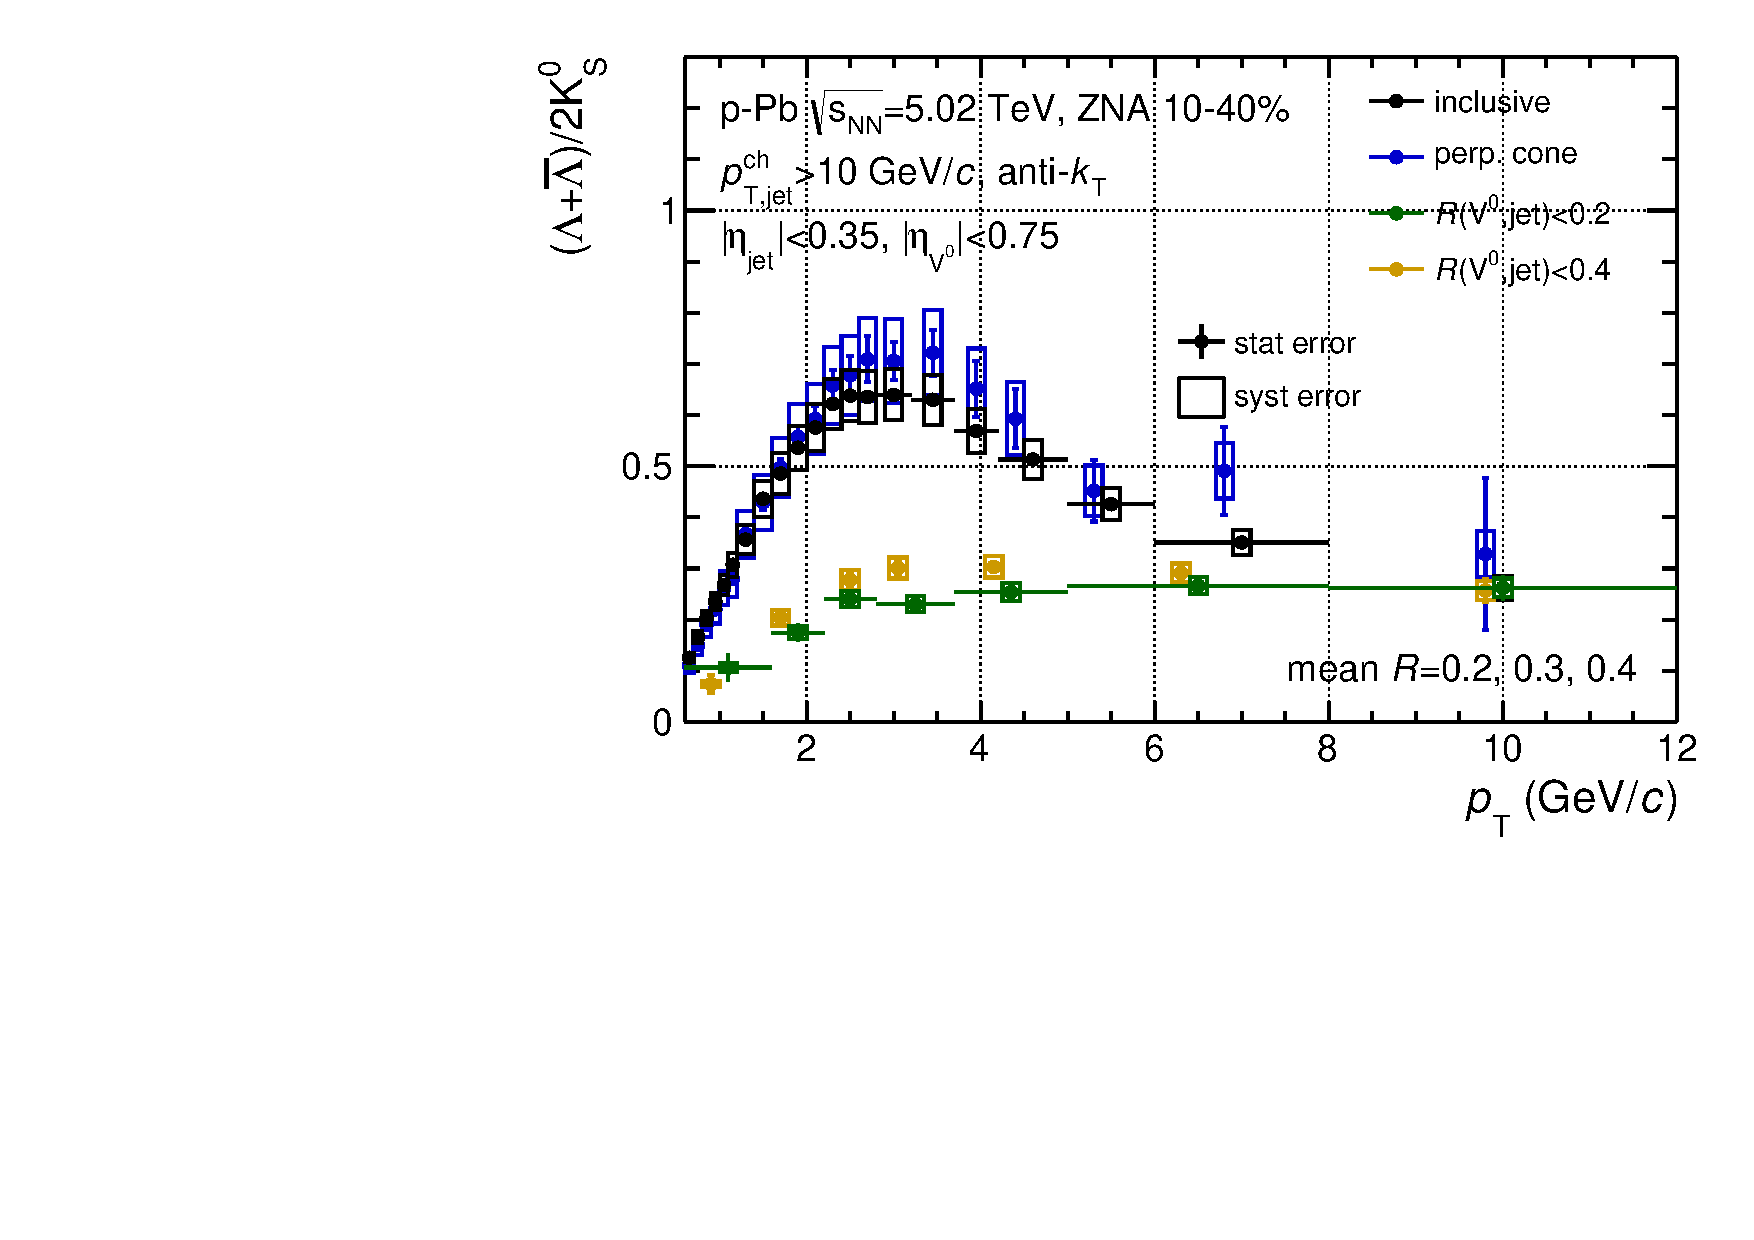
\includegraphics[width=.32\textwidth]{cL2K_Pt_Mean_ZNA_010_040_PtJ10}
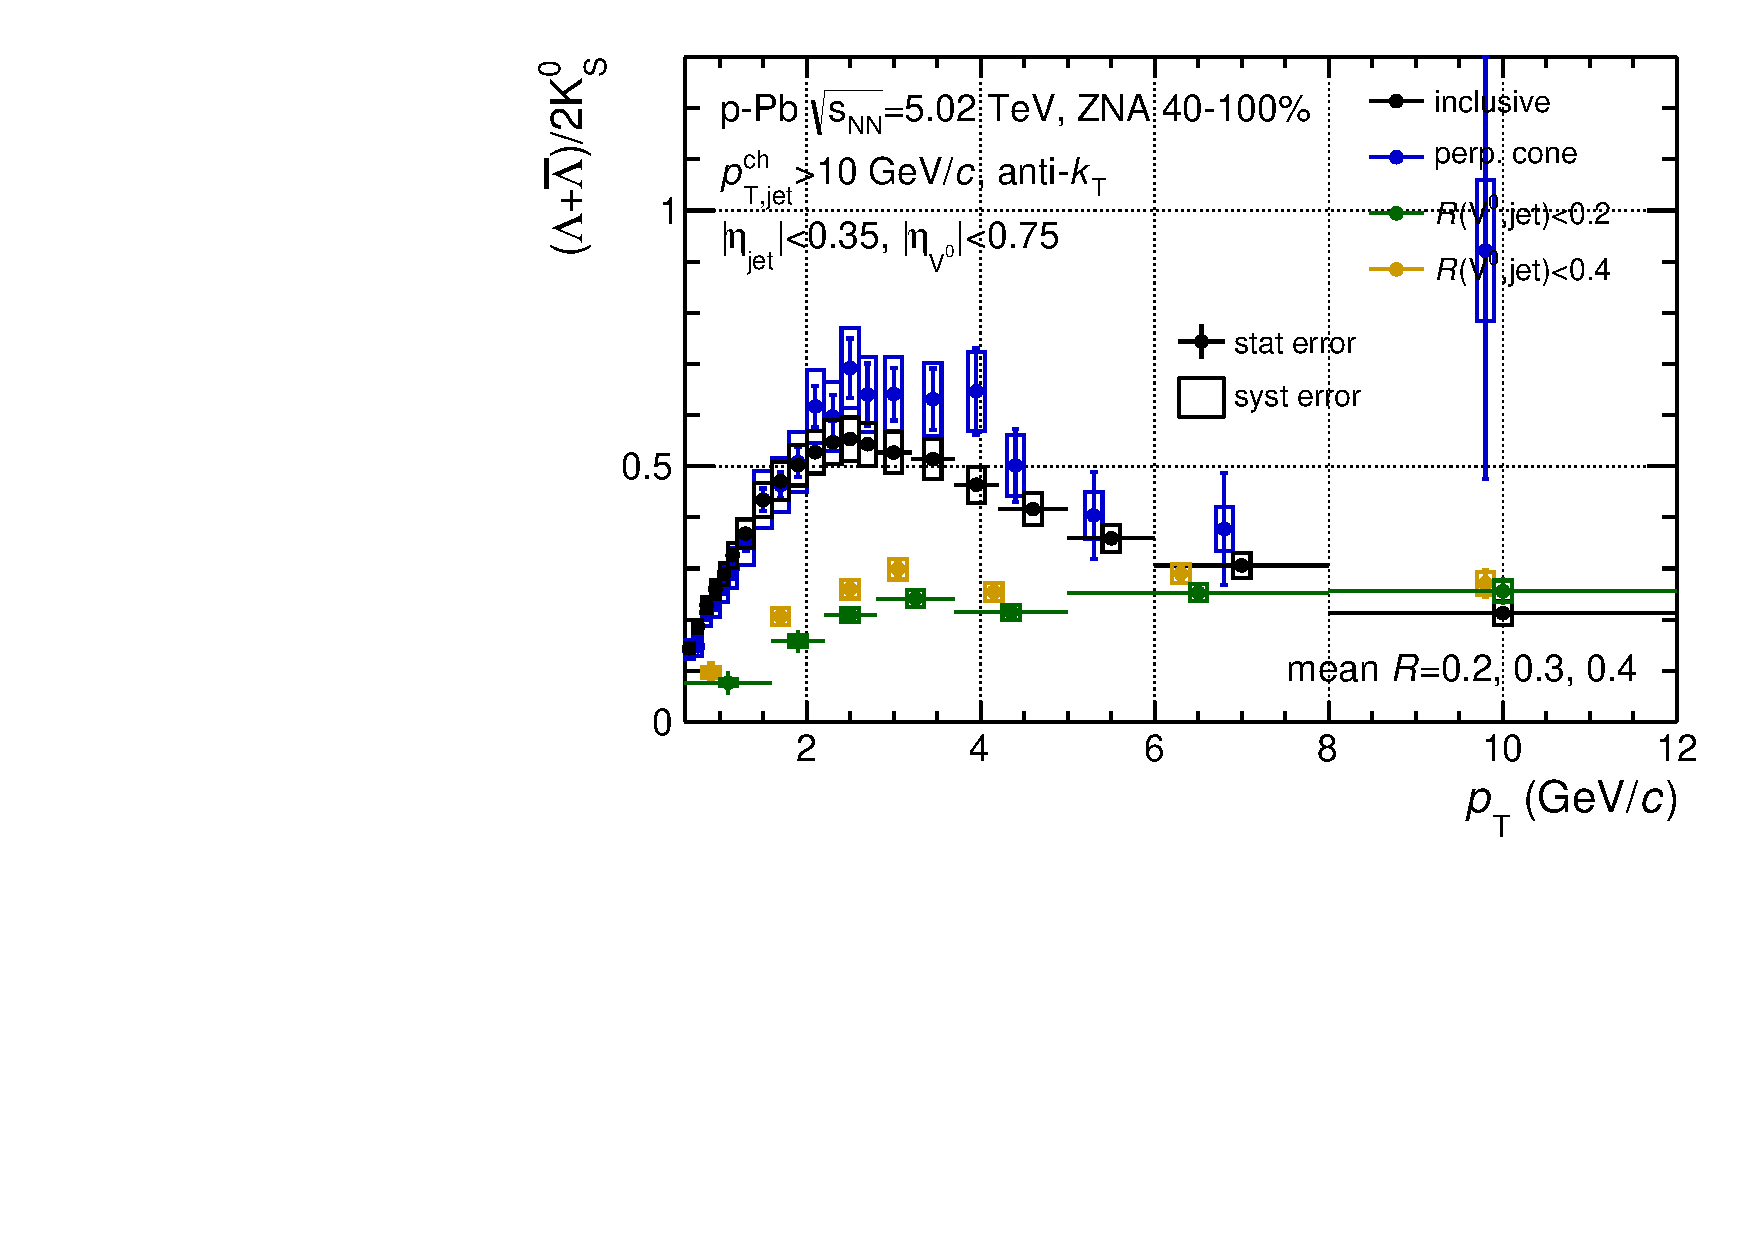
\includegraphics[width=.32\textwidth]{cL2K_Pt_Mean_ZNA_040_100_PtJ10}
\caption{$\Lambda$-to-$\Kshort$ ratio as a function of $\pT$
  averaged over jets with
  $R=0.2,~0.3$ and $0.4$ in $p_{\rm T,jet}>10~\GeVc$.
  Two $\Vzero$--jet matching radii $R(\Vzero,{\rm jet})<0.2$ and $0.4$ are used.
  Results are shown in three ZNA event activity classes and
  compared with the inclusive and the underlying $\Vzeros$.}
\label{fig:s01L2KJC0XZNAPtj10}
\end{figure}

\begin{figure}[htbp]
\centering
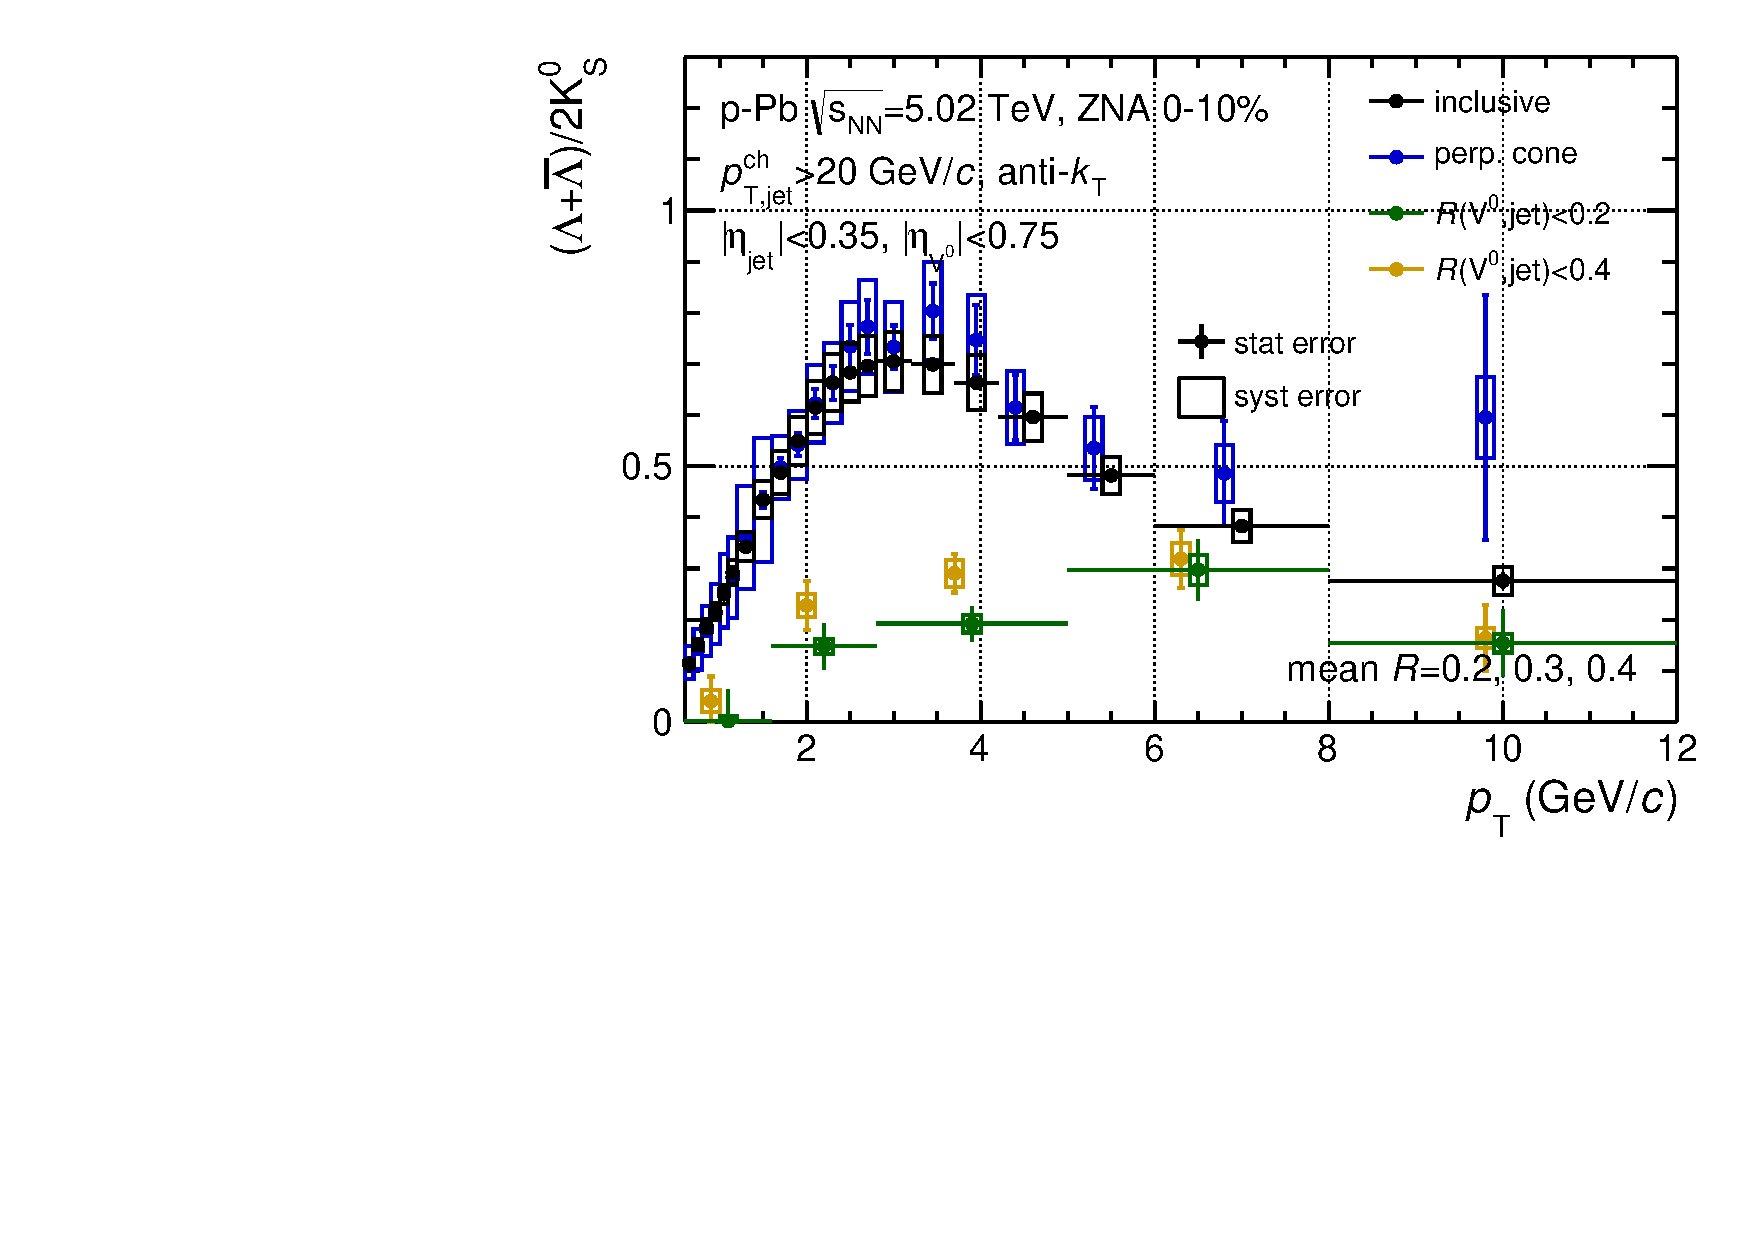
\includegraphics[width=.32\textwidth]{cL2K_Pt_Mean_ZNA_000_010_PtJ20}
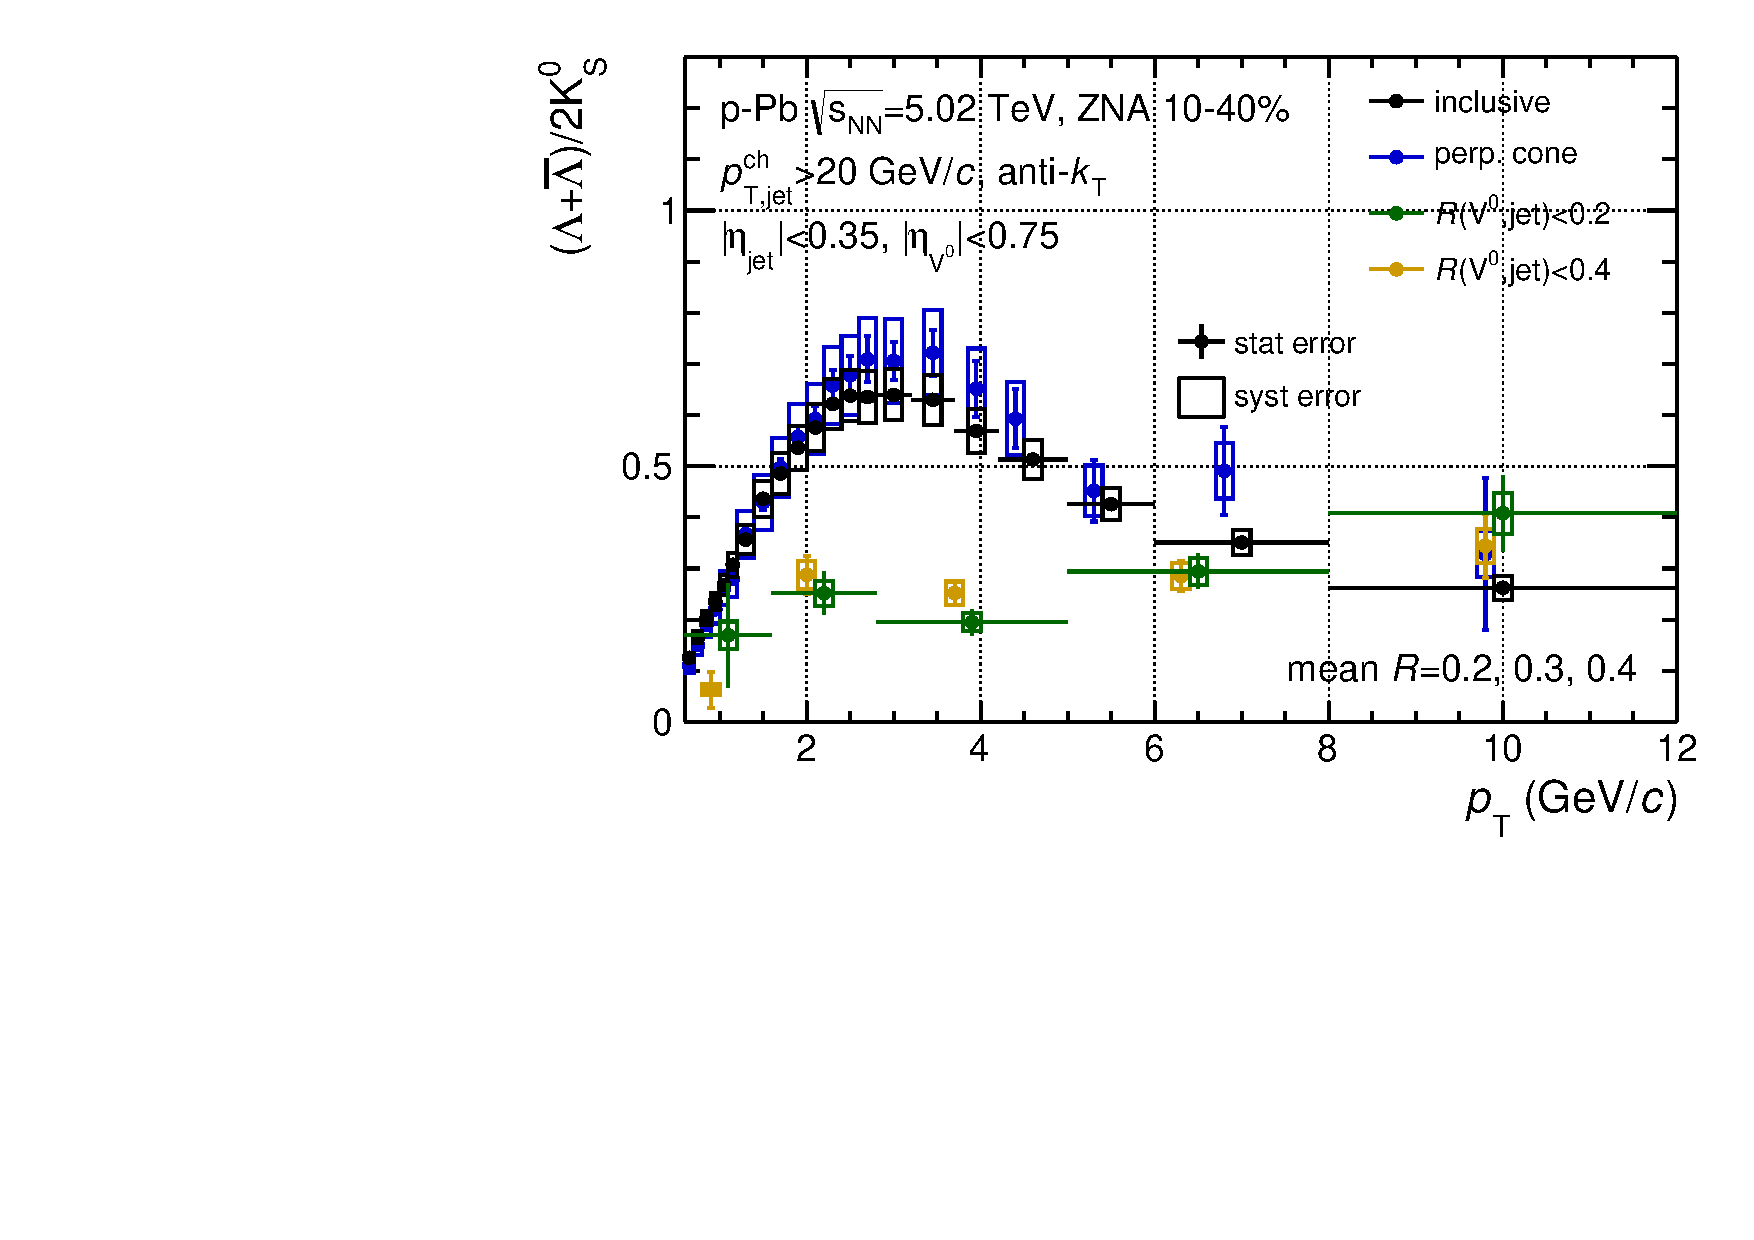
\includegraphics[width=.32\textwidth]{cL2K_Pt_Mean_ZNA_010_040_PtJ20}
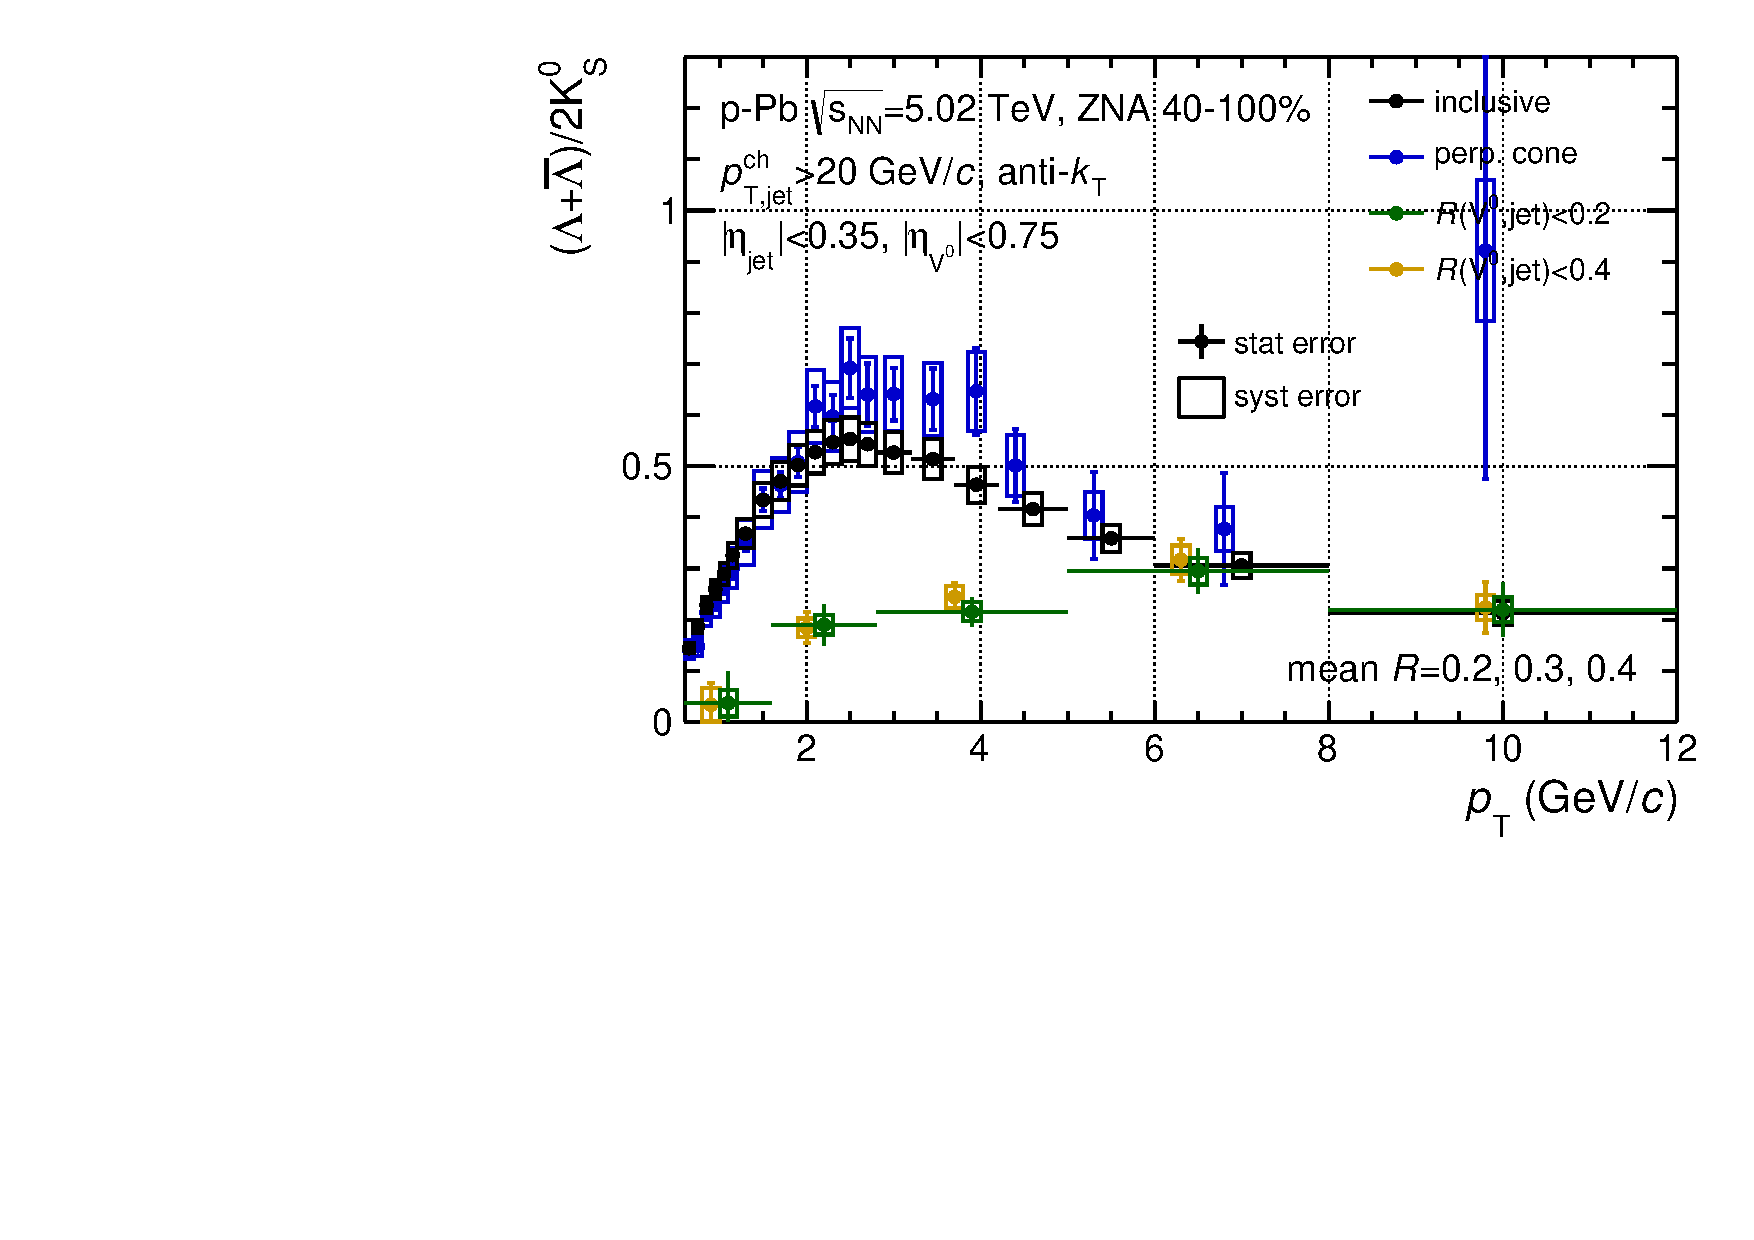
\includegraphics[width=.32\textwidth]{cL2K_Pt_Mean_ZNA_040_100_PtJ20}
\caption{$\Lambda$-to-$\Kshort$ ratio as a function of $\pT$
  averaged over jets with
  $R=0.2,~0.3$ and $0.4$ in $p_{\rm T,jet}>20~\GeVc$.
  Two $\Vzero$--jet matching radii $R(\Vzero,{\rm jet})<0.2$ and $0.4$ are used.
  Results are shown in three ZNA event activity classes and
  compared with the inclusive and the underlying $\Vzeros$.}
\label{fig:s01L2KJC0XZNAPtj20}
\end{figure}

\begin{figure}[htbp]
\centering
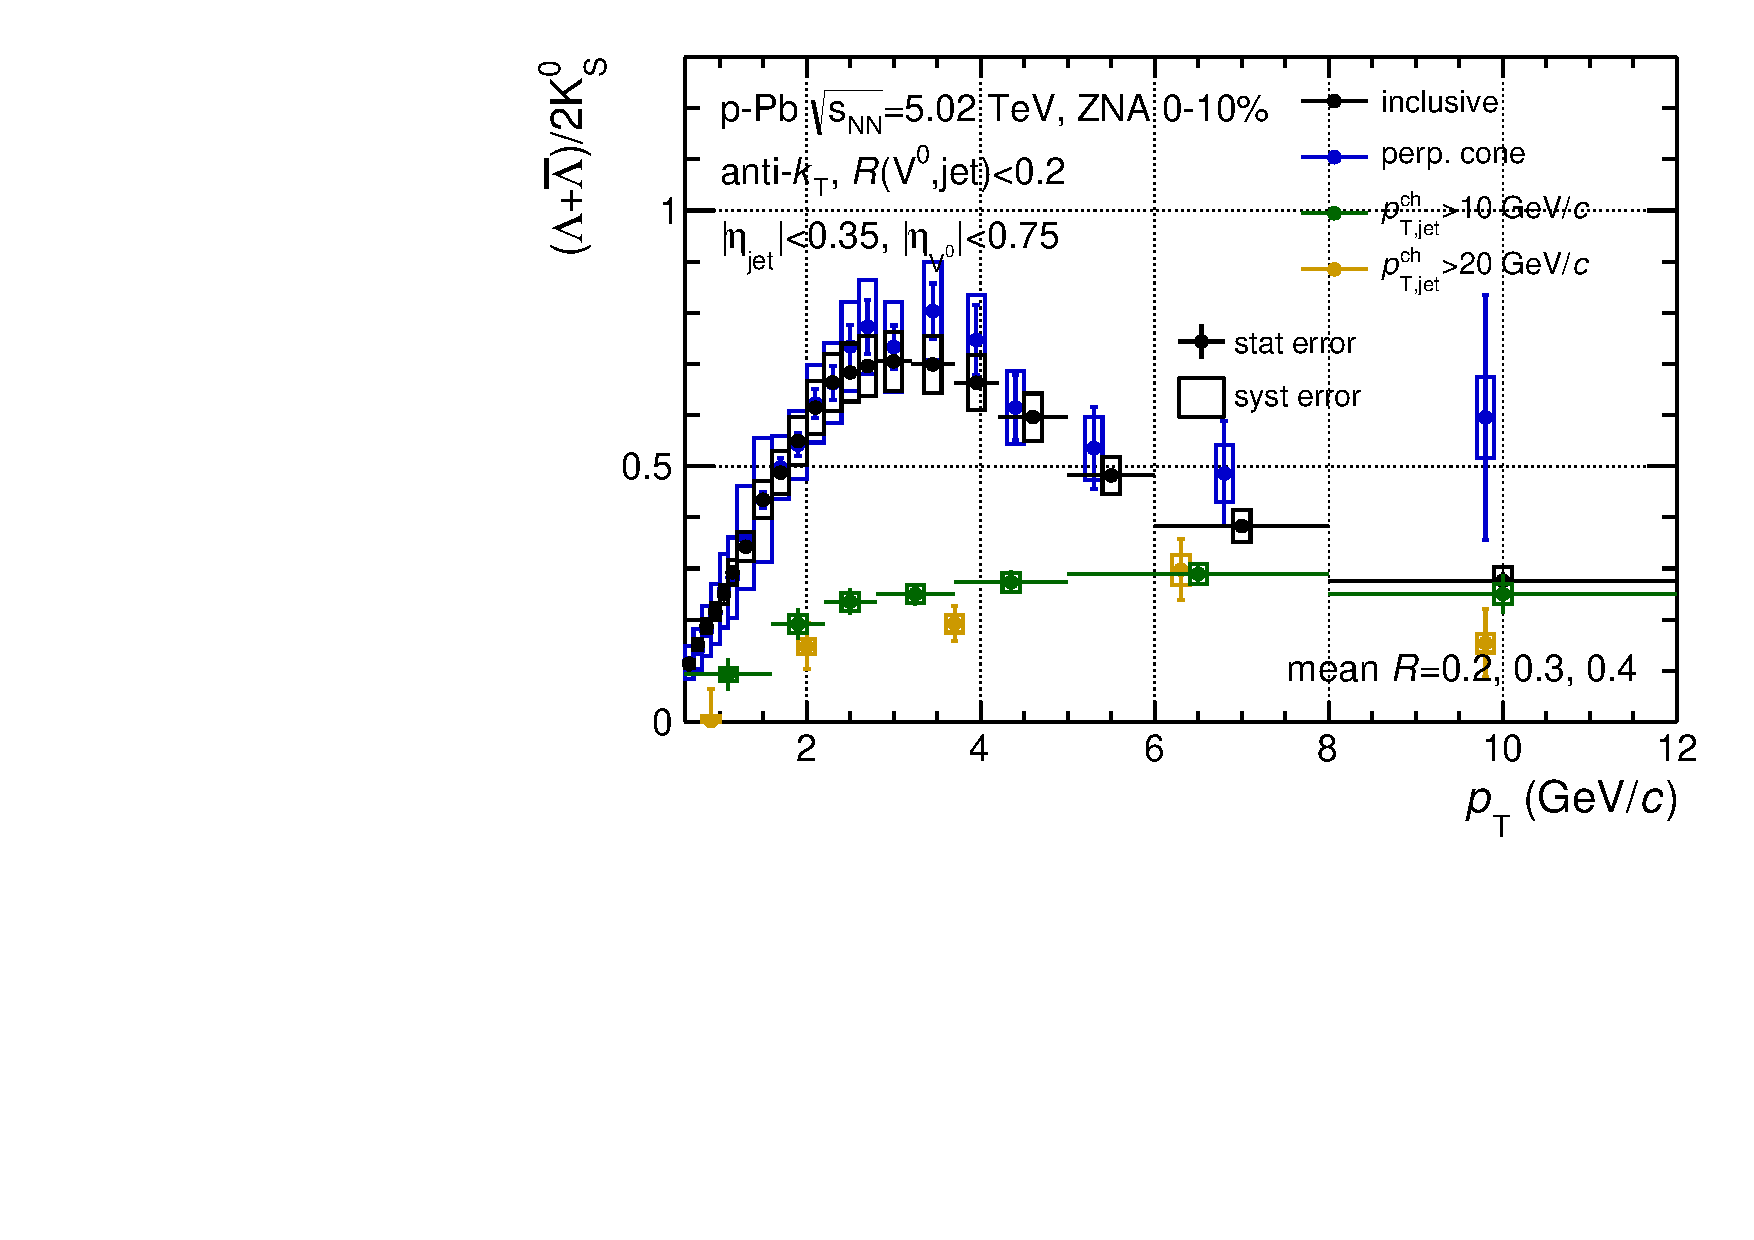
\includegraphics[width=.32\textwidth]{cL2K_Pt_PtJE_JC02_ZNA_000_010}
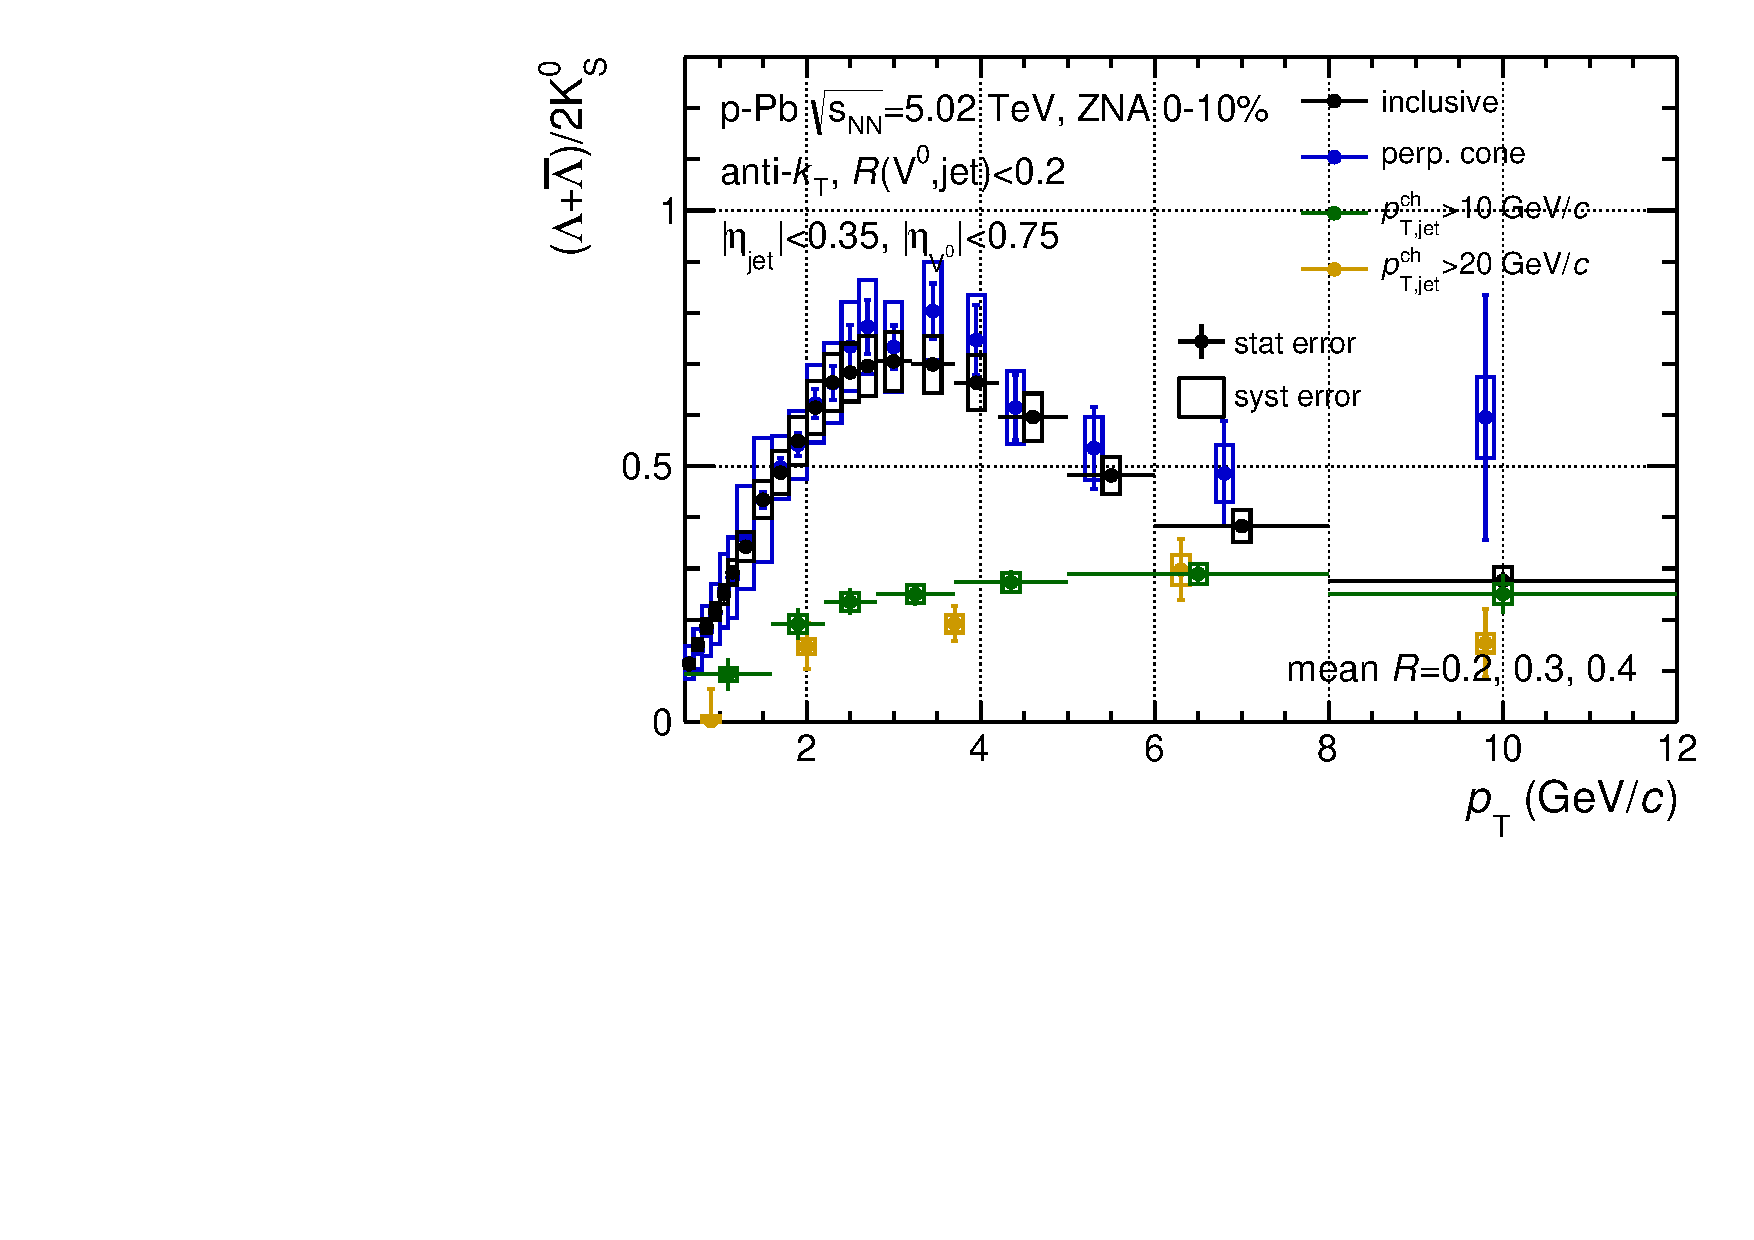
\includegraphics[width=.32\textwidth]{cL2K_Pt_PtJE_JC02_ZNA_000_010}
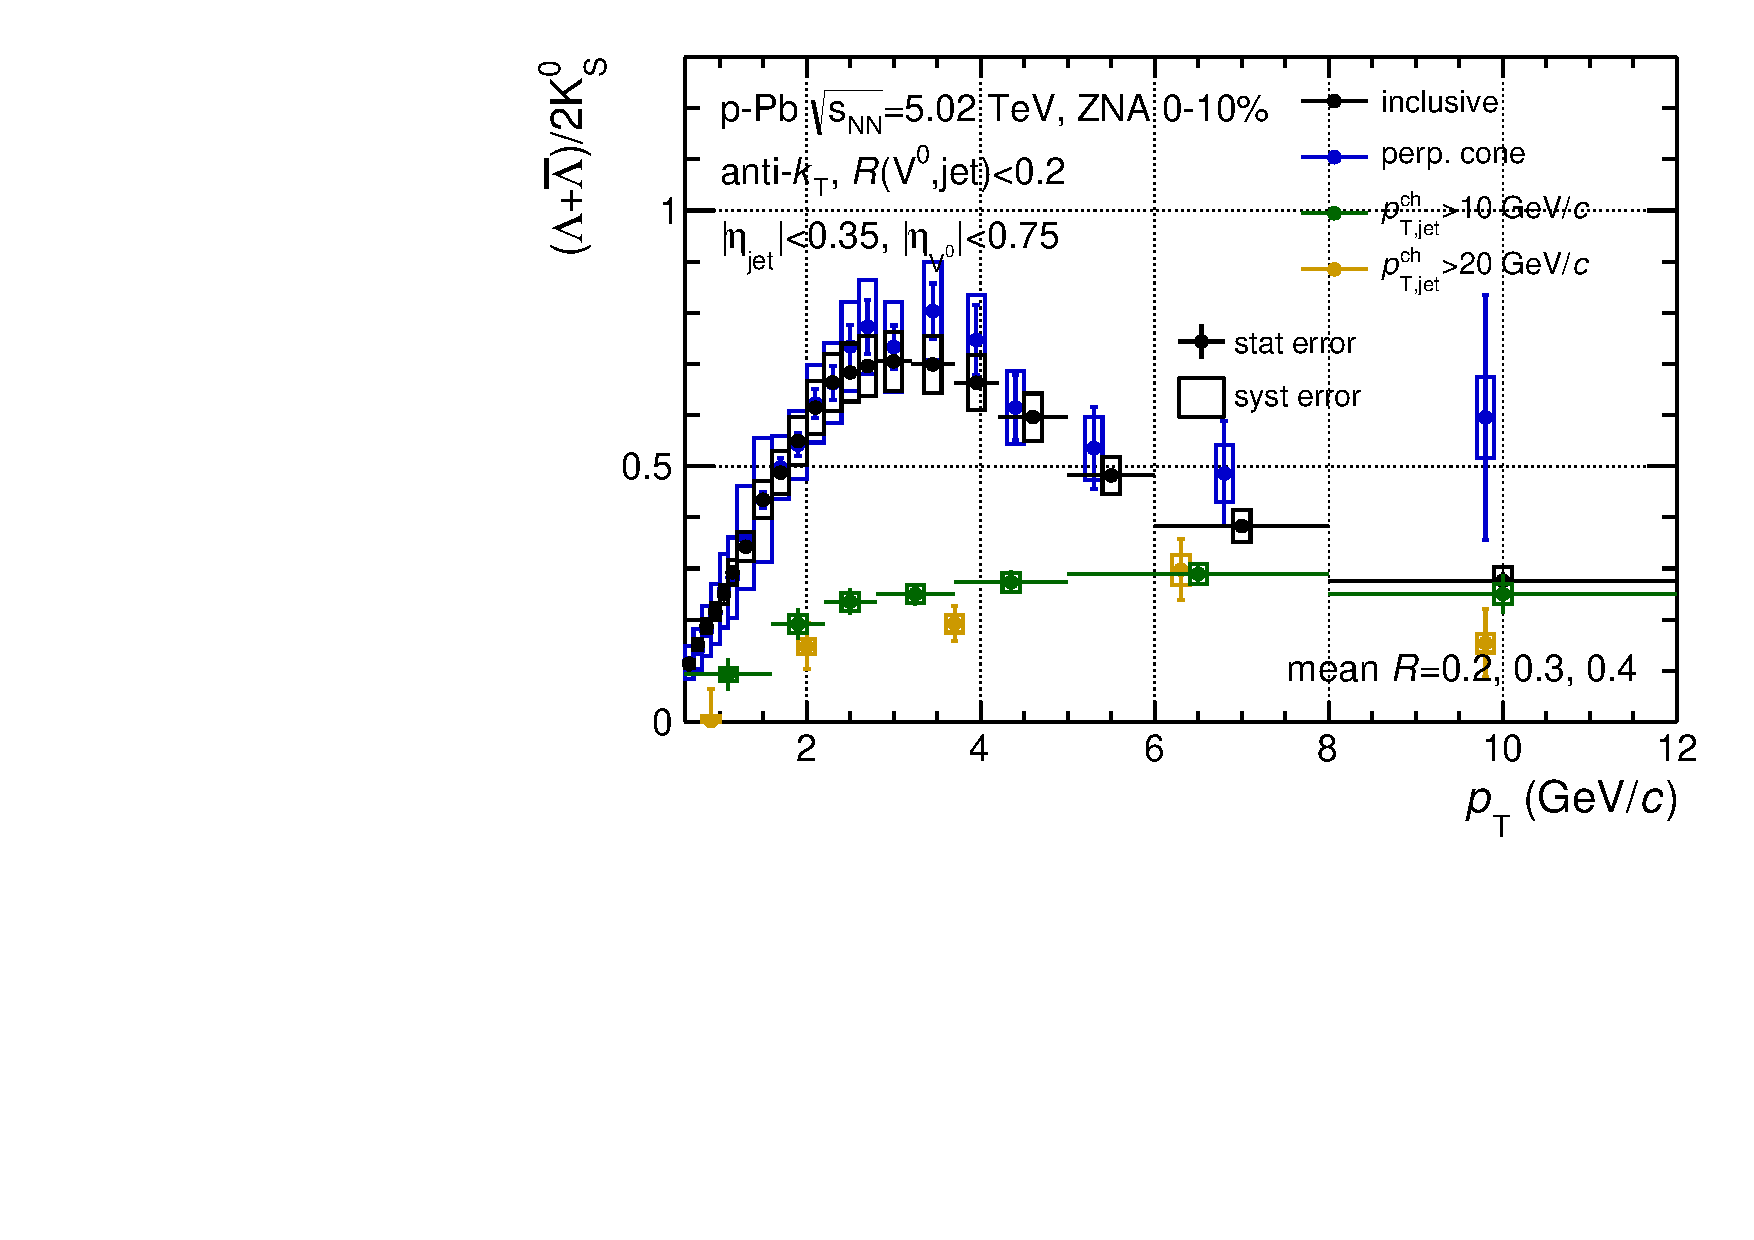
\includegraphics[width=.32\textwidth]{cL2K_Pt_PtJE_JC02_ZNA_000_010}
\caption{$\Lambda$-to-$\Kshort$ ratio as a function of $\pT$
  averaged over jets with
  $R=0.2,~0.3$ and $0.4$ in $p_{\rm T,jet}>10$ and $>20~\GeVc$,
  respectively.
  $\Vzero$--jet matching radius $R(\Vzero,{\rm jet})<0.2$.
  Results are shown in three ZNA event activity classes and
  compared with the inclusive and the underlying $\Vzeros$.}
\label{fig:s01L2KJC02ZNAPtjXX}
\end{figure}

\begin{figure}[htbp]
\centering
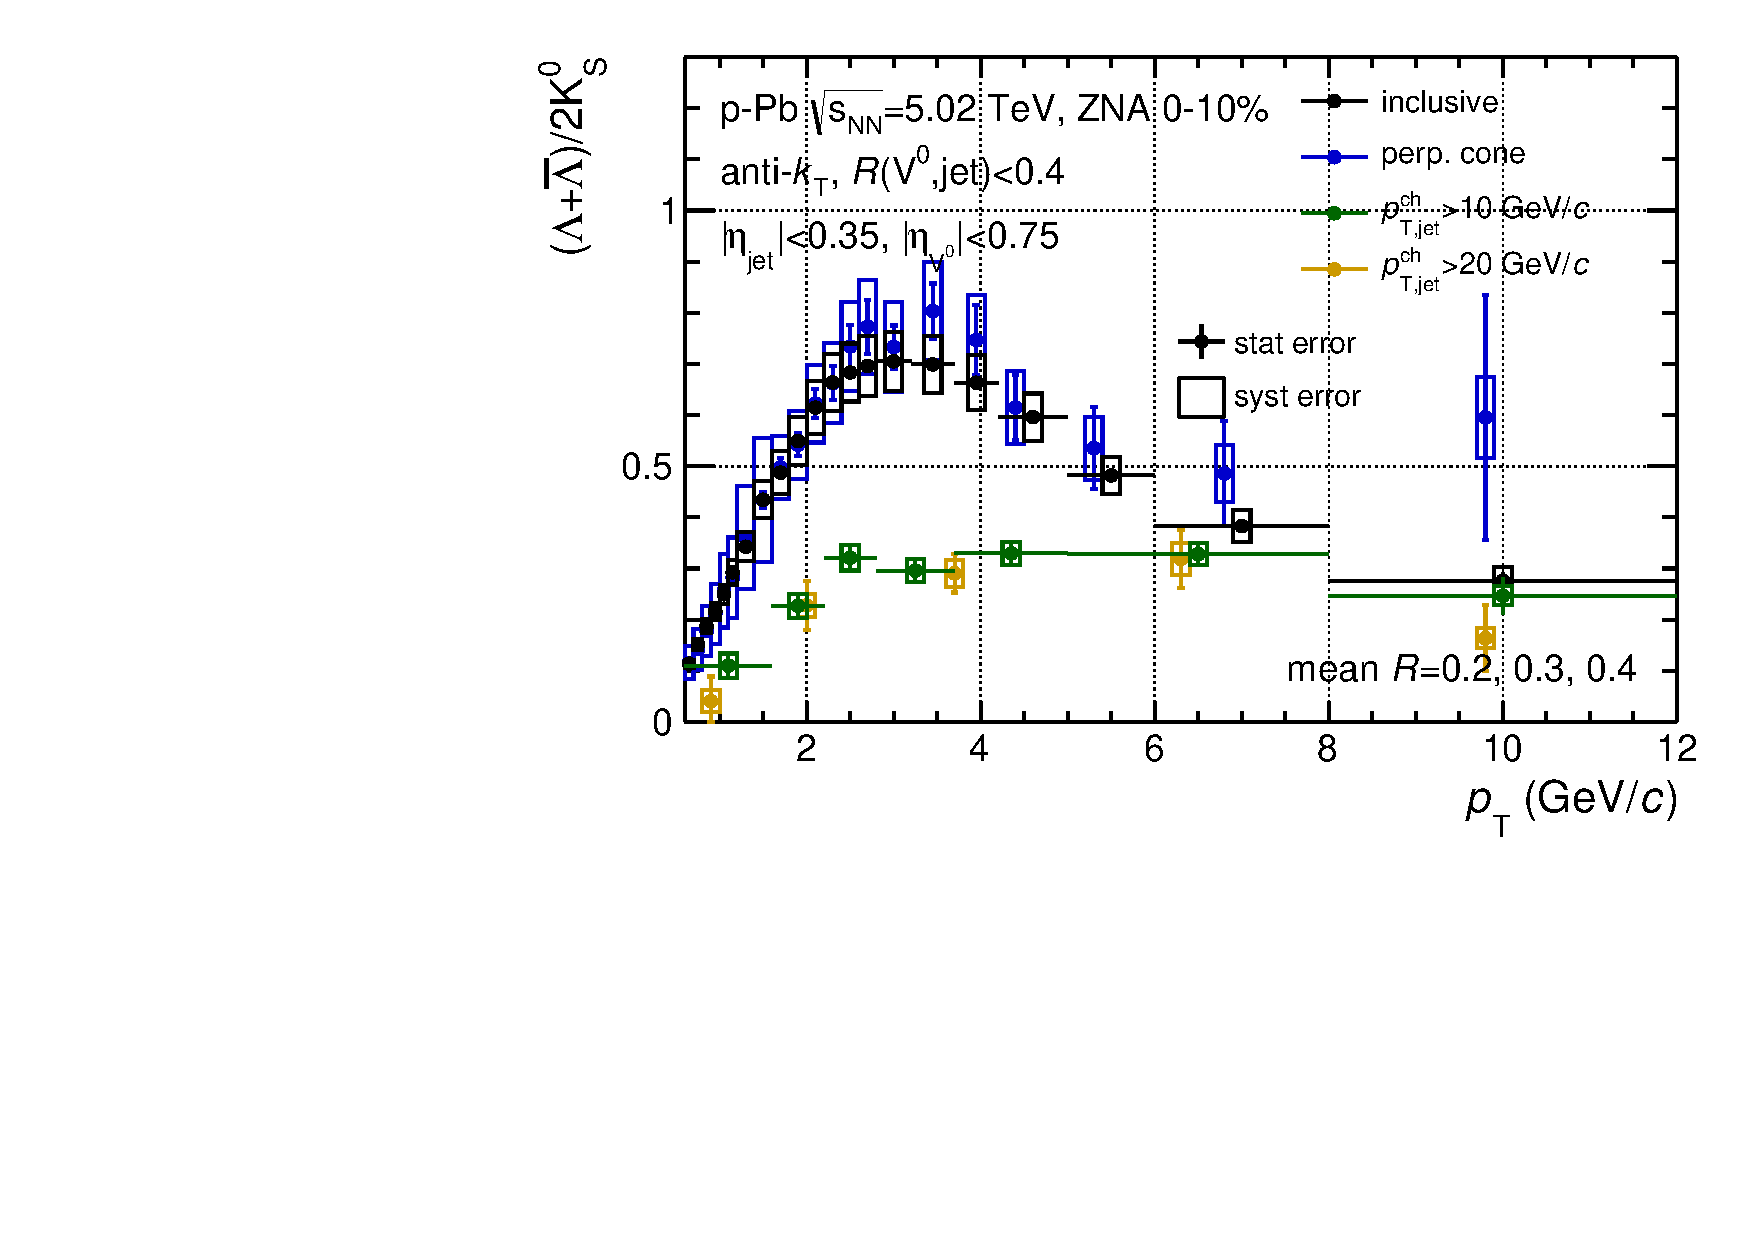
\includegraphics[width=.32\textwidth]{cL2K_Pt_PtJE_JC04_ZNA_000_010}
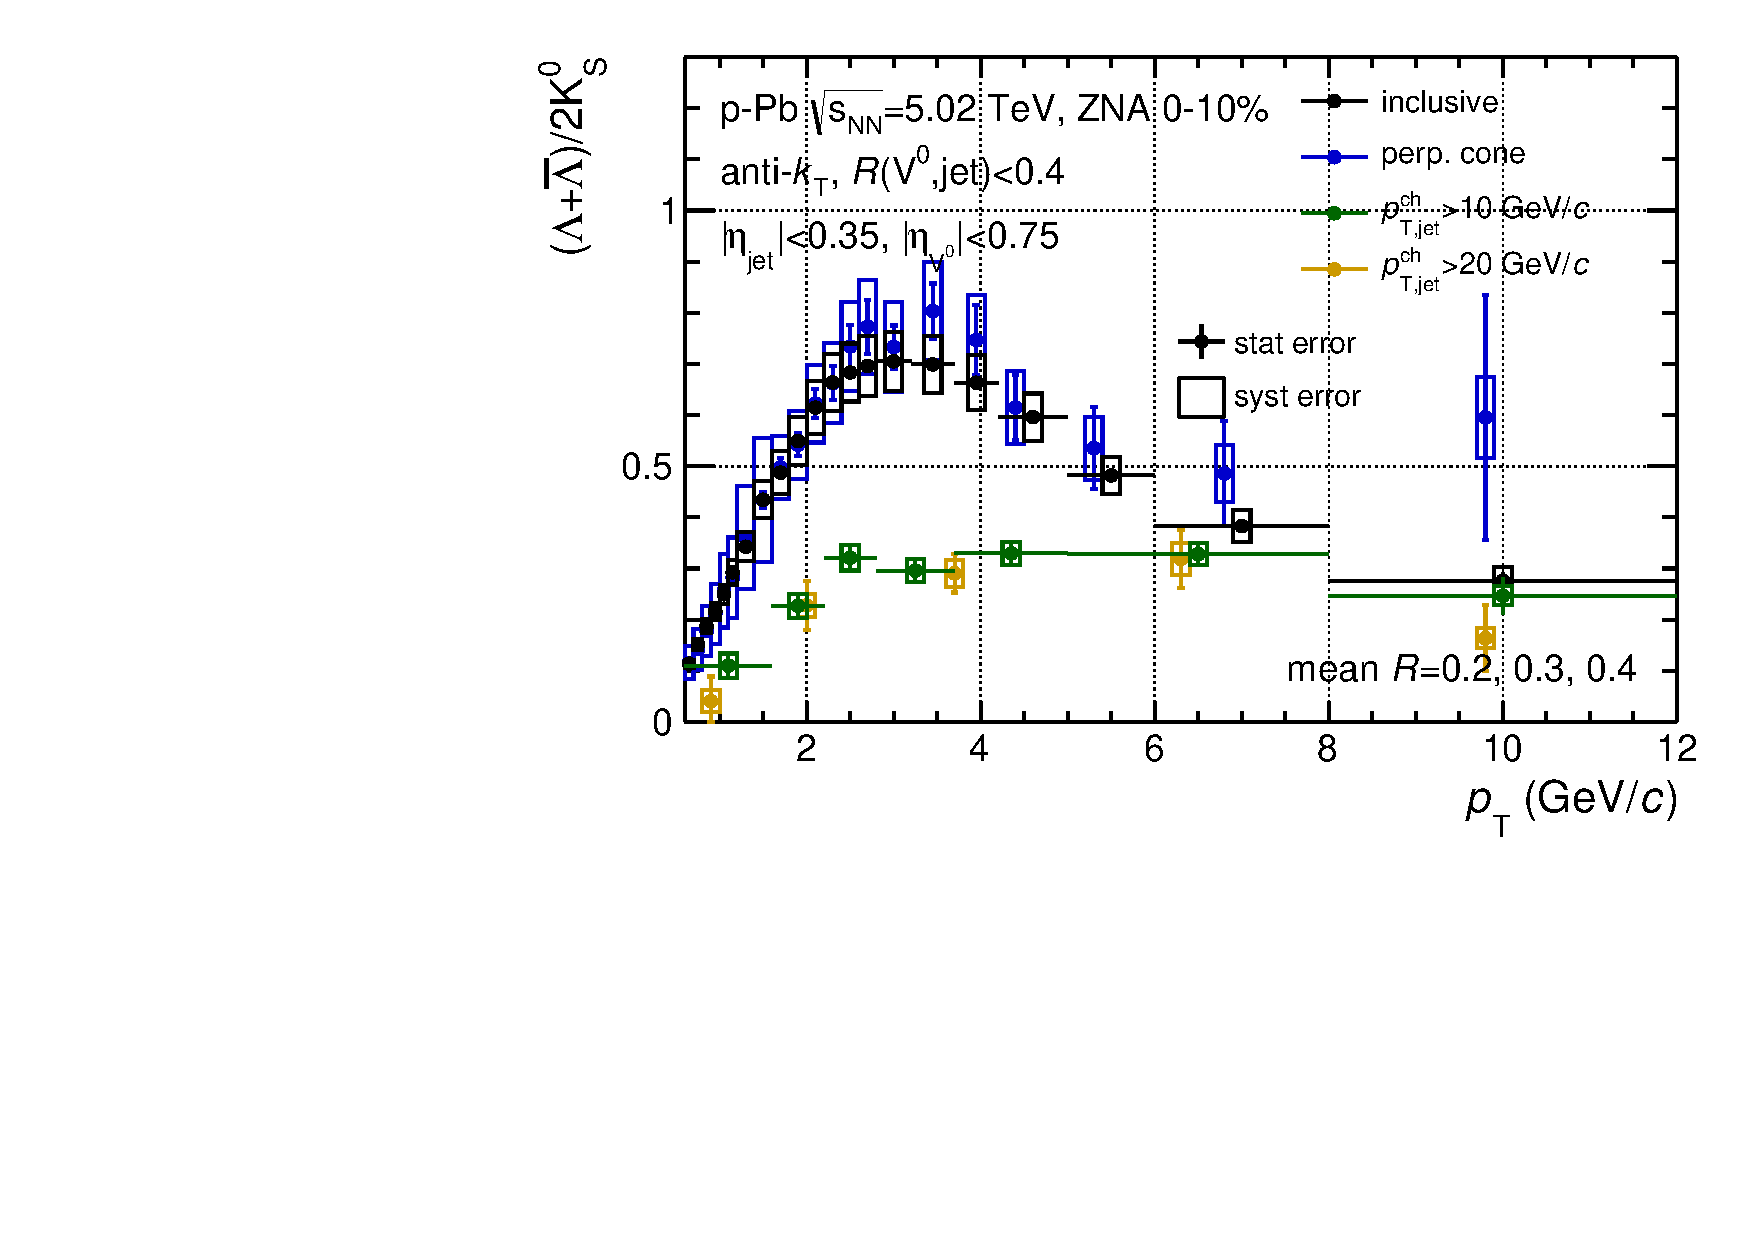
\includegraphics[width=.32\textwidth]{cL2K_Pt_PtJE_JC04_ZNA_000_010}
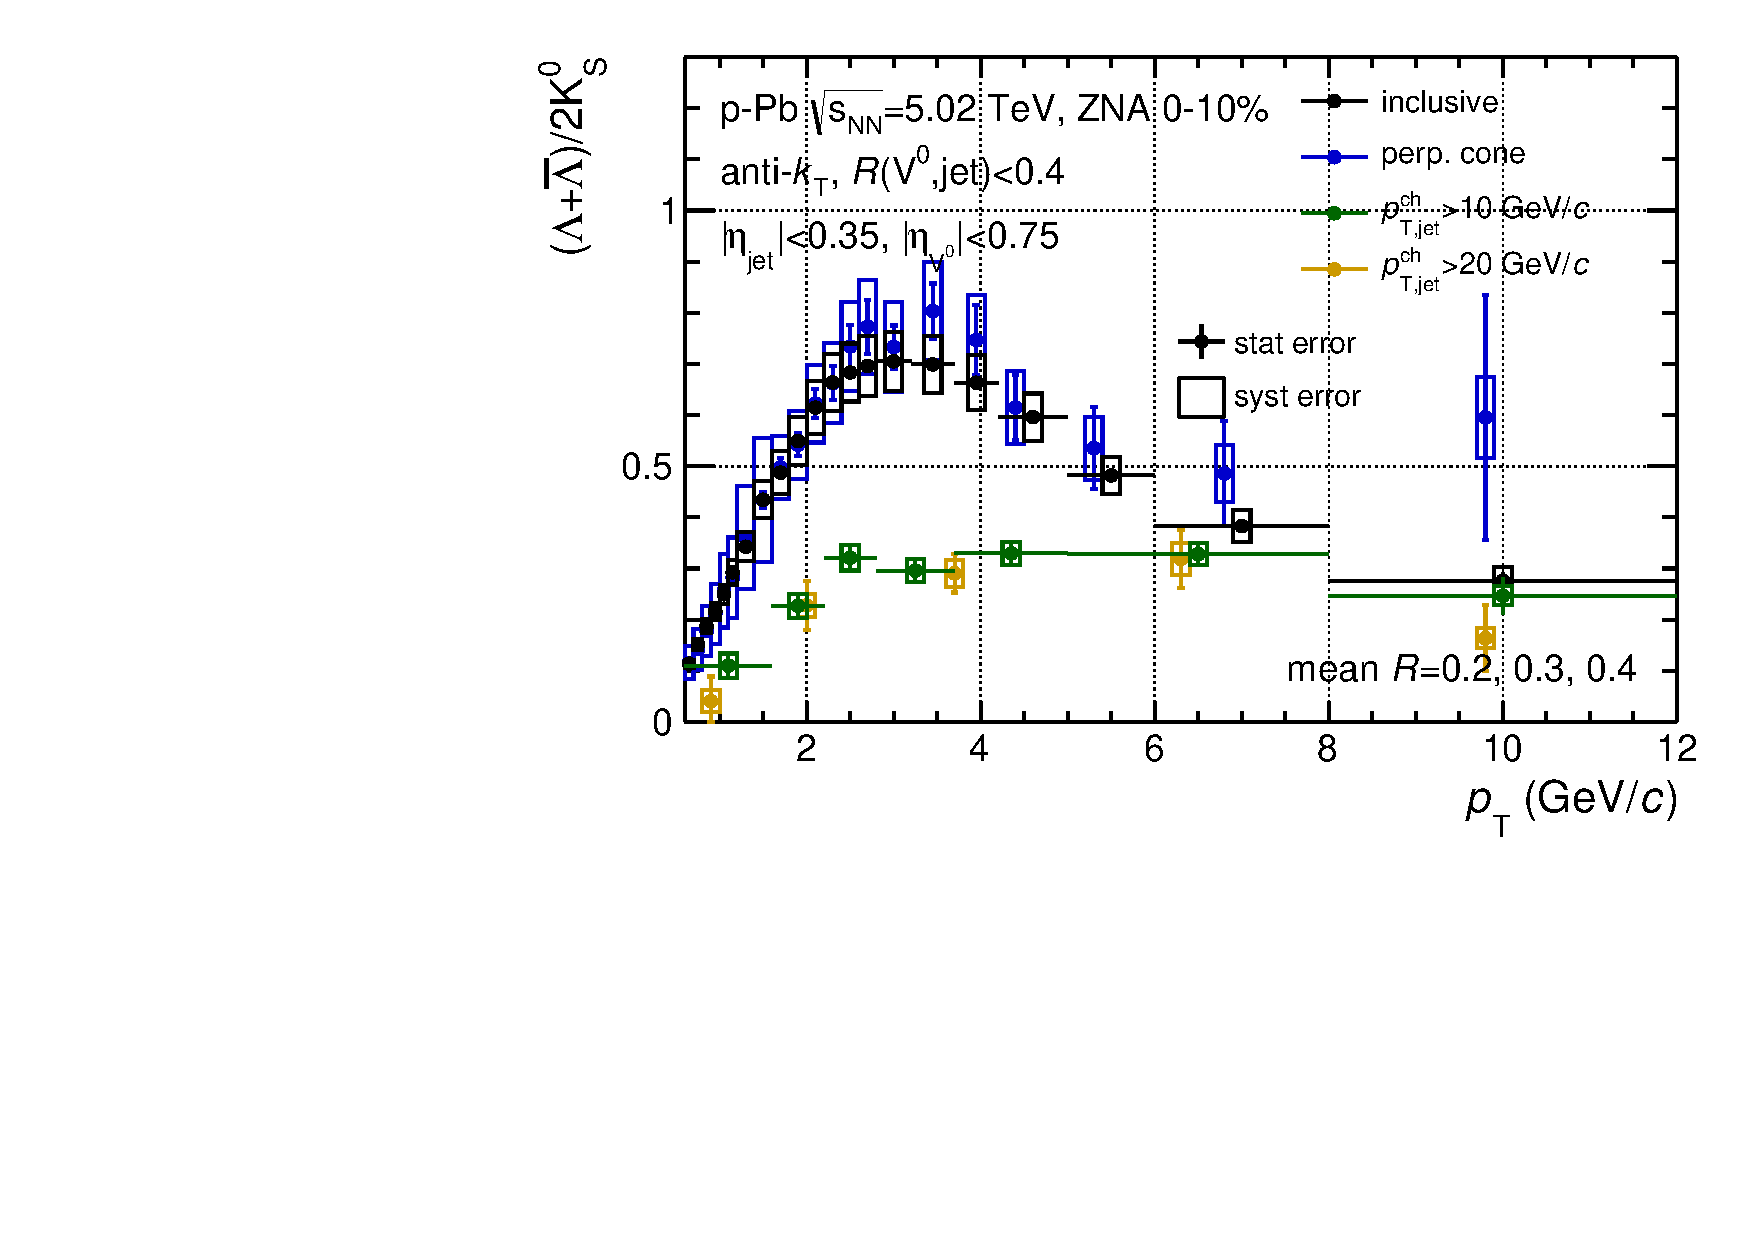
\includegraphics[width=.32\textwidth]{cL2K_Pt_PtJE_JC04_ZNA_000_010}
\caption{$\Lambda$-to-$\Kshort$ ratio as a function of $\pT$
  averaged over jets with
  $R=0.2,~0.3$ and $0.4$ in $p_{\rm T,jet}>10$ and $>20~\GeVc$,
  respectively.
  $\Vzero$--jet matching radius $R(\Vzero,{\rm jet})<0.4$.
  Results are shown in three ZNA event activity classes and
  compared with the inclusive and the underlying $\Vzeros$.}
\label{fig:s01L2KJC04ZNAPtjXX}
\end{figure}
%%%%%%%%%%%%%%%%%%%%%%%%%%%%%%%%%%%%%%%%%%%%%%%%%%%%%%%%%%%%%%%%%%%%%%%%%%%%%%%

\newpage
\section{$\Lambda$-to-$\Kshort$ ratio as a function of matching radius}

\subsection{$\Vzero$ density as a function of matching radius}

\begin{figure}[htbp]
\centering
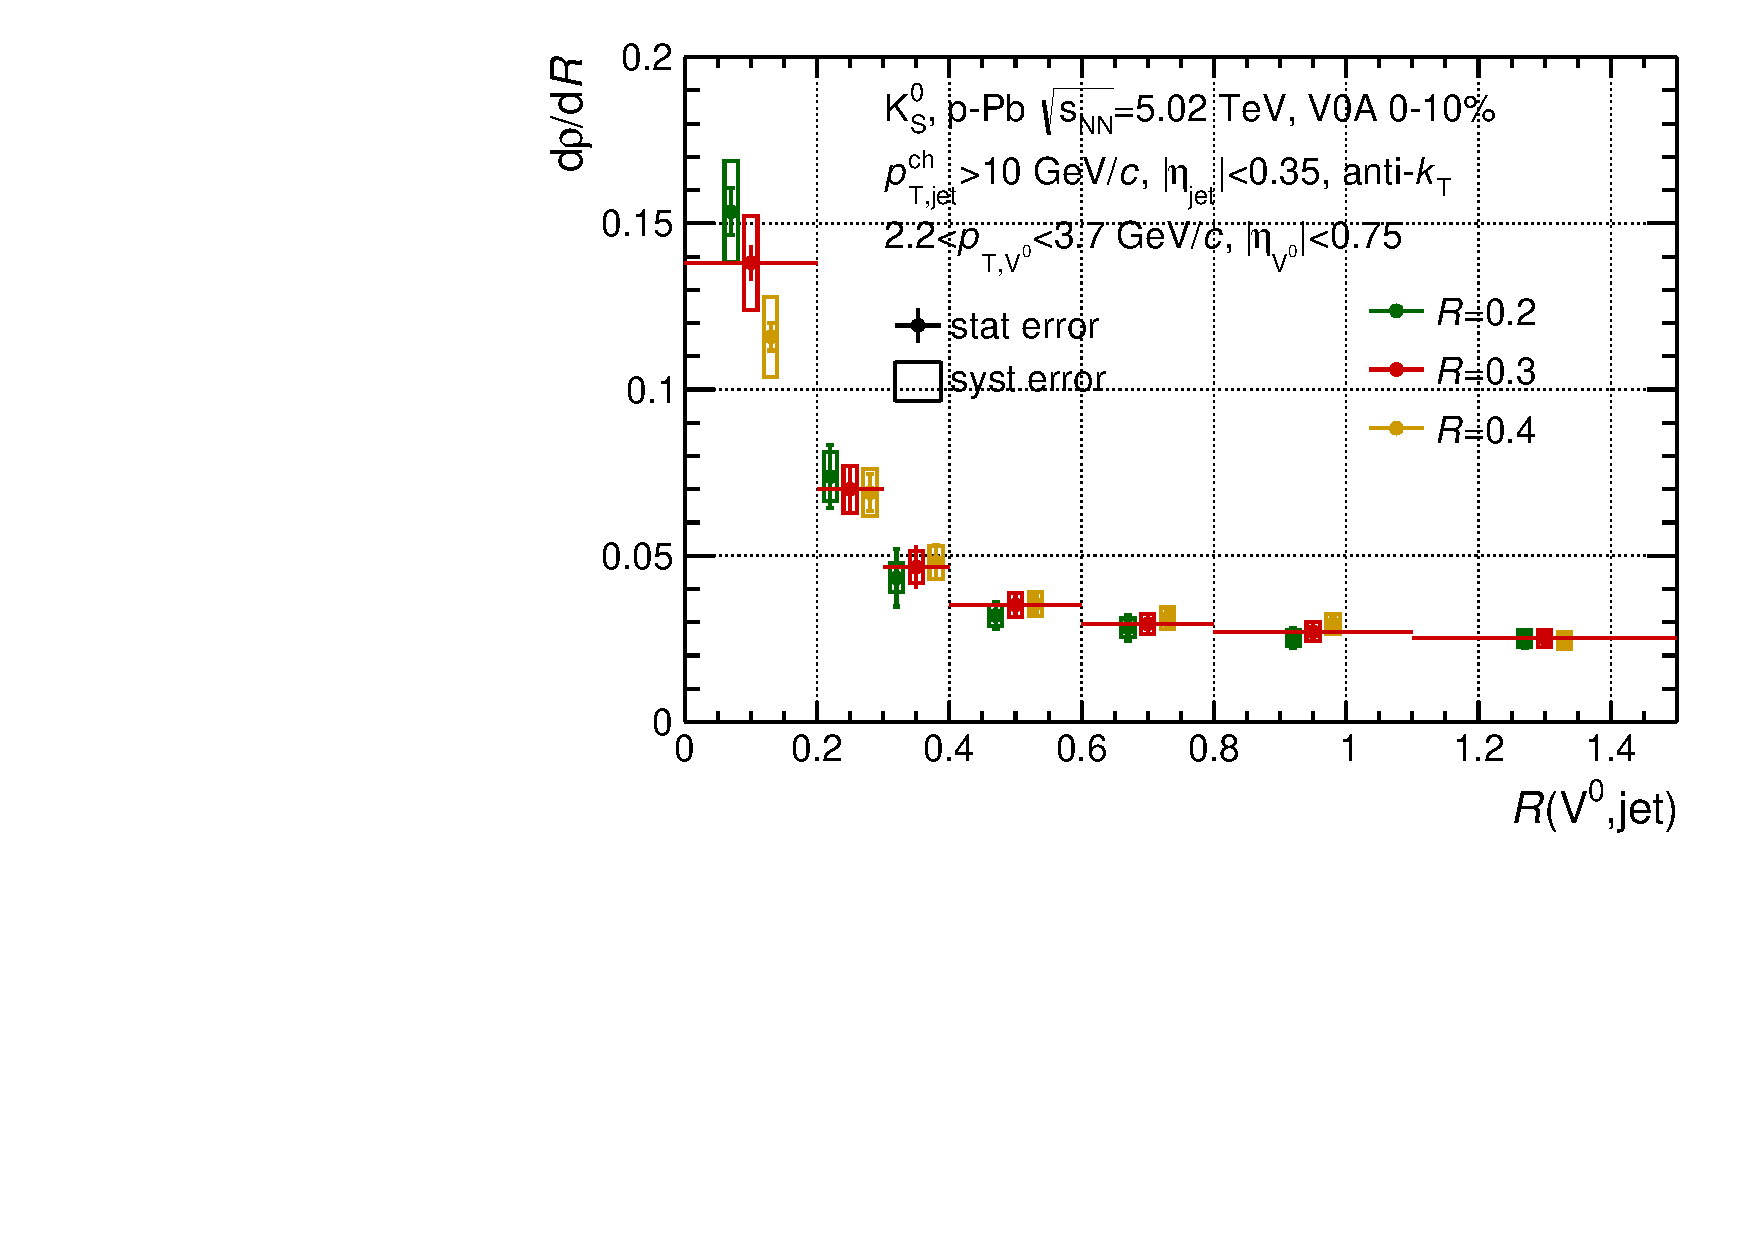
\includegraphics[width=.32\textwidth]{cKshort_VJ_Comp_V0A_000_010_PtJ10_PtV0_2d2_3d7}
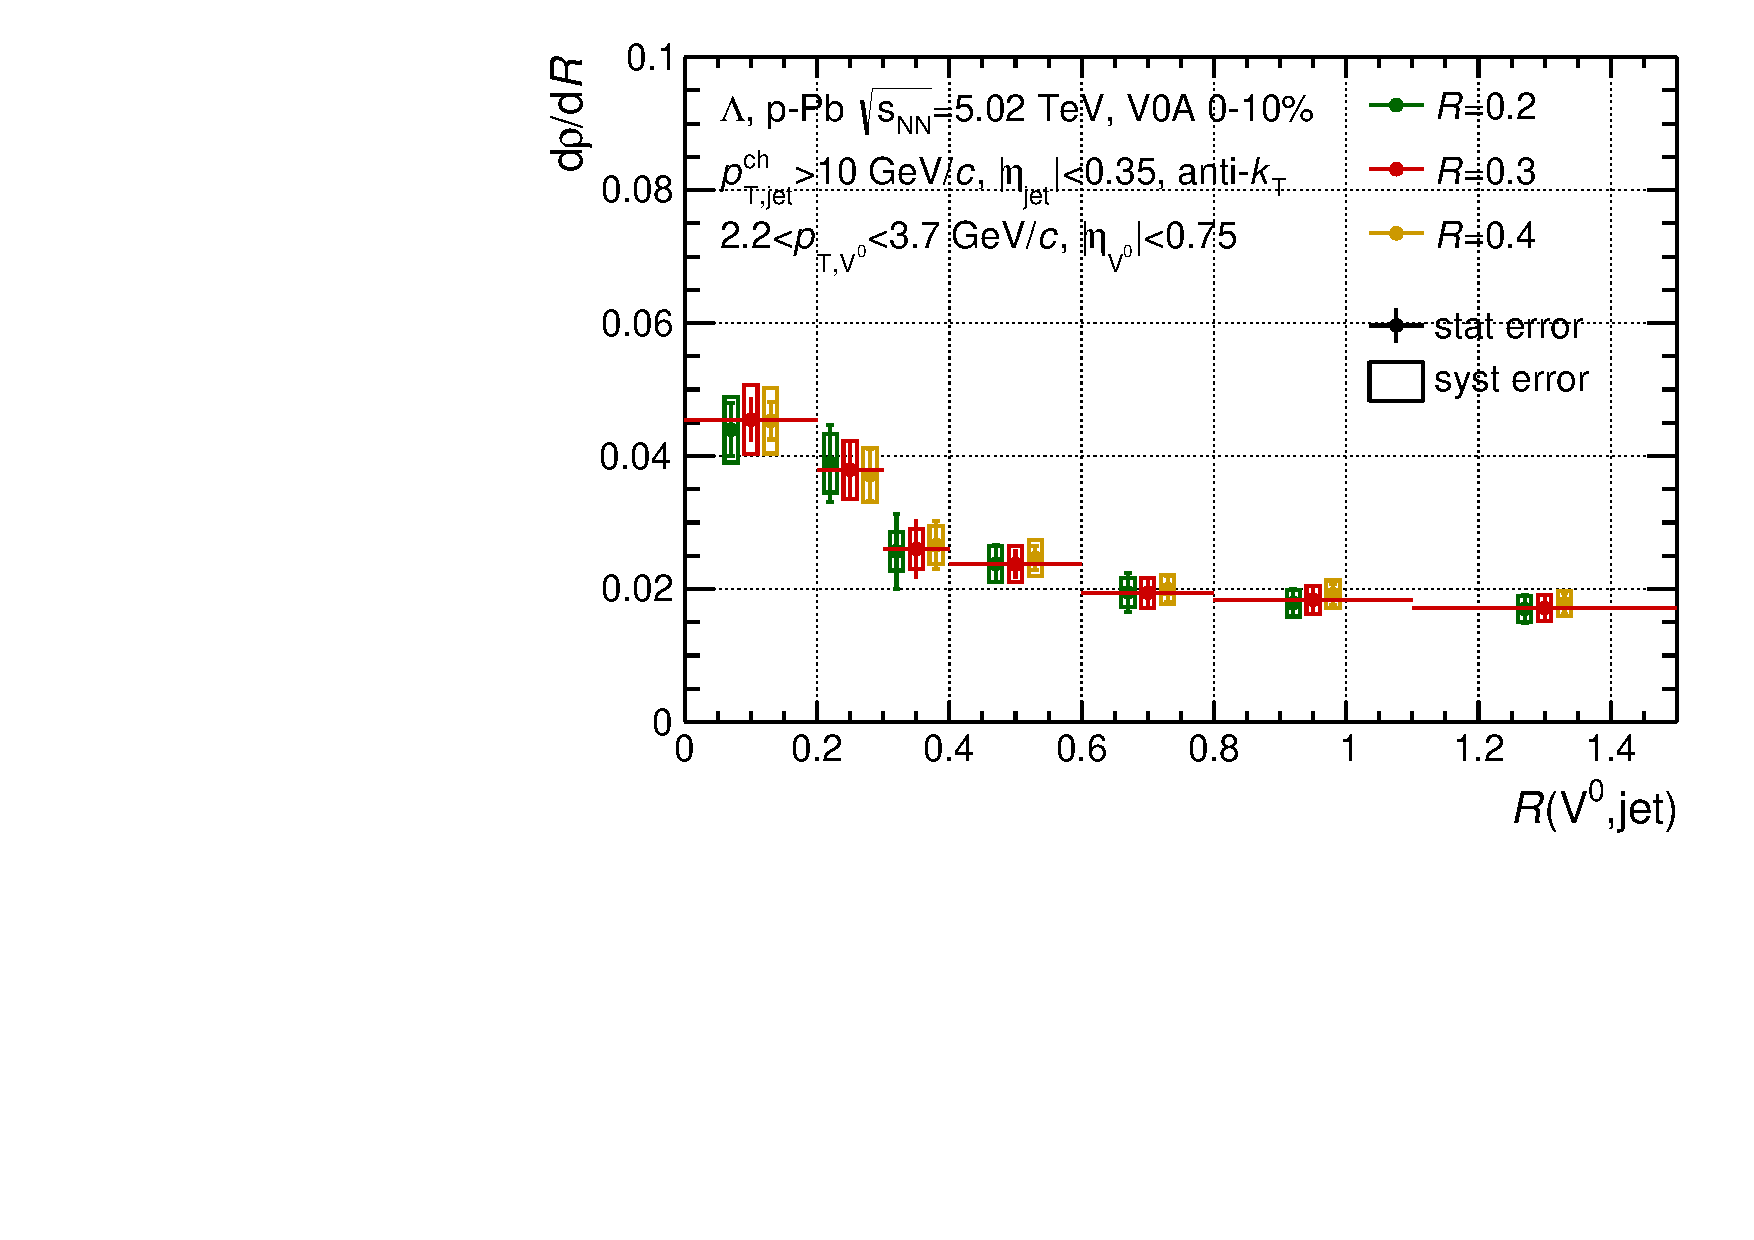
\includegraphics[width=.32\textwidth]{cLambda_VJ_Comp_V0A_000_010_PtJ10_PtV0_2d2_3d7}
\includegraphics[width=.32\textwidth]{cAntiLa_VJ_Comp_V0A_000_010_PtJ10_PtV0_2d2_3d7}
\caption{$\Vzero$ density spectra as a function of matching radius $R(\Vzero,{\rm jet})$ in jets
  with resolution parameters $R=0.2,~0.3$ and $0.4$ and in $p_{\rm T,jet}>10~\GeVc$.
  $\Vzeros$ are obtained in $2.2<\pT<3.7~\GeVc$.
  Results are shown in $0-10\%$ V0A event activity class.
  The underlying $\Vzeros$ are not subtracted.}
\label{fig:s02SpcVJV0APtj10}
\end{figure}
%%%%%%%%%%%%%%%%%%%%%%%%%%%%%%%%%%%%%%%%%%%%%%%%%%%%%%%%%%%%%%%%%%%%%%%%%%%%%%%

\newpage
\subsection{$\Lambda$-to-$\Kshort$ ratio average over jets resolution parameters}

\begin{figure}[htbp]
\centering
\includegraphics[width=.32\textwidth]{cRatioV_VJ_Mean_V0A_000_010_PtJ10}
\includegraphics[width=.32\textwidth]{cRatioV_VJ_Mean_V0A_010_040_PtJ10}
\includegraphics[width=.32\textwidth]{cRatioV_VJ_Mean_V0A_040_100_PtJ10}
\caption{$\Lambda$-to-$\Kshort$ ratio as a function of matching radius $R(\Vzero,{\rm jet})$ in jets
 averaged over resolution parameters $R=0.2,~0.3$ and $0.4$ and in $p_{\rm T,jet}>10~\GeVc$.
 Results are shown in three $\Vzero$ $\pT$ regions and
 three V0A event activity classes.
 The underlying $\Vzeros$ are not subtracted.}
\label{fig:s02L2KVJV0APtj10}
\end{figure}

\begin{figure}[htbp]
\centering
\includegraphics[width=.32\textwidth]{cRatioV_VJ_PtJE_V0A_000_010_PtV0_2d2_3d7}
\includegraphics[width=.32\textwidth]{cRatioV_VJ_PtJE_V0A_010_040_PtV0_2d2_3d7}
\includegraphics[width=.32\textwidth]{cRatioV_VJ_PtJE_V0A_040_100_PtV0_2d2_3d7}
\caption{$\Lambda$-to-$\Kshort$ ratio as a function of matching radius $R(\Vzero,{\rm jet})$ in jets
 averaged over resolution parameters $R=0.2,~0.3$ and $0.4$ and in $p_{\rm T,jet}>10$
 and $20~\GeVc$, respectively.
 Results are shown in $2.2<\pT<3.7~\GeVc$ and
 three V0A event activity classes.
 The underlying $\Vzeros$ are not subtracted.}
\label{fig:s02L2KVJV0APtjXX}
\end{figure}
%%%%%%%%%%%%%%%%%%%%%%%%%%%%%%%%%%%%%%%%%%%%%%%%%%%%%%%%%%%%%%%%%%%%%%%%%%%%%%%

\newpage
\section{Mean $\pT$ of $\Vzeros$}

\subsection{$\Vzero$ mean $\pT$ as a function of event multiplicity}

\begin{figure}[htbp]
\centering
\includegraphics[width=.48\textwidth]{cMeanPt_KaHD}
\includegraphics[width=.48\textwidth]{cMeanPt_LaHD}
\caption{Mean $\pT$ of $\Vzeros$ in jets averaged over resolution parameter $R=0.2,~0.3$
and $0.4$ in varius matching radii and jet $\pT$ regions.}
\label{fig:s02MeanPtHD}
\end{figure}

\begin{figure}[htbp]
\centering
\includegraphics[width=.48\textwidth]{cMeanPt_KaJC}
\includegraphics[width=.48\textwidth]{cMeanPt_LaJC}
\caption{Mean $\pT$ of $\Vzeros$ in jets averaged over resolution parameter $R=0.2,~0.3$
and $0.4$ in varius matching radii and jet $\pT$ regions.
The underlying $\Vzeros$ are not subtracted.}
\label{fig:s03MeanPtJC}
\end{figure}

\begin{figure}[htbp]
\centering
\includegraphics[width=.48\textwidth]{cMeanPt_Comp_JC02_PtJ10_HD}
\includegraphics[width=.48\textwidth]{cMeanPt_Comp_JC02_PtJ10_JC}
\caption{Mean $\pT$ of $\Vzeros$ in jets averaged over resolution parameter $R=0.2,~0.3$
and $0.4$ with $\Vzero$--jet matching radius $R(\Vzero,{\rm jet})<0.2$ and
in $p_{\rm T,jet}>10~\GeVc$.
The results with and without
the underlying $\Vzero$ subtraction are shown in high and left, respectively.}
\label{fig:s03MeanComp}
\end{figure}
%%%%%%%%%%%%%%%%%%%%%%%%%%%%%%%%%%%%%%%%%%%%%%%%%%%%%%%%%%%%%%%%%%%%%%%%%%%%%%%

\newpage
\subsection{$\Vzero$ mean $\pT$ as a function of matching radius}

\begin{figure}[htbp]
\centering
\includegraphics[width=.48\textwidth]{cMeanPt_KaVJ_PtJ10}
\includegraphics[width=.48\textwidth]{cMeanPt_KaVJ_PtJ20}
\caption{Mean $\pT$ of $\Kshort$ as a function of matched radius
in jets averaged over resolution parameter $R=0.2,~0.3$
and $0.4$ in $p_{\rm T,jet}>10$ and $20~\GeVc$.
The underlying $\Vzeros$ are not subtracted.}
\label{fig:s03MeanKaVJ}
\end{figure}

\begin{figure}[htbp]
\centering
\includegraphics[width=.48\textwidth]{cMeanPt_LaVJ_PtJ10}
\includegraphics[width=.48\textwidth]{cMeanPt_LaVJ_PtJ20}
\caption{Mean $\pT$ of $\Lambda+\AntiLa$ as a function of matched radius
in jets averaged over resolution parameter $R=0.2,~0.3$
and $0.4$ in $p_{\rm T,jet}>10$ and $20~\GeVc$.
The underlying $\Vzeros$ are not subtracted.}
\label{fig:s03MeanLaVJ}
\end{figure}

\begin{figure}[htbp]
\centering
\includegraphics[width=.32\textwidth]{cMeanPt_PtVJ_V0A_000_010_Kshort}
\includegraphics[width=.32\textwidth]{cMeanPt_PtVJ_V0A_010_040_Kshort}
\includegraphics[width=.32\textwidth]{cMeanPt_PtVJ_V0A_040_100_Kshort}
\caption{Mean $\pT$ and $\Kshort$ as a function of matched radius
in jets averaged over resolution parameter $R=0.2,~0.3$
and $0.4$ in $p_{\rm T,jet}>10~\GeVc$ and $20~\GeVc$.
Results are shown in three V0A event activity classes.
The underlying $\Vzeros$ are not subtracted.}
\label{fig:s03MeanActLaVJ}
\end{figure}

\begin{figure}[htbp]
\centering
\includegraphics[width=.32\textwidth]{cMeanPt_PtVJ_V0A_000_010_Lambda}
\includegraphics[width=.32\textwidth]{cMeanPt_PtVJ_V0A_010_040_Lambda}
\includegraphics[width=.32\textwidth]{cMeanPt_PtVJ_V0A_040_100_Lambda}
\caption{Mean $\pT$ of $\Lambda+\AntiLa$ as a function of matched radius
in jets averaged over resolution parameter $R=0.2,~0.3$
and $0.4$ in $p_{\rm T,jet}>10$ and $20~\GeVc$.
Results are shown in three V0A event activity classes.
The underlying $\Vzeros$ are not subtracted.}
\label{fig:s03MeanActLaVJ}
\end{figure}

\begin{figure}[htbp]
\centering
\includegraphics[width=.48\textwidth]{cMeanPt_V0VJ_V0A_000_010_PtJ10}
\includegraphics[width=.48\textwidth]{cMeanPt_V0VJ_V0A_000_010_PtJ20}
\caption{Mean $\pT$ of $\Vzeros$ as a function of matched radius
in jets averaged over resolution parameter $R=0.2,~0.3$
and $0.4$ in $p_{\rm T,jet}>10~\GeVc$.
The underlying $\Vzeros$ are not subtracted.}
\label{fig:s03MeanV0VJ}
\end{figure}

\begin{figure}[htbp]
\centering
\includegraphics[width=.32\textwidth]{cMeanPt_V0VJ_V0A_000_010_PtJ10}
\includegraphics[width=.32\textwidth]{cMeanPt_V0VJ_V0A_010_040_PtJ10}
\includegraphics[width=.32\textwidth]{cMeanPt_V0VJ_V0A_040_100_PtJ10}
\caption{Mean $\pT$ of $\Vzeros$ as a function of matched radius
in jets averaged over resolution parameter $R=0.2,~0.3$
and $0.4$ in $p_{\rm T,jet}>10~\GeVc$.
Results are shown in three V0A event activity classes.
The underlying $\Vzeros$ are not subtracted.}
\label{fig:s03MeanActV0VJ}
\end{figure}

\end{document}
